\appendix
\section{Doubling supply does not double successful matches}
%\bbcomment{edited title}
\label{sec: example_introduction}

This section complements 
\Cref{sec: introduction} and illustrates that there is an $2$-undersupplied instance in which doubling the available supply does not double the number successful matches.
Let $\prob = 1/n$ for a large $n \in \mathbb{N}$. Consider the instance $\inst$ constructed as follows (see \Cref{fig:2-undersupplied_instance_1}): there is one supply node $u_1$ connected to $2/\prob$ demand nodes $v_1, \ldots, v_{2/\prob}$, where each edge exists independently with probability $\prob$. Since there are $2/\prob$ demand nodes $\offI(\inst) = 1$ and $\offI(\inst, 2) = 2 \cdot \offI(\inst)$, i.e., $\inst$ is $2$-undersupplied. Clearly, the optimal algorithm achieves $\text{ALG}(\inst) = 1 - (1-\prob)^{2/\prob} \approx 1 - e^{-2}$.

Now, consider the instance $\inst'$ (see \Cref{fig:2-undersupplied_instance_2}) that is achieved by duplicating the available supply; we consider a second supply node $u_2$ connected to every demand node. By concavity of $1-(1-\prob)^x$, the optimal algorithm in $\inst'$ allocates $1/\prob$ demand nodes to each supply node, which results in $$\text{ALG}(\inst') = 2 \cdot \left(1 - (1-\prob)^{1/\prob}\right) \approx 2 \cdot (1 - e^{-1}) = 2 \cdot (1 - e^{-1}) \cdot \offI(\inst).$$

\begin{figure}[h]
    \centering
    \tikzset{every picture/.style={line width=0.75pt}} 
    % First minipage
    \begin{minipage}[b]{0.45\textwidth}
        \centering
        
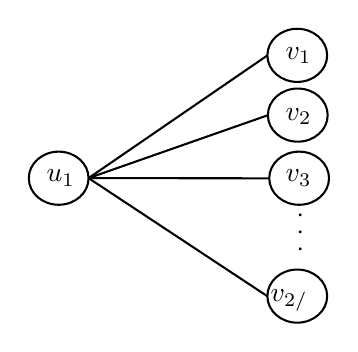
\begin{tikzpicture}[x=0.75pt,y=0.75pt,yscale=-0.8,xscale=.9]
%uncomment if require: \path (0,310); %set diagram left start at 0, and has height of 310
%set default line width to 0.75pt        
%Shape: Circle [id:dp705325080636104] 
\draw   (237.14,68.73) .. controls (237.17,77.56) and (230.04,84.76) .. (221.2,84.79) .. controls (212.37,84.83) and (205.17,77.7) .. (205.14,68.86) .. controls (205.1,60.02) and (212.23,52.83) .. (221.07,52.79) .. controls (229.91,52.76) and (237.1,59.89) .. (237.14,68.73) -- cycle ;
%Shape: Circle [id:dp9045264439682683] 
\draw   (236.86,32.73) .. controls (236.9,41.56) and (229.76,48.76) .. (220.93,48.79) .. controls (212.09,48.83) and (204.9,41.7) .. (204.86,32.86) .. controls (204.82,24.03) and (211.96,16.83) .. (220.79,16.8) .. controls (229.63,16.76) and (236.82,23.89) .. (236.86,32.73) -- cycle ;
%Shape: Circle [id:dp7330157492007956] 
\draw   (109.14,106.73) .. controls (109.17,115.56) and (102.04,122.76) .. (93.2,122.79) .. controls (84.37,122.83) and (77.17,115.7) .. (77.14,106.86) .. controls (77.1,98.02) and (84.23,90.83) .. (93.07,90.79) .. controls (101.91,90.76) and (109.1,97.89) .. (109.14,106.73) -- cycle ;
%Straight Lines [id:da6695348841913797] 
\draw    (109.14,106.73) -- (204.86,32.86) ;
%Straight Lines [id:da13011748270531487] 
\draw    (109.14,106.73) -- (205.14,68.86) ;
%Shape: Circle [id:dp2858628406519379] 
\draw   (237.86,106.73) .. controls (237.9,115.56) and (230.76,122.76) .. (221.93,122.79) .. controls (213.09,122.83) and (205.9,115.7) .. (205.86,106.86) .. controls (205.82,98.03) and (212.96,90.83) .. (221.79,90.8) .. controls (230.63,90.76) and (237.82,97.89) .. (237.86,106.73) -- cycle ;
%Shape: Circle [id:dp3861940620968769] 
\draw   (236.86,177.73) .. controls (236.9,186.56) and (229.76,193.76) .. (220.93,193.79) .. controls (212.09,193.83) and (204.9,186.7) .. (204.86,177.86) .. controls (204.82,169.03) and (211.96,161.83) .. (220.79,161.8) .. controls (229.63,161.76) and (236.82,168.89) .. (236.86,177.73) -- cycle ;
%Straight Lines [id:da5206970800834672] 
\draw    (109.14,106.73) -- (205.86,106.86) ;
%Straight Lines [id:da9103551306429898] 
\draw    (109.14,106.73) -- (204.86,177.86) ;

% Text Node
\draw (213,63) node [anchor=north west][inner sep=0.75pt]   [align=left] {{$v_2$}};
% Text Node
\draw (213,26) node [anchor=north west][inner sep=0.75pt]   [align=left] {{$v_1$}};
% Text Node
\draw (85,100) node [anchor=north west][inner sep=0.75pt]   [align=left] {{$u_1$}};
% Text Node
\draw (225, 125) node [anchor=north west][inner sep=0.75pt]  [rotate=-90.1]  {$.\ .\ .$};
% Text Node
\draw (213,100) node [anchor=north west][inner sep=0.75pt]   [align=left] {{$v_3$}};
% Text Node
\draw (205,172) node [anchor=north west][inner sep=0.75pt]   [align=left] {{$v_{2/\prob}$}};


\end{tikzpicture}
        \caption{The described instance $\inst$. Each edge has a probability of success $\prob = 1/n$.}
        \label{fig:2-undersupplied_instance_1}
    \end{minipage}
    \hfill
    % Second minipage
    \begin{minipage}[b]{0.45\textwidth}
        \centering
        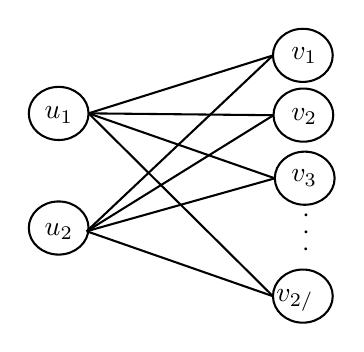
\begin{tikzpicture}[x=0.75pt,y=0.75pt,yscale=-.8,xscale=.9]
%uncomment if require: \path (0,310); %set diagram left start at 0, and has height of 310

%Shape: Circle [id:dp6090523810369015] 
\draw   (237.14,68.73) .. controls (237.17,77.56) and (230.04,84.76) .. (221.2,84.79) .. controls (212.37,84.83) and (205.17,77.7) .. (205.14,68.86) .. controls (205.1,60.02) and (212.23,52.83) .. (221.07,52.79) .. controls (229.91,52.76) and (237.1,59.89) .. (237.14,68.73) -- cycle ;
%Shape: Circle [id:dp34034203493197035] 
\draw   (236.86,32.73) .. controls (236.9,41.56) and (229.76,48.76) .. (220.93,48.79) .. controls (212.09,48.83) and (204.9,41.7) .. (204.86,32.86) .. controls (204.82,24.03) and (211.96,16.83) .. (220.79,16.8) .. controls (229.63,16.76) and (236.82,23.89) .. (236.86,32.73) -- cycle ;
%Shape: Circle [id:dp5539092128290439] 
\draw   (106.14,67.73) .. controls (106.17,76.56) and (99.04,83.76) .. (90.2,83.79) .. controls (81.37,83.83) and (74.17,76.7) .. (74.14,67.86) .. controls (74.1,59.02) and (81.23,51.83) .. (90.07,51.79) .. controls (98.91,51.76) and (106.1,58.89) .. (106.14,67.73) -- cycle ;
%Straight Lines [id:da14320933738311203] 
\draw    (106.14,67.73) -- (204.86,32.86) ;
%Straight Lines [id:da9972820683180388] 
\draw    (106.14,67.73) -- (205.14,68.86) ;
%Shape: Circle [id:dp47025235161463175] 
\draw   (237.86,106.73) .. controls (237.9,115.56) and (230.76,122.76) .. (221.93,122.79) .. controls (213.09,122.83) and (205.9,115.7) .. (205.86,106.86) .. controls (205.82,98.03) and (212.96,90.83) .. (221.79,90.8) .. controls (230.63,90.76) and (237.82,97.89) .. (237.86,106.73) -- cycle ;
%Shape: Circle [id:dp9312202228677839] 
\draw   (236.86,177.73) .. controls (236.9,186.56) and (229.76,193.76) .. (220.93,193.79) .. controls (212.09,193.83) and (204.9,186.7) .. (204.86,177.86) .. controls (204.82,169.03) and (211.96,161.83) .. (220.79,161.8) .. controls (229.63,161.76) and (236.82,168.89) .. (236.86,177.73) -- cycle ;
%Straight Lines [id:da9853234785703398] 
\draw    (106.14,67.73) -- (205.86,106.86) ;
%Straight Lines [id:da9139950255080356] 
\draw    (106.14,67.73) -- (204.86,177.86) ;
%Shape: Circle [id:dp6399629287861359] 
\draw   (106.14,136.73) .. controls (106.17,145.56) and (99.04,152.76) .. (90.2,152.79) .. controls (81.37,152.83) and (74.17,145.7) .. (74.14,136.86) .. controls (74.1,128.02) and (81.23,120.83) .. (90.07,120.79) .. controls (98.91,120.76) and (106.1,127.89) .. (106.14,136.73) -- cycle ;
%Straight Lines [id:da5837878021836072] 
\draw    (105.14,138.73) -- (204.86,177.86) ;
%Straight Lines [id:da910461407022163] 
\draw    (105.14,138.73) -- (205.86,106.86) ;
%Straight Lines [id:da11065517086468435] 
\draw    (105.14,138.73) -- (205.14,68.86) ;
%Straight Lines [id:da5331802739099747] 
\draw    (105.14,138.73) -- (204.86,32.86) ;

% Text Node
\draw (213,63) node [anchor=north west][inner sep=0.75pt]   [align=left] {{$v_2$}};
% Text Node
\draw (213,26) node [anchor=north west][inner sep=0.75pt]   [align=left] {{$v_1$}};
% Text Node
\draw (81,62) node [anchor=north west][inner sep=0.75pt]   [align=left] {{$u_1$}};
% Text Node
\draw (225, 125) node [anchor=north west][inner sep=0.75pt]  [rotate=-90.1]  {$.\ .\ .$};
% Text Node
\draw (213,100) node [anchor=north west][inner sep=0.75pt]   [align=left] {{$v_3$}};
% Text Node
\draw (205,172) node [anchor=north west][inner sep=0.75pt]   [align=left] {{$v_{2/\prob}$}};
% Text Node
\draw (81,132) node [anchor=north west][inner sep=0.75pt]   [align=left] {{$u_2$}};


\end{tikzpicture}
        \caption{The described instance $\inst'$. Each edge has a probability of success of $\prob = 1/n$.}
        \label{fig:2-undersupplied_instance_2}
    \end{minipage}
\end{figure}



\section{Proof of \Cref{lemma: offline is upper bound} (Section \ref{sec: model})}
\label{proof: offline is upper bound}
    Fix any instance $\inst$ and consider $\alg$ any optimal clairvoyant algorithm and $v_1, \ldots, v_T$ a sequence of demand arrivals.  Let $X_{u,t}$ the random indicator variable that indicates if the $t$-th arrival is matched to $u$ and the match is successful, following the decisions from $\alg$. Similarly, 
   let $Y_{u,t}$ the random indicator variable that indicates if the $t$-th arrival is matched to $u$. Note that, for adversarial arrivals, if $(u,t) \in E$ then $\mathbb E[X_{u,t}] = \prob \cdot \mathbb E[Y_{u,t}]$. Similarly, for stochastic arrivals, if $v_t = v$ then $\mathbb E[X_{u,t}] = \prob_{u,v} \cdot \mathbb E[Y_{u,t}]$.
   % Note that, for stochastic arrivals, $\mathbb E[X_{u,t}] = \prob_{u,v} \cdot \mathbb E[Y_{u,t}]$ where $Y_{u,t}$ is the random indicator variable that indicates if the $t$-th arrival is matched to $u$. For adversarial arrivals the equation holds with $\mathbb E[X_{u,t}] = \prob \cdot \mathbb E[Y_{u,t}]$. Hence, the expected reward of $\alg$ is given by $\mathbb E[\sum_{u,t} X_{u,t}] = \sum_{u,t} \prob_{u,v} \cdot \mathbb E[Y_{u,t}]$. 
   We will prove that $(\mathbb E[Y_{u,t}])_{u \in \supply, t \in [T]}$ can be transformed into a feasible solution to the respective LP, $\offI(\inst, 1)$ with objective value equal to $\mathbb E[\sum_{(u,t) \in \supply \times [T]}  X_{u,t}]$, depending on the arrival model.
   % By padding with zeros if $v_t \not = v$, we extend this solution to $(Y_{u,v})_{(u,v) \in U \times V}$. Independently from the setting, we will prove that $(\mathbb E[Y_{u,v}])_{(u,v) \in U \times V}$ is a feasible solution to the respective LP.

   \begin{enumerate}
       \item \textit{Adversarial arrivals.}  On any given realization $\sum_{t: (u,t) \in E}  X_{u,t} \leq 1$, for all $u \in \supply$ since any supply vertex $u$ can be consumed at most once. By taking expectations, we arrive at $\sum_{t: (u,t) \in E}  \prob \cdot \mathbb E[Y_{u,t}] \leq 1$ and constraint \eqref{adversarial_lp: kappa-constraint} follows. Furthermore, since any arriving demand node $t$ can be matched at most once we have $\sum_{u: (u,t) \in E} Y_{u,t} \leq 1$ for all $t \in [T]$ and hence constraint \eqref{adversarial_lp: demand_constraint} follows by taking expectations. The expected reward of $\alg$ in this arrival model is $\sum_{(u,t) \in \supply \times [T]}  \mathbb E[X_{u,t}] = \mathbb E[\sum_{(u,t) \in E}  X_{u,t}]$ and can be re-written as $\sum_{(u,t) \in E} \prob \cdot \mathbb E[Y_{u,t}]$. Hence, $(\mathbb E[Y_{u,t}])_{(u,t) \in E}$ is a feasible solution to $\offI(\inst)$ with objective $\sum_{(u,t) \in E} \prob \cdot \mathbb E[Y_{u,t}]$.

       \item \textit{Stochastic arrivals.} For all $(u,v) \in \supply \times V$, define $X_{u,v} = \sum_{t \in [T]: v_t = v} X_{u,t}$ the random variable that indicates if a given demand type $v$ consumed a supply node $u$. Similarly, define $Y_{u,v} = \sum_{t \in [T]: v_t = v} Y_{u,t}$. On any given realization we have $\sum_{v \in V}  X_{u,v} \leq 1$, for all $u \in \supply$ since any supply node can be consumed at most once. By taking expectations, we arrive at $\sum_{v \in V}  \prob_{u,v} \cdot \mathbb E[Y_{u,t}] \leq 1$ and constraint \eqref{stochastic_lp: kappa-constraint} follows. Furthermore, any type $v \in V$ can be matched at most $N_v = |\{ v_{t} : v_t = v\}|$ times and hence $\sum_{u \in \supply} Y_{u,v} \leq N_v$ for all $v \in V$. Constraint \eqref{stochastic_lp: demand_constraint} follows by taking expectations and noting that $\mathbb E[N_v] = T p_v$. The expected reward of $\alg$ is $\sum_{(u,t) \in \supply \times [T]}  \mathbb E[X_{u,t}] = \mathbb E[\sum_{(u,v) \in \supply \times V}  X_{u,v}]$ and can be re-written as $\sum_{(u,v) \in \supply \times V} \prob_{u,v} \cdot \mathbb E[Y_{u,v}]$.
   \end{enumerate}
\hfill \Halmos

\section{Results on the underage and overage costs (Section \ref{sec: overview_results})}
\label{appendix: underage-costs}
This section is dedicated to a further explanation of the results exposed at the end of \Cref{sec: overview_results}; in particular, we show that the profit functions $\text{Profit}_{i}(\inv)$ are concave for $i \in \{A,B\}$ and how to derive the optimal stocking decisions.
% We denote the revenue from each successful match as $r$ (revenue per unit match) and the per-unit cost of inventory as $c$. Each platform strategically decides on its inventory level with a decision variable $\inv$.
% We consider the worst-case instances for adversarial and stochastic arrivals respectively as follows,
% \begin{enumerate}
%     \item For the adversarial arrival instance, we consider the slight modification of considering $\market = 1$ in the instance presented in \Cref{section: impossibility}. Hence, each set of demand nodes $V_i$ consists of $L/\prob$ nodes. The decision of the firm relies on the supply nodes, where each $\supply_j$ will consist of $\inv L$ nodes. We see this instance is equivalent to the one presented in \Cref{section: impossibility} by doing the change of variable $\Tilde{L} = \inv L$, which implies each set of demand nodes is characterized by $\frac{\Tilde{L}}{\inv \cdot \prob}$ nodes, implying that $\market(\inv) = 1/\inv.$

%     \item For the stochastic arrival instance, we proceed as the same way as before with the instance presented in \Cref{section: impossibility}. Hence, the firm in this setting faces a complete bipartite graph with $\frac{L}{\prob}$ arriving nodes and $\inv L$ supply nodes. Doing the same change of variable as before we see that $\market(\inv) = 1/\inv$.
% \end{enumerate}
% From now on, we will denote the offline oracle of each instance as $\offI[1]$ independent of the firm (note that we are abusing notation since the number of supply nodes on each instance are different for same levels of $\inv$). 
We start by showing that the profit functions are concave by showing that the second derivative of these functions is non-positive. For the adversarial setting,
\begin{equation*}
    \frac{\partial}{\partial \inv} \text{Profit}_{A}(\inv) = d \cdot \frac{\partial}{\partial \inv} \left(r \cdot \frac{\inv}{1+\inv} - \inv c\right) = d \cdot \left( \frac{r}{(1+\inv)^2} - c \right) \quad \Rightarrow \quad \frac{\partial^2}{\partial \inv^2}\text{Profit}_{A}(\inv) = \frac{-2dr}{(1+\inv)^3}.
\end{equation*}
Hence, the second derivative of $\text{Profit}_{A}(\inv)$ is non-positive for any value of $\inv \geq 0$, since $d, r \geq 0$. Analogously, we compute the second derivative for the stochastic setting:
\begin{align*}
    \frac{\partial}{\partial \inv}\text{Profit}_{B}(\inv) = d \cdot \frac{\partial}{\partial \inv} \left((1-e^{-1/\inv})\inv \cdot r - \inv c\right) = d \cdot \left( r \left(1 - \frac{e^{-1/\inv}(\inv+1)}{\inv} \right) - c \right)\\
    \quad \Rightarrow \quad \frac{\partial^2}{\partial \inv^2}\text{Profit}_{B}(\inv) = -dr \cdot \frac{e^{-1/\inv}}{\inv^3}.
\end{align*}
This implies that the second derivative of $\text{Profit}_{B}(\inv)$ is non-positive for any value of $\inv \geq 0$ by the positivity of the exponential function and $d,r \geq 0$.

Now we turn to provide the derivations of the optimal stocking decision for each arrival model.
 \begin{enumerate}
    \item \textit{Firm $A$ (Adversarial arrivals)}. The first-order condition exhibits that
    \begin{align*}
        \frac{\partial}{\partial \inv} \text{Profit}_{A}(\inv^*_A) = 0 \qquad &\Longleftrightarrow \qquad d \cdot \left( \frac{r}{(1+\inv^*_A)^2} - c \right) = 0\\
        &\Longleftrightarrow \qquad \frac{c}{r} = \frac{1}{(1+\inv^*_A)^2}\\
        &\Longleftrightarrow \qquad \frac{r-c}{r} = 1-\frac{1}{(1+\inv^*_A)^2},
    \end{align*}
    where the first equivalence comes from the definition of the profit function, the second by diving through $d$ and re-arranging, and the last one is just algebraic manipulation. For simplicity, set $y = 1 - \frac{r-c}{r}$. We can re-write the above condition as
    \begin{equation*}
        (1+\inv_A^*)^2 = \frac{1}{y} \quad \Longleftrightarrow \quad (\inv_A^*)^2 + 2 \inv_A^* + (1 - 1/y) = 0,
    \end{equation*}
    which is a quadratic equation in $\inv_A^*$, which can be solved for the positive root
    \begin{equation*}
        \inv_A^*=\frac{-2 + \sqrt{4-4(1-1/y)}}{2} = -1 + \sqrt{1/y} = -1 + \sqrt{1/y} = \frac{-y + \sqrt{y}}{y} = \frac{\frac{r-c}{r} - 1 + \sqrt{1 - \frac{r-c}{r}}}{1 - \frac{r-c}{r}}.
    \end{equation*}
    \item \textit{Firm $B$ (Stochastic arrivals)}. We proceed in the same way as in the previous case. We have
    \begin{align*}
        \frac{\partial}{\partial \inv} \text{Profit}_{B}(\inv^*_B) = 0 \qquad &\Longleftrightarrow \qquad d \cdot \left( r\left( 1 - e^{-1/\inv^*_B}\left(\frac{1+\inv^*_B}{\inv^*_B}\right) \right) - c \right) = 0\\
        &\Longleftrightarrow \qquad \frac{c}{r} = 1 - e^{-1/\inv^*_B}\left(\frac{1+\inv^*_B}{\inv^*_B}\right)\\
        &\Longleftrightarrow \qquad \frac{r-c}{r} = e^{-1/\inv^*_B}\left(\frac{1+\inv^*_B}{\inv^*_B}\right),
    \end{align*}
    where the first equivalence follows by the definition of the profit function, the second follows by dividing by $d$ and re-arranging, and the last is again algebraic manipulation.
    We can solve for $\inv^*_B$ by algebraically manipulating the above equation
    \begin{align*}
    & & \frac{r-c}{r} &= e^{-1/\inv^*_B}\left(\frac{1+\inv^*_B}{\inv^*_B}\right) \\
    &\Longleftrightarrow & \frac{1}{e} \left(\frac{r-c}{r}\right) &= e^{-1/\inv^*_B - 1}\left(1 + \frac{1}{\inv^*_B}\right) \\
    &\Longleftrightarrow & -\frac{1}{e} \left(\frac{r-c}{r}\right) &= e^{-1/\inv^*_B - 1}\left(-\frac{1}{\inv^*_B} - 1\right) \\
    &\Longleftrightarrow & -\frac{1}{\inv^*_B} - 1 &= W_{-1}\left( - \frac{1}{e} \left( \frac{r-c}{r} \right) \right) \\
    &\Longleftrightarrow & \inv^*_B &= \frac{-1}{W_{-1}(-\frac{1}{e} \left( \frac{r-c}{r} \right))+1}
\end{align*}
where the first equivalence follows by dividing both sides by $e$, the next one by multiplying both sides by $(-1)$. The third equivalence follows by definition of the $W_{-1}$ function\footnote{In general one can use the positive and negative branches of the Lambert $W$ function to solve equations for real numbers. In this particular setting, we use the negative branch as that is the one that makes $\inv^*_B \geq 0$.}; $z = y \exp(y)$ can be solved for $y$ with $y = W_{-1}(z)$, and in this particular example $y = -\frac{1}{\inv^*_B} - 1$ and $z = -\frac{1}{e} \left( \frac{r-c}{r} \right)$. The last equivalence follows by re-arranging terms.
\end{enumerate}

\section{Remaining proofs from Section \ref{sec3}}

This section is structured as follows: in Sections \ref{ssec:AdvOfflineOptBound}, \ref{proof: DLP lower bounds greedy/off}, and \ref{proofs: AdvTheoremLastIneq} we prove Lemmas \ref{claim: AdvOfflineOptBound}, \ref{lemma: DLP lower bounds greedy/off}, and \ref{lemma: AdvTheoremLastIneq}. Then, in  Section \ref{proof: AdvCR} we prove Lemma \ref{prop: AdvCR}; the latter is a lengthy proof, involving various auxiliary results which we prove in subsequent subsections.

% \subsection[]{Proof of Lemmas of \Cref{sec3}}
\subsection{Proof of \Cref{claim: AdvOfflineOptBound}}
\label{ssec:AdvOfflineOptBound}
Let $\xbf^*$ be an optimal solution to $\offIkappa$. As $\xbf^*$ is feasible, then for any $k \in [T] \cup \{0\}$ we must have that,
    \begin{equation*}
        \sum_{u \in A_k} x_u^* = \sum_{u \in A_k} \sum_{t \in [T]: (u,t) \in E} x_{u,t}^* \leq \sum_{u \in A_k} \frac{\market}{\mu} = \frac{\market}{\mu} \rho_k,\end{equation*}
    where the inequality follows from $\xbf^*$ satisfying constraint \eqref{adversarial_lp: kappa-constraint} {for each $u \in \supply$. Therefore, the feasibility constraints are satisfied.} 

    To show the {greedy bounds in} the lemma we introduce a new quantity to allow us to count the number of demand nodes assigned to a supply node $u$ at time $t$. For every pair $(u,t)$ we define $x_{u,t}^g$ as the indicator variable that equals $1$ if and only if $\greedy$ matches $t$ to $u$. Further, we let $n_{u,t}$ denote the number of demand nodes that $\greedy$ assigns to $u$ up to and including period $t$, i.e., % assignments;\dfcomment{number of demand nodes that $\greedy$ assigns to supply node $u$ up to period $t$?}
    \begin{equation*}
        n_{u,t} = \sum_{t'=1}^t x_{u,{t'}}^g.
    \end{equation*}
%    the number of demand nodes matched (in the greedy algorithm) to the supply node $u$ by the end of period $t$. 
With this notation, we have $n_{u, T}=n_u^g$ denoting the {total} number of demand nodes that $\greedy$ assigns to~$u$ {throughout the $T$ periods}.
    
Now, fix any $s \in [T]\cup \{0\}$, and note from the definition of $x_u^*$ that 
    \begin{align}
        \sum_{k=0}^s \sum_{u \in A_k} x_u^* &= \sum_{k=0}^s  \sum_{u \in A_k} \sum_{t \in [T]: (u,t) \in E} x_{u,t}^* \notag\\
        &= \sum_{t \in [T]} \sum_{u \in \bigcup_{k=0}^s A_k} x_{u, t}^* \cdot \bm{1}_{\{(u,t) \in E \}}\notag\\
        &= \sum_{t \in [T]} \sum_{u \in \bigcup_{k=0}^s A_k} x_{u, t}^* \cdot \left(\sum_{j=0}^T \sum_{w \in A_j} x_{w,t}^g\right) \cdot \bm{1}_{\{(u,t) \in E \}}\notag\\
        &= \sum_{j=0}^T \sum_{w \in A_j} \left \{ \sum_{t \in [T]} \sum_{u \in \bigcup_{k=0}^s A_k} x_{u, t}^* \cdot x_{w,t}^g \cdot \bm{1}_{\{(u,t) \in E\}} \right\}
        \label{eq:lem2_rewriting} 
    \end{align}
    where each equality holds since $\{A_j\}_{j=0}^T$ is a partition of $\supply$ and we used $\sum_{j=0}^T \sum_{w \in A_j} x_{w,t}^g = 1$ for all $t \in [T]$ {because greedy matches each demand node exactly once as, by assumption, $|N(t)| > 0$ for all $t \in [T]$.} Keeping $s \in [T]\cup \{0\}$ fixed, we now derive two bounds on the last summand in curly braces that depend on the value of $j$ such that $w\in A_j$. \begin{enumerate}
        \item \textit{Worst-case bound}. Let $w \in A_j$. 
        Then
        \begin{equation}
         \label{proof: adv worst_case_bound}
             \sum_{t \in [T]} \sum_{u \in \bigcup_{k=0}^s A_k} x_{u, t}^* \cdot x_{w,t}^g \cdot \bm{1}_{\{(u,t) \in E\}}  
            = \sum_{t \in [T]} x_{w,t}^g \cdot \sum_{u \in \bigcup_{k=0}^s A_k: \, (u,t) \in E} x_{u, t}^* 
            \leq  \sum_{t \in [T]} x_{w,t}^g
            =\, j,
        \end{equation}
        where the first equality comes from re-arranging the summations, the next inequality holds since feasibility of {$\xbf^*$} for $\offIkappa$ requires $\sum_{u \in \bigcup_{k=0}^s A_k: (u, t) \in E} x_{u, t}^* \leq 1$ for all $t \in [T]$, and the final equality {follows by the fact that $w \in A_j$ together with the definition of $A_j$.}

        \item \textit{Conditional bound}. Fix $j > 1$, let $w \in A_j$ and suppose  $s<j$. We will prove {that}
        \begin{equation}
        \label{proof: adv conditional_case_bound}
             \sum_{t \in [T]} \sum_{u \in \bigcup_{k=0}^s A_k} x_{u, t}^* \cdot x_{w,t}^g \cdot \bm{1}_{\{ (u,t) \in E \}}  \leq s+1.
        \end{equation}

        \dscomment{Can you explain why this is true?}\dfcomment{Daniela, can you verify if the explanation is sufficient for you? Either way, I think this is OK for WINE.}
        Suppose that the inequality does not hold and let 
        \begin{equation*}
            t(w,s) = \max \left\{ t \in [T] \, : \, x_{w,t}^g = 1, \, \exists u' \in \bigcup_{k=0}^s A_k, \text{ s.t. } x_{u',t}^* > 0 \text{ and } (u',t) \in E\right\}
        \end{equation*}
        denote the last period in which $\greedy$ assigns an arrival to $w$ whereas $\xbf^*$ assigns positive mass to some node in $\cup_{k=0}^s A_k$.
        By the contradiction hypothesis this quantity is well-defined \bbedit{as there must exist some term $x_{u, t}^* \cdot x_{w,t}^g \cdot \bm{1}_{\{ (u,t) \in E \}} > 0$ for some $u \in \bigcup_{k=0}^s A_k, t \in [T]$ and $(u,t) \in E$. Hence, the above set is non-empty and achieves a maximum.}
        % and. $1 \leq t(w,s) \leq T$. 
        Let $u'$ be any supply node in $\bigcup_{k=0}^s A_k$ with $(u', {t(w,s)}) \in E$. Then, assuming that \eqref{proof: adv conditional_case_bound} does not hold we derive the following contradiction:
        \begin{align*}
            s+1 &<\sum_{t \in [T]} \sum_{u \in \bigcup_{k=0}^s A_k} x_{u, t}^* \cdot x_{w,t}^g \cdot \bm{1}_{\{ (u,t) \in E \}}\\
            &=\sum_{t = 1}^{t(w,s)} \sum_{u \in \bigcup_{k=0}^s A_k} x_{u, t}^* \cdot x_{w,t}^g \cdot \bm{1}_{\{ (u,t) \in E \}}\\
            &\leq \sum_{t=1}^{t(w,s)} x_{w,t}^g\\
            &= n_{w, t(w,s)}\\
            &\leq n_{u', t(w,s)} + 1\\
            &\leq n_{u', T} + 1 \\
            &\leq s+1.
        \end{align*}
        Here, the first equality holds by definition of $t(w,s)$ (as $x_{u, t}^* \cdot x_{w, t}^g=0$ for $t>t(w,s)$), the next inequality holds because $\xbf^*$ is feasible for $\offIkappa$ {and therefore $\sum_{u \in \bigcup_{k=0}^s A_k} x_{u, t}^* \cdot \bm{1}_{\{ (u,t) \in E \}} \leq 1$ for each $t$}, and the equality thereafter uses the definition of $n_{w, t(w,s)}$.  The next inequality uses that $(u',{t(w,s)}) \in E$ and that $\greedy$ decides to assign $t(w,s)$ to $w$ rather than $u'$, implying that at the end of the period $w$ can have at most one more demand node assigned to it than $u'$.  The penultimate inequality is due to  $n_{u,t}$ being increasing in $t$ for a fixed $u$, and the last inequality is due to $u' \in \cup_{k=0}^s A_k$ implying that $\greedy$ assigns at most $s$ demand nodes to $u'$ over the entire time horizon. This concludes the proof of  \eqref{proof: adv conditional_case_bound}.
    \end{enumerate}
    
        We now  combine the conditional and the worst-case {bounds as follows. Fix} $s \in \{0\} \cup [T-1]$. {By } \eqref{eq:lem2_rewriting},{we have that}
    \begin{align*}
        \sum_{k=0}^s \sum_{u \in A_k} x_u^* &=
         \sum_{j=0}^T \sum_{w \in A_j} \left \{ \sum_{t \in [T]} \sum_{u \in \bigcup_{k=0}^s A_k} x_{u, t}^* \cdot x_{w,t}^g \cdot \bm{1}_{\{(u,t) \in E\}} \right\}  \\
        &= \sum_{j=0}^s \sum_{w \in A_j} \left \{ \sum_{t \in [T]} \sum_{u \in \bigcup_{k=0}^s A_k} x_{u, t}^* \cdot x_{w,t}^g \cdot \bm{1}_{\{(u,t) \in E\}} \right\} \\ &\quad + \sum_{j=s+1}^T \sum_{w \in A_j} \left \{ \sum_{t \in [T]} \sum_{u \in \bigcup_{k=0}^s A_k} x_{u, t}^* \cdot x_{w,t}^g \cdot \bm{1}_{\{(u,t) \in E\}} \right\} \\
        &\leq \sum_{j=0}^s \sum_{w \in A_j} j + \sum_{j=s+1}^{T} \sum_{w \in A_j} (s+1)\\
        &= \sum_{j=0}^s j \cdot \rho_j + (s+1)\sum_{j=s+1}^T \rho_j.
    \end{align*}
    Here, the inequality uses the worst case bound \eqref{proof: adv worst_case_bound} on the first term and the conditional bound \eqref{proof: adv conditional_case_bound} on the second term; in the final equality we use the definition of $\rho_j$.
    If $s = T$ then using \eqref{eq:lem2_rewriting}, the worst case bound, and the definition of $\rho_j$ we obtain the last inequality needed to conclude the proof of the lemma
    \begin{align*}
        \sum_{k=0}^s \sum_{u \in A_k} x_u^* &=
         \sum_{j=0}^T \sum_{w \in A_j} \left \{ \sum_{t \in [T]} \sum_{u \in \bigcup_{k=0}^s A_k} x_{u, t}^* \cdot x_{w,t}^g \cdot \bm{1}_{\{(u,t) \in E\}} \right\} \leq \sum_{j=0}^T \sum_{w \in A_j} j = \sum_{j=0}^T j \cdot \rho_j.\hfill\Halmos
    \end{align*}
 % \endproof

\subsection{Proof of \Cref{lemma: DLP lower bounds greedy/off}}
\label{proof: DLP lower bounds greedy/off}

We prove the result for fixed $|\sigmabf|=T$ and $\market>0$ and a fixed $\inst$ with consumption probabilities equal to~$\prob$. We begin by formulating a linear program $\LP$ in minimization form that uses the bounds shown in \Cref{claim: AdvOfflineOptBound}. Then, we construct a feasible solution to $\LP$ and show that this particular solution achieves an objective value of $\mathbb E[\greedy(\inst, \sigmabf)]/\offIkappa$.  Since $\LP$ is a minimization problem, this allows us to lower bound the CR for any arrivals $\sigmabf$ with $|\sigmabf|=T$, and instance~$\inst$ with $\market>0$.  Finally, we conclude the proof by noting that $\DLP$ is the dual of~$\LP$, so weak duality implies that the value of $\DLP$ is a lower bound to $\LP$ and thus also a lower bound to $\mathbb E[\greedy(\inst, \sigmabf)]/\offIkappa$.

We start by stating the linear program:
\begin{equation*}
\begin{aligned}
\LP = \min_{\mathbf{w}, \mathbf{y} \in \mathbb{R}^{T+1}} \quad &  \sum_{j=0}^T y_j  \cdot \frac{1-(1-\prob)^{j}}{\prob}\\
\text{s.t.} \quad & \sum_{k=0}^s w_k \leq \sum_{j=0}^s j \cdot y_j + (s+1)\sum_{j=s+1}^T y_j, & \forall s \in \{0\} \cup [T-1]. \quad & (\alpha_s)_{s=0}^{T-1}\\
\quad & \sum_{k=0}^T w_k \leq \sum_{j=0}^T j \cdot y_j, & & (\alpha_T)\\
\quad & w_j \leq \frac{\market}{\prob} \cdot y_j, & \forall j \in \{ 0 \} \cup [T]. \quad & (\beta_j)_{j=0}^{T}\\
\quad & \sum_{k=0}^T w_k = 1, & & (\delta)\\
\quad & \mathbf{w}, \mathbf{y} \geq \mathbf{0}.
\end{aligned}
\end{equation*} 

Next, we construct a feasible solution $(\mathbf{\hat{w}}, \mathbf{\hat{y}})$ to the above problem that achieves the objective value of $\mathbb E[\greedy(\inst, \sigmabf)]/\offIkappa$.
Consider an execution of $\greedy$ on $\inst$ with the arrival order~$\sigmabf$. Let $\rhobf$ the vector of cardinalities of the sets $A_i = \left\{ u \in \supply:  n_u^g = i \right\}$, i.e., $\rho_i=|A_i|$, and $\xbf^*$ be an an optimal solution to $\offIkappa$ with $|\xbf^*|_1>0$. We define~$\nubf$ as $\nu_i = \sum_{u \in A_i} x_{u}^*$ for $i = 0, \ldots, T$. As the sets $\{A_i\}_{i=0}^T$ partition $\supply$ we have $\sum_{i=0}^T \rho_i = |\supply|$. We first observe that $\rhobf$ and~$\nubf$ are non-negative with at least one positive coordinate: for $\rhobf$ this holds because  it represents the cardinalities of the sets $A_i$ where $\sum_i |A_i|=|\supply|$; for $\nubf$ it holds because it is a non-negative sum in every coordinate and at least one $x_u^*$ is positive. Now, define 
    \begin{equation*}
         \forall k = 0, \ldots, T: \quad  \hat{w}_k = \frac{\nu_k}{\sum_{i=0}^T \nu_i},\quad \hat{y}_k = \frac{\rho_k}{\sum_{i=0}^T \nu_i}.
    \end{equation*}
    We prove as follows that $(\mathbf{\hat{w}}, \mathbf{\hat{y}})$ is feasible in $\LP$. %The first three set of constraints hold by \Cref{claim: AdvOfflineOptBound}: by our definition of $\rhobf$ and $\nubf$ the following hold true
    \begin{enumerate}
      \item We first rewrite the greedy bounds in \Cref{claim: AdvOfflineOptBound}, for all $s \in \{0\}\cup[T-1]$, by substituting $\nu_k$:
      \begin{align*}
    & \sum_{k=0}^s \nu_k \leq \sum_{j=0}^s j \cdot \rho_j +  (s+1)  \sum_{j=s+1}^{T} \rho_j
    \quad \text{and}\quad
    \sum_{k=0}^T \nu_k \leq \sum_{j=0}^T j \cdot \rho_j.
    \end{align*}
    Dividing on both sides by $\sum_{i=0}^T \nu_i$ we find that these are equivalent to
\begin{align*}
    \sum_{k=0}^s \hat{w}_k = \sum_{k=0}^s \nu_k / \sum_{i=0}^T \nu_i  \leq \left(\sum_{j=0}^s j \cdot \rho_j +  (s+1)  \sum_{j=s+1}^{T} \rho_j\right)/\sum_{i=0}^T \nu_i =\sum_{j=0}^s j \cdot \hat{y}_j +  (s+1)  \sum_{j=s+1}^{T} \hat{y}_j
\end{align*}
\begin{align*}    
    \text{and}\quad
    \sum_{k=0}^T \hat{w}_k = \sum_{k=0}^T \nu_k / \sum_{i=0}^T \nu_i \leq \left( \sum_{j=0}^T j \cdot \rho_j\right)/ \sum_{i=0}^T \nu_i = \sum_{j=0}^T j \cdot \hat{y}_j.
\end{align*}
This guarantees that our solution $(\mathbf{\hat{w}}, \mathbf{\hat{y}})$ satisfies the first two sets of constraints. 
\item We similarly rewrite the feasibility bounds in \Cref{claim: AdvOfflineOptBound} for all $j \in \{0\} \cup [T]$ as $\nu_j\leq  \frac{\market}{\prob}\cdot \rho_j$. Dividing both sides by $\sum_{i=0}^T \nu_i$, we find that this is equivalent to $\hat{w}_j=\nu_j/\sum_{i=0}^T \nu_i \leq \frac{\market}{\prob}\cdot \rho_j/\sum_{i=0}^T \nu_i= \frac{\market}{\prob} \cdot \hat{y}_j$. This guarantees that our solution $(\mathbf{\hat{w}}, \mathbf{\hat{y}})$ satisfies the third set of constraints.
\item The last constraint follows because by definition of $\mathbf{\hat{w}}$, we have $\sum_{k=0}^T \hat{w}_k = \sum_{k=0}^T  \frac{\nu_k}{\sum_{i=0}^T \nu_i} = ~1$.
\end{enumerate}
Since $\mathbf{\hat{w}}, \mathbf{\hat{y}}$ are non-negative vectors, this proves that  $(\mathbf{\hat{w}}, \mathbf{\hat{y}})$ is a feasible solution to $\LP$. Now, note that this solution produces an objective of
\begin{equation*}
     \sum_{j=0}^T \hat{y}_j \cdot \frac{1-(1-\prob)^{j}}{\prob} = \sum_{j=0}^T \frac{\rho_j}{\sum_{i=0}^T \nu_i} \cdot \frac{1-(1-\prob)^{j}}{\prob} = \frac{\sum_{j=0}^T \rho_j \left( 1-(1-\prob)^{j} \right)}{\prob \sum_{i=0}^T \nu_i} = \frac{\mathbb E[\greedy(\inst, \sigmabf)]}{\offIkappa},
\end{equation*}
where the last equality follows from the definition of $\rhobf$ and $\nubf$. Hence, the value of $\LP$ is at most $\mathbb E[\greedy(\inst, \sigmabf)]/\offIkappa$. Noticing that the dual of $\LP$ corresponds to $\DLP$ (see derivation below) with dual variables $(\alphabf, \betabf, \delta)$, weak duality guarantees that
\begin{equation*}
     \frac{\mathbb E[\greedy(\inst, \sigmabf)]}{\offIkappa} \geq \LP \geq \DLP. \hfill\Halmos
\end{equation*}

\subsubsection*{Dual derivation}
% \label{ssec: dual_derivation}
We now provide a detailed derivation of the dual $\DLP$ of $\LP$, which is used above. We recall the formulation of the linear program $\LP$, in which we rewrite the inequalities as follows, with the use of an indicator function.
\begin{equation*}
\begin{aligned}
 \min_{\mathbf{w}, \mathbf{y} \in \mathbb{R}^{T+1}} \quad &  \sum_{j=0}^T y_j  \cdot \frac{1-(1-\prob)^{j}}{\prob}\\
\text{s.t.} \quad & \sum_{k=0}^T w_k \cdot \bm{1}_{\{ k \leq s\}} - \sum_{j=0}^T (j \cdot \bm{1}_{\{ j \leq s\}} - (s+1) \cdot \bm{1}_{\{j > s\}}) \cdot y_j \leq 0, & \forall s \in \{0\} \cup [T-1]. \quad & (\alpha_s)_{s=0}^{T-1}\\
\quad & \sum_{k=0}^T w_k - \sum_{j=0}^T j \cdot y_j  \leq 0, & & (\alpha_T)\\
\quad & w_j - \frac{\market}{\prob} \cdot y_j \leq 0, & \forall j \in \{ 0 \} \cup [T]. \quad & (\beta_j)_{j=0}^{T}\\
\quad & \sum_{k=0}^T w_k = 1, & & (\delta)\\
\quad & \mathbf{w}, \mathbf{y} \geq \mathbf{0}.
\end{aligned}
\end{equation*}
Now we will proceed constructing the dual problem using the variables $(\alphabf, \betabf, \delta)$. Since $\LP$ is a minimization problem, we have that $\alphabf, \betabf \leq 0$ and $\delta$ is free. For the constraints, we proceed by constructing them as follows.
\begin{enumerate}
    \item \textit{$y_j$ constraints.} Fix any variable $y_j$. The coefficient associated with this variable in the objective is $(1-(1-\prob)^{j})/\prob$, and since this variable is non-negative the corresponding induced inequality by this variable is
    \begin{align*}
        & \quad - \sum_{s=0}^T (j \cdot \bm{1}_{\{ j \leq s\}} - (s+1) \cdot \bm{1}_{\{j > s\}}) \alpha_s - \frac{\market}{\prob} \beta_j \leq \frac{1-(1-\prob)^{j}}{\prob}\\
        \Longleftrightarrow & \quad j \cdot \sum_{s=j}^T \alpha_s + \sum_{s < j} (s+1) \alpha_s + \frac{\market}{\prob} \beta_j + \frac{1-(1-\prob)^{j}}{\prob} \geq 0,
    \end{align*}
    which corresponds to \ref{cons: D2} for $j \in [T]$ and \ref{cons: D3} for $j = 0$.
    \item \textit{$w_j$ constraints.} Fix any variable $w_j$. The coefficient associated with this variable in the objective is $0$, and since this variable is non-negative the corresponding induced inequality by this variable is
    \begin{align*}
            & \quad\sum_{s=0}^T \bm{1}_{\{ j \leq s\}} \cdot \alpha_s + \beta_j + \delta \leq 0\\
            \Longleftrightarrow & \quad \sum_{s=j}^T \alpha_s + \beta_j + \delta \leq 0.
    \end{align*}
    which corresponds to \ref{cons: D1}.
\end{enumerate}
Finally, the objective function is simply $\delta$ as is the only constraint that has a non-zero constant on the right hand side. The derivation of $\DLP$ follows by the above.

\subsection{Proof of Lemma \ref{lemma: AdvTheoremLastIneq}}
\label{proofs: AdvTheoremLastIneq}
% \AdvTheoremLastIneq*
% \proof{Proof of \Cref{lemma: AdvTheoremLastIneq}.}
    If $\prob = 1$ the inequality becomes $1 \geq \frac{1}{1+\market}$ which is true for any $\market > 0$. We  prove the result by analyzing how $\lceil\frac{\market}{\prob}\rceil$ behaves in each interval of the form $(j, j+1]$. %Fix any $\market$, $\prob$, and
    Suppose $\frac{\market}{\prob} \in (j, j+1]$ for some $j \in \mathbb Z_{\geq 0}$. This is equivalent to $\prob \in [\frac{\market}{j+1}, \frac{\market}{j})$. Then the left hand side of the inequality of the lemma is equal to $1 - \frac{\prob (j+1)}{1+\market}$ and the right hand side is equal to $(1-\prob)^{j+1}$. Define
\begin{align*}
        h(\prob) = 1 - \frac{\prob (j+1)}{1+ \market}\quad\text{and}\quad
        l(\prob) = (1-\prob)^{j+1}.
\end{align*}
We ultimately want to prove that $h(\prob) \geq l(\prob)$ for any $\prob \in [\frac{\market}{j+1}, \frac{\market}{j})$.  First, observe that
\begin{align*}
    h\left( \frac{\market}{j} \right) = 1- \frac{\market}{\market+1} \frac{j+1}{j} = \frac{j-\market}{j(\market+1)}\quad\text{and}\quad
    h\left( \frac{\market}{j+1} \right) &= 1 - \frac{\market}{\market+1} = \frac{1}{\market + 1},
\end{align*}
and similarly
\begin{align*}
    l\left(\frac{\market}{j} \right)=\left( 1 - \frac{\market}{j} \right)^{j+1} = \left(\frac{j-\market}{j}\right)^{j+1}\quad\text{and}\quad    l\left(\frac{\market}{j+1} \right)&=\left( 1 - \frac{\market}{j+1} \right)^{j+1}.
\end{align*}
Now, observe the following equivalences (the second follows by dividing both sides by $(j-\market)/j$)
\begin{align*}
    h\left( \frac{\market}{j} \right) \geq l\left( \frac{\market}{j} \right) \quad \Longleftrightarrow \quad \frac{j-\market}{j(\market+1)} \geq \left(\frac{j-\market}{j}\right)^{j+1} \quad \Longleftrightarrow \quad \frac{1}{\market +1} \geq \left(1-\frac{\market}{j}\right)^{j}. \quad 
\end{align*}
Raising both sides to the $1/\market$-th power, we arrive at $\left(\frac{1}{\market +1}\right)^{1/\market} \geq \left(1-\frac{\market}{j}\right)^{j/\market}$, which holds true because the left hand side is always greater than $1/e$, whilst the right hand side is always less than $1/e$. Next,
\begin{align*}
    h\left( \frac{\market}{j+1} \right) \geq l\left( \frac{\market}{j+1} \right) \quad \Longleftrightarrow \quad \frac{1}{\market +1} \geq \left( 1 - \frac{\market}{j+1} \right)^{j+1}.
\end{align*}
The latter holds true as raising both sides to the $1/\market$-th power gives $\left(\frac{1}{\market +1}\right)^{1/\market} \geq \left(1-\frac{\market}{j+1}\right)^{(j+1)/\market}$. Again, the left hand side is greater than $1/e$ and the left hand side is less than $1/e$. Finally, we claim that showing that $h\left( \frac{\market}{j} \right) \geq l\left( \frac{\market}{j} \right)$ and $h\left( \frac{\market}{j+1} \right) \geq l\left( \frac{\market}{j+1} \right)$  suffices to prove $h(\prob) \geq l(\prob)$ for any $\prob \in [\frac{\market}{j+1}, \frac{\market}{j})$ since $h$ is a linear  and $l$ is a convex\footnote{Its second derivative is $j(j+1)(1-\prob)^{j-1} \geq 0$.} function of $\prob$. Thus,  the  inequality holds for all $\prob \in [\frac{\market}{j+1}, \frac{\market}{j})$. 
\hfill\Halmos %\endproof



\subsection{Proof of \Cref{prop: AdvCR}.}
\label{proof: AdvCR}
% \proof{Proof of \Cref{prop: AdvCR}.} 
We distinguish between the cases $T < \lceil \frac{\market}{\prob} \rceil + 1$ and $T \geq \lceil \frac{\market}{\prob} \rceil + 1$. In each case we identify a dual solution, prove that it is feasible, and bound its objective.


% \begin{enumerate}
    % \item 
\emph{Case 1: $T < \lceil \frac{\market}{\prob} \rceil + 1$. } We construct a solution as follows: for every $s < T$ we set $\alpha_s = 0$. We let
    \begin{align*}
        \alpha_T &= - \frac{1-(1-\prob)^T}{T\prob}
    \end{align*}
    and define the values of $\betabf$ in such a way that the constraints of type \ref{cons: D2} are binding for all $j \in [T]$. In particular, with $\alpha_s=0$ for $s<T$, this requires \begin{equation*}
        0 = \frac{1- (1-\prob)^j}{\prob} + \frac{\market}{\prob} \beta_j + j \alpha_T, \quad \forall j \in [T].
    \end{equation*}
    After substituting our value of $\alpha_T$ and re-arranging this yields
    \begin{equation*}
        \beta_j =  \frac{\frac{j}{T} \cdot (1-(1-\prob)^T)-(1-(1-\prob)^j)}{\market}, \quad \forall j \in [T].
    \end{equation*}
    Similarly, we define $\beta_0=0$ which fulfills the same equality. Finally, we let $\delta = -\alpha_T$.

    We now show that this solution is feasible. First off, it follows immediately from the definition of $\alphabf$ that $\alphabf \leq \mathbf{0}$, i.e., \ref{cons: D4} holds true. Further, by definition of $\betabf$, the constraints of type \ref{cons: D2} and \ref{cons: D3} are all satisfied. Therefore, \ref{cons: D1} and \ref{cons: D5} remain to be shown.

    For \ref{cons: D5} we need to show that $\betabf\leq \mathbf{0}$. We do so by observing that $\beta_0=0=\beta_T$ and proving that $\beta_j$ is a convex function of $j$. As a result, every value of $\beta_j$ with $j = 0, \ldots, T$ lies beneath the line connecting $\beta_0 = 0$ and $\beta_T = 0$ and thus all of these values are non-positive. We show that $\beta_j$ is a convex function of $j$ by bounding the second derivative
     \begin{align*}
         \frac{d^2}{dj^2} \beta_j &= \frac{1}{\market} \frac{d^2}{dj^2} \left(  \frac{j}{T} \cdot (1-(1-\prob)^T)-(1-(1-\prob)^j) \right)\\
         &= \frac{1}{\market} \frac{d}{dj} \left( \frac{1 - (1-\prob)^T + T (1-\prob)^j \log(1-\prob)}{T} \right)\\
         &= \frac{1}{\market} (1-\prob)^j \log^2(1-\prob)\geq 0.
     \end{align*}
    It follows that $\betabf\leq \mathbf{0}$. Finally, we prove that our solution fulfills  \ref{cons: D1}. Rewriting these constraints for $j\in\{0,T\}$  and substituting our values of $\alpha_s$ as well as $\beta_0=\beta_T=0$  yields 
$$
\delta \leq -\beta_j - \sum_{s=j}^T \alpha_s = 0 - \alpha_T=-\alpha_T.
$$
Moreover, for $j\in\{1,\ldots,T-1\}$ we have $-\beta_j - \sum_{s=j}^T \alpha_s > -\beta_0 - \sum_{s=0}^T \alpha_s$, and as a result the constraints of type \ref{cons: D1} hold true for such values of $j$ as well. We have thus shown that our solution satisfies constraints \ref{cons: D1}--\ref{cons: D5} and is therefore feasible. As a last step, we observe that the objective $\delta = -\alpha_T=\alpha_T = \frac{1-(1-\prob)^T}{T\prob}$ matches the stated bound in the lemma which completes the analysis of the first case.


%%% Begin case 2 %%%
    
\emph{Case 2: $T \geq \lceil \frac{\market}{\prob} \rceil + 1$}. We define $t^* = T - \lceil \frac{\market}{\prob} \rceil$ and $(\alphabf, \betabf, \delta)$ as follows:
        \begin{align*}
        \alpha_T &=  \frac{ (1-\prob)^T - (1-\prob)^{t^*} }{\prob \lceil \frac{\market}{\prob}\rceil}, \tag{1a} \label{1a}\\
        \alpha_s &= 0,  &\forall s = t^*, \ldots, T-1, \tag{1b} \label{1b}\\ 
        \alpha_{t^*-1} &=  \frac{(1-\prob)^{t^*-1} \left(1 - (\lceil \frac{\market}{\prob}\rceil+1)\prob \right) - (1-\prob)^T}{\lceil \frac{\market}{\prob} \rceil \cdot (\market+\prob)}, & \tag{1c} \label{1c}\\
        \alpha_s &= \left(\frac{\market}{\market+\prob}\right)^{t^* - 1 - s} \alpha_{t^* -1} - \frac{\prob (1-\prob)^{s}}{ 1+ \market} \left( 1 - \left( \frac{\market(1-\prob)}{\market +\prob} \right)^{t^* - 1 - s} \right), & \forall s = 0, \ldots, t^* - 2. \tag{1d} \label{1d}\\
        \beta_{0} &= 0, \tag{2a} \label{2a}\\
        \beta_{j} &= \sum_{s=0}^{j-1} \alpha_s, & \forall j = 1, \ldots, {t^*-1} \tag{2b} \label{2b}\\
        \beta_{j} &=  \frac{(1-\prob)^j - (1-\prob)^T + (T-j) \cdot \mu \alpha_T}{\market} + \sum_{s=0}^{T-1} \alpha_s, & \forall j = t^*, \ldots, T-1 \tag{2c} \label{2c}\\
        \beta_{T} &= \sum_{s=0}^{T-1} \alpha_s. \tag{2d} \label{2d}
    \end{align*}
    Lastly, we let
    \begin{align*}
        \delta &= -\sum_{s=0}^T \alpha_s. \tag{3a} \label{4a}
    \end{align*}
%    \dfedit{Substituting $\delta$ from the first expression in the last expression, we note that $\beta_j = \sum_{s=0}^{j-1} \alpha_s$ for all $j = 1, \ldots, t^*$. The same substitution in the second-to-last equation gives us $\beta_T = \sum_{s=0}^{T-1} \alpha_s$.} \dfcomment{Benjamin, please give numbers to these inequalities, and explain which ones you combine wherever you do so.}
    
    We divide the proof in three steps: We first state a series of structural lemmas, which we then use to prove that this solution is in fact feasible. %Thereafter, we use these lemmas to prove feasibility of the proposed solution. 
    Finally, we compute the objective of this solution and conclude the bounds by weak duality.\\

    \emph{Structure of the solution.}
    We begin by stating two lemmas.


\begin{restatable}{lemma}{AdvTheoremDConstraints}
    \label{lemma: AdvTheoremDConstraints}
    Let $(\alphabf, \betabf)$ as in (\ref{1a})-(\ref{1d}) and (\ref{2a})-(\ref{2d}).
    Then, for all $j = 1, \ldots, T$ we have
    \begin{equation*}
        \frac{1- (1-\prob)^j}{\prob} + \frac{\market}{\prob} \beta_j + j \sum_{s=j}^{T} \alpha_s + \sum_{s=0}^{j-1} (s+1) \alpha_s = \frac{1- (1-\prob)^T}{\prob} + \frac{\market}{\prob} \beta_T + T \alpha_T + \sum_{s=0}^{T-1} (s+1) \alpha_s.
    \end{equation*}
    In other words, the right-hand side of \ref{cons: D2} is the same for $j=1,\ldots,T$.
\end{restatable}

    %The proof of the lemma can be found in \Cref{proof: AdvTheoremDConstraints}. Secondly, 
%    We use the next lemma both to prove that our solution fulfills  \ref{cons: D2} and to compute the objective value of the solution.

    \begin{restatable}{lemma}{AdvTheoremProofSum}
    \label{lemma: AdvTheoremProofSum}
        Let $\alphabf$ as in (\ref{1a})-(\ref{1d}). Then, we have the following results:
        \begin{enumerate}
            \item \begin{equation*}
            \sum_{s=0}^{t^*-2} \left(s+1+\frac{\market}{\prob} \right) \alpha_s= \alpha_{t^*-1} \cdot \frac{\market(t^*-1)}{\prob} - \frac{1}{\prob} (1 - (1-\prob)^{t^*} - t^* \prob (1-\prob)^{t^*-1})
        \end{equation*}
        \item \begin{equation*}
            \sum_{s=0}^{t^*-2} \alpha_s = -\frac{1}{1 + \market} - \frac{\market}{1 + \market} \left( \frac{\market(1-\prob)}{\market +\prob} \right)^{t^* - 1} +  \alpha_{t^*-1} \left( \frac{\market - (\market + \prob)(\frac{\market}{\market + \prob})^{t^*}}{\prob} \right) + (1-\prob)^{t^*-1}
        \end{equation*}
        \item \begin{align*}
        & -  \alpha_T - \alpha_{t^*-1} \left( 1 + \frac{\market - (\market + \prob)(\frac{\market}{\market + \prob})^{t^*}}{\prob} \right) - (1-\prob)^{t^*-1}\\
        &= - \frac{(1-\prob)^T + (1-\prob)^{T - \lceil \frac{\market}{\prob}\rceil - 1} (\prob ( \lceil \frac{\market}{\prob} \rceil+1) -1)}{ \prob \lceil \frac{\market}{\prob}\rceil} \left(\frac{\market}{\market + \prob} \right)^{T - \lceil \frac{\market}{\prob}\rceil}.
    \end{align*}
\end{enumerate}
    \end{restatable}
We include the proofs of the lemmas in \Cref{proof: AdvTheoremDConstraints} and \Cref{proof: AdvTheoremProofSum} respectively; we use both to prove that our solution fulfills \ref{cons: D2} and also use the latter to compute the objective value of the solution. Lastly, we repeatedly use the following lemma, which we prove in \Cref{proof: AdvTheoremNegativeBeta}.
    
%    The proof of this lemma is found on \Cref{proof: AdvTheoremProofSum}. 
% to prove that $\betabf \leq 0$.
    \begin{restatable}{lemma}{AdvTheoremNegativeBeta}
        \label{lemma: AdvTheoremNegativeBeta}
        For any $\prob \in (0,1]$, 
        \begin{equation*}
            (1-\prob)^j - (1-\prob)^T + (T-j) \cdot \mu \alpha_T \leq 0, \quad \forall j \in \{t^*, \ldots, T-1\}
        \end{equation*}
\end{restatable}

    
    % \dfcomment{needs to be added somewhere later:
    % With this in mind we have by Lemma \ref{lemma: AdvTheoremBetaRecurrence} that $(\alphabf, \betabf)$ satisfy the hypothesis of Lemma \ref{lemma: AdvTheoremDConstraints} and then we have that every \ref{cons: D2} constraint will be reduced to
    % \begin{equation*}
    %     0 \leq \frac{1- (1-\prob)^T}{\prob} + \frac{1}{\prob} \beta_T + T \alpha_T + \sum_{s=0}^{T-1} (s+1) \alpha_s.
    % \end{equation*}}
    \emph{Feasibility.} 
    %\subsubsection*{Feasibility}
    We show the feasibility of our proposed solution by verifying that it fulfills the following:
    \begin{enumerate}
        \item \ref{cons: D3}  ($0\leq \market/\prob \cdot \beta_0$)
        \item \ref{cons: D4} ($\alpha_j\leq 0$ for all $j$)
        \item \ref{cons: D5}, which is $\beta_j\leq 0$ for
        \begin{enumerate}
            \item  $j=0$
            \item  $j$ between $1$ and {$t^*-1$}
            \item  $j$ between $t^*$ and $T-1$
            \item  $j=T$
        \end{enumerate}
        \item \ref{cons: D1}
        \item \ref{cons: D2}
    \end{enumerate} 
    With these lemmas in hand, we first observe that constraints 1) and 3(a) are automatically fulfilled since we set $\beta_0=0$ in equation \eqref{2a}. We show below that 2) also holds true. As a result, it is immediate that 3(c) and 3(d) hold true (recall that we defined, in equations \eqref{2b} and \eqref{2d}, $\beta_j=\sum_{s=0}^{j-1}\alpha_s$ for $j=1,\ldots, {t^*-1}$ and $j=T$). Thus, it remains to show 2), 3(c), 4), and 5).
    % \dfcomment{
    % To show the feasibility of our solution, we will verify the following:
    
    % Have a short paragraph here that explains the ``easy'' ones. E.g., (a) is easy; (b) we will do below; (c)(i), (ii) and (iv) are easy, but we'll still need (c)(ii); (d) and (e) we will do below.    
    % \paragraph{$\alpha_j\leq 0$ for $j\in$.}
    % }

\paragraph{Proving $\alphabf \leq 0$ (\ref{cons: D4}).}
%We now prove that $\alphabf \leq 0$. 
In  equation \eqref{1b} we set $\alpha_s = 0$ for $s = t^*, \ldots, T-1$; thus, we only have to check the cases $s = T$ and $s\leq t^*-1$. 

When $s=T$, we recall from equation~\eqref{1a} that $\alpha_T =  \frac{ (1-\prob)^T - (1-\prob)^{t^*} }{\prob \lceil \frac{\market}{\prob}\rceil}$. This is negative if $(1-\prob)^T \leq (1-\prob)^{T - \lceil \frac{\market}{\prob} \rceil}$, which holds true for $(1-\mu)\in(0,1)$.
    % \begin{align*}
    %     \alpha_T \leq 0  \quad &\Longleftrightarrow \quad (1-\prob)^T \leq (1-\prob)^{T - \lceil \frac{1}{\prob} \rceil}
    % \end{align*}
    % Which is true since $1-\prob \in (0,1)$.
    
    We next consider $s=t^*-1$, and find % we have from Equation \ref{1c} that
    \begin{align*}
        \alpha_{t^*-1} \leq 0 \quad &\Longleftrightarrow \quad (1-\prob)^{t^*-1} \left(1 - \left(\lceil \frac{\market}{\prob}\rceil+1\right)\prob \right) \leq  (1-\prob)^T\\
        &\Longleftrightarrow \quad 1-\prob - \prob\lceil \frac{\market}{\prob} \rceil \leq (1-\prob)^{\lceil \frac{\market}{\prob} \rceil +1}\\
        &\Longleftrightarrow \quad (1-\prob) (1- (1-\prob)^{\lceil \frac{\market}{\prob} \rceil}) \leq \prob\lceil \frac{\market}{\prob} \rceil\\
        &\Longleftarrow \quad (1- (1-\prob)^{\lceil \frac{\market}{\prob} \rceil}) \leq \prob\lceil \frac{\market}{\prob} \rceil.
    \end{align*}
    The first equivalence holds by definition (see \eqref{1c}), the second divides both sides by $(1-\prob)^{t^*-1} = (1-\prob)^{T - \lceil \frac{\market}{\prob} \rceil -1}$, the third follows by re-arranging terms and the last holds $1-\prob \in [0, 1)$.  To prove the final inequality, with $n=\lceil \frac{\market}{\prob} \rceil$ and $x=\mu$,  it suffices to show that $1-(1-x)^n \leq xn$ for all $x \in (0,1]$ and $n \geq 1$. Fix $x \in (0,1]$. For $n = 1$ the inequality is true. Assume by induction that $1-xn\leq (1-x)^n$ and note that
    \begin{equation*}
        1-x(n+1) \leq (1-x)^n - x \leq (1-x)^{n+1}
    \end{equation*}
    where the first inequality follows by the induction hypothesis, and the last follows by $(1-x)^n - (1-x)^{n+1} = (1-x)^n (1 - (1-x)) \leq x$, using that $x \in (0,1]$. Hence we have proven the inductive step and it follows that $\alpha_{t^*-1} \leq 0$.
    
    Lastly, for $s \leq t^*-1$, we find in equation \eqref{1d} that $\alpha_{s} \leq 0$ if and only if 
    $$
        \alpha_{s} \leq 0 \quad  \Longleftrightarrow  \quad \left(\frac{\market}{\market+\prob}\right)^{t^* - 1 - s} \alpha_{t^* -1} \leq \frac{\prob (1-\prob)^{s}}{ 1+ \market} \left( 1 - \left( \frac{\market(1-\prob)}{\market +\prob} \right)^{t^* - 1 - s} \right).
    $$
    As the the left hand side is non-positive and the right hand side is non-negative, this inequality holds true as well. 
    \paragraph{Proving $\betabf \leq 0$ (\ref{cons: D5}).} As argued at the beginning that $\beta_j\leq 0$ for $j\leq t^*$ and $j=T$, we only need to verify $\beta_j\leq 0$ for $j=t^*,\ldots, T-1$. In equation \eqref{2c} we defined
    \begin{equation*}
        \beta_j = \frac{(1-\prob)^j - (1-\prob)^T + (T-j) \cdot \mu \alpha_T}{\market} + \sum_{s=0}^{T-1} \alpha_s \quad \forall j = t^*, \ldots, T-1.
    \end{equation*}
    Since $\alphabf \leq \mathbf{0}$, we have $\sum_{s=0}^{T-1} \alpha_s\leq 0$  and to prove $\beta_j\leq 0$, it suffices to prove $(1-\prob)^j - (1-\prob)^T + (T-j) \cdot \mu \alpha_T \leq 0$, for $j \in \{t^*, \ldots, T-1\}$, which is the statement of Lemma \ref{lemma: AdvTheoremNegativeBeta}. 


    \paragraph{Verifying the \ref{cons: D1} constraints.} We now verify that $
    \sum_{s=j}^T \alpha_s + \beta_j + \delta \leq 0$ for $j = 0, \ldots, T$.
    We first substitute, from equation \eqref{4a}, the value of $\delta = - \sum_{s=0}^T \alpha_s$ to obtain the equivalent inequality
    \begin{equation}
    \label{delta-ineq}
        \beta_j - \sum_{s=0}^{j-1} \alpha_s \leq 0, \quad \forall j = 0, \ldots, T.
    \end{equation}
    For $j=0, \ldots, {t^*-1}$ and $j=T$, equations \eqref{2b} and \eqref{2d} define $\beta_j = \sum_{s=0}^{j-1} \alpha_s$ and thus the left-hand side evaluates to 0 for these $j$ and the inequality is true. For $j \in \{t^*, \ldots, T-1\}$ we recall from equation \eqref{2c} that 
    \begin{equation*}
        \beta_{j} = \frac{(1-\prob)^j - (1-\prob)^T + (T-j) \cdot \mu \alpha_T}{\market} + \sum_{s=0}^{T-1} \alpha_s.
    \end{equation*}
    Substituting this expression into \eqref{delta-ineq} we can rewrite the equation, for $j = t^*, \ldots, T-1$,  equivalently as
    \begin{equation*}
        \frac{(1-\prob)^j - (1-\prob)^T + (T-j) \cdot \mu \alpha_T}{\market} + \sum_{s=j}^{T-1} \alpha_s \leq 0, \quad j = t^*, \ldots, T-1.
    \end{equation*}
    Since $\alphabf \leq \mathbf{0}$, it suffices to show that $(1-\prob)^j - (1-\prob)^T + (T-j) \cdot \mu \alpha_T \leq 0$ which holds for such~$j$ by Lemma~\ref{lemma: AdvTheoremNegativeBeta}. \paragraph{Verifying the \ref{cons: D2} constraints.} 
    
    {We next use Lemma~\ref{lemma: AdvTheoremDConstraints} along with equation \eqref{1b} to prove that the \ref{cons: D2} constraints are binding, i.e.,}
    \begin{align*}
        && 0 &= \frac{1- (1-\prob)^T}{\prob} + \frac{\market}{\prob} \beta_T + T \alpha_T + \sum_{s=0}^{t^*-1} (s+1) \alpha_s\\
        \Longleftrightarrow && 0 &= \frac{1- (1-\prob)^T}{\prob} + T\alpha_T + \sum_{s=0}^{t^*-1} \left(s+1+\frac{\market}{\prob} \right) \alpha_s\\
        \Longleftrightarrow && 0 &= \frac{1- (1-\prob)^T}{\prob} + T\alpha_T + \left(t^* + \frac{\market}{\prob} \right) \alpha_{t^*-1} + \sum_{s=0}^{t^*-2} \left(s+1+\frac{\market}{\prob} \right) \alpha_s. \tag{D-2'} \label{eqn: AdvTheoremD4Feasibility}
    \end{align*}
    Above, the intermediate step applies $\beta_T=\sum_{s=0}^{T-1} \alpha_s=\sum_{s=0}^{t^*-1}\alpha_s+\sum_{s=t^*}^{T-1}\alpha_s=\sum_{s=0}^{t^*-1}\alpha_s$ (by equation \eqref{2d} and \eqref{1b}). Thus, we may equivalently prove that \ref{eqn: AdvTheoremD4Feasibility} is true.
    We rely on the following equality from \Cref{lemma: AdvTheoremProofSum} (a):
    \begin{equation*}
            \sum_{s=0}^{t^*-2} \left(s+1+\frac{\market}{\prob} \right) \alpha_s= \alpha_{t^*-1} \cdot \frac{\market(t^*-1)}{\prob} - \frac{1}{\prob} (1 - (1-\prob)^{t^*} - t^* \prob (1-\prob)^{t^*-1}).
    \end{equation*}

    
    The equality allows us to replace the right-hand side of the last equality in \ref{eqn: AdvTheoremD4Feasibility} as follows
    \begin{align*}
        & \frac{1- (1-\prob)^T}{\prob} + T\alpha_T + \left(t^* + \frac{\market}{\prob} \right) \alpha_{t^*-1} + \sum_{s=0}^{t^*-2} \left(s+1+\frac{\market}{\prob} \right) \alpha_s\\
         = &  \frac{1- (1-\prob)^T}{\prob} + T\alpha_T + \left(t^* + \frac{\market}{\prob} \right) \alpha_{t^*-1} + \alpha_{t^*-1} \cdot \frac{\market(t^*-1)}{\prob} - \frac{1}{\prob} (1 - (1-\prob)^{t^*} - t^* \prob (1-\prob)^{t^*-1})\\
        = & \frac{1- (1-\prob)^T}{\prob} + T\alpha_T + t^* \left(1 + \frac{\market}{\prob} \right) \alpha_{t^*-1}  - \frac{1}{\prob} (1 - (1-\prob)^{t^*} - t^* \prob (1-\prob)^{t^*-1}).
    \end{align*}
    Finally, substituting the values of $\alpha_T$ and $\alpha_{t^*-1}$ from \eqref{1a} and \eqref{1c} we get
    \begin{align*}
        &\quad \frac{1- (1-\prob)^T}{\prob} + T \cdot \frac{(1-\prob)^T - (1-\prob)^{t^*}}{\prob \lceil \frac{\market}{\prob} \rceil} + t^* \left( 1 + \frac{\market}{\prob} \right) \frac{(1-\prob)^{t^*-1} (1 - (\lceil \frac{\market}{\prob} \rceil+1)\prob) - (1-\prob)^T }{\lceil \frac{\market}{\prob} \rceil (\market +\prob)} \\
        &\quad - \frac{1}{\prob} (1 - (1-\prob)^{t^*} - t^* \prob (1-\prob)^{t^*-1})\\
        &= \frac{(1-\prob)^{t^*} - (1-\prob)^T}{\prob} +  \frac{T \cdot((1-\prob)^T - (1-\prob)^{t^*})}{\prob \lceil \frac{\market}{\prob} \rceil} + t^* \frac{ (1-\prob)^{t^*} - (1-\prob)^T - \prob \lceil \frac{\market}{\prob} \rceil (1-\prob)^{t^*-1} }{\prob \lceil \frac{\market}{\prob} \rceil}\\
        &+ t^* (1-\prob)^{t^*-1}\\
        &= \frac{(1-\prob)^{t^*} - (1-\prob)^T}{\prob} +  \frac{T \cdot((1-\prob)^T - (1-\prob)^{t^*})}{\prob \lceil \frac{\market}{\prob} \rceil} + (T - \lceil \frac{\market}{\prob} \rceil) \frac{ (1-\prob)^{t^*} - (1-\prob)^T - \prob \lceil \frac{\market}{\prob} \rceil (1-\prob)^{t^*-1}}{\prob \lceil \frac{\market}{\prob} \rceil} \\
        & \quad + t^* (1-\prob)^{t^*-1}\\
        &= \frac{(1-\prob)^{t^*} - (1-\prob)^T}{\prob} +  \frac{T \cdot((1-\prob)^T - (1-\prob)^{t^*})}{\prob \lceil \frac{\market}{\prob} \rceil} + \frac{T \cdot((1-\prob)^{t^*} - (1-\prob)^T)}{\prob \lceil \frac{\market}{\prob} \rceil} - T (1-\prob)^{t^* - 1} \\
        &\quad - \frac{(1-\prob)^{t^*} - (1-\prob)^T}{\prob} + \lceil \frac{\market}{\prob} \rceil (1-\prob)^{t^* - 1} + t^* (1-\prob)^{t^* - 1}\\
        &= t^* (1-\prob)^{t^* - 1} - (T - \lceil \frac{\market}{\prob} \rceil)(1-\prob)^{t^* - 1}\\
        &= 0.
    \end{align*}
    With this equality, \ref{eqn: AdvTheoremD4Feasibility} is proven and the feasibility of the solution follows.

\paragraph{Computing the objective value.}
    We now show that the objective value of our feasible solution  matches the bound in the lemma statement. Using equations \eqref{4a} and \eqref{1b}, we compute the objective as  $\delta = -\sum_{s=0}^{T} \alpha_s = -\alpha_T -\sum_{s=0}^{t^*-1} \alpha_s$. Our proof here relies on \Cref{lemma: AdvTheoremProofSum} (b) and (c), which respectively state
    \begin{align*}
            \sum_{s=0}^{t^*-2} \alpha_s = -\frac{1}{1 + \market} - \frac{\market}{1 + \market} \left( \frac{\market(1-\prob)}{\market +\prob} \right)^{t^* - 1} +  \alpha_{t^*-1} \left( \frac{\market - (\market + \prob)(\frac{\market}{\market + \prob})^{t^*}}{\prob} \right) + (1-\prob)^{t^*-1},
    \end{align*}
     %\Cref{lemma: AdvTheoremProofSum}(c), which states
    \begin{align*}
        \text{and} &\quad -  \alpha_T - \alpha_{t^*-1} \left( 1 + \frac{\market - (\market + \prob)(\frac{\market}{\market + \prob})^{t^*}}{\prob} \right) - (1-\prob)^{t^*-1}\\ &= - \frac{(1-\prob)^T + (1-\prob)^{T - \lceil \frac{\market}{\prob}\rceil - 1} (\prob ( \lceil \frac{\market}{\prob} \rceil+1) -1)}{ \prob \lceil \frac{\market}{\prob}\rceil} \left(\frac{\market}{\market + \prob} \right)^{T - \lceil \frac{\market}{\prob}\rceil}.
    \end{align*}
    With these, we derive 
    \begin{align*}
        \delta &= - \alpha_T - \alpha_{t^*-1} - \sum_{s=0}^{t^*-2} \alpha_s \\
        &= - \alpha_T - \alpha_{t^*-1} \left( 1 + \frac{\market - (\market + \prob)(\frac{\market}{\market + \prob})^{t^*}}{\prob} \right) +\frac{1}{1 + \market} + \frac{\market}{1 + \market} \left( \frac{\market(1-\prob)}{\market +\prob} \right)^{t^* - 1} - (1-\prob)^{t^*-1}\\
        &= \frac{1}{1 + \market} + \frac{\market}{1 + \market} \left( \frac{\market(1-\prob)}{\market +\prob} \right)^{T - \lceil \frac{\market}{\prob}\rceil - 1} -  \alpha_T - \alpha_{t^*-1} \left( 1 + \frac{\market - (\market + \prob)(\frac{\market}{\market + \prob})^{t^*}}{\prob}  \right) - (1-\prob)^{t^*-1}\\
        &= \frac{1}{1 + \market} + \frac{\market}{1 + \market} \left( \frac{\market(1-\prob)}{\market +\prob} \right)^{T - \lceil \frac{\market}{\prob}\rceil - 1} - \frac{(1-\prob)^T + (1-\prob)^{T - \lceil \frac{\market}{\prob}\rceil - 1} (\prob ( \lceil \frac{\market}{\prob} \rceil+1) -1)}{ \prob \lceil \frac{\market}{\prob}\rceil} \left(\frac{\market}{\market + \prob} \right)^{T - \lceil \frac{\market}{\prob}\rceil}.
    \end{align*}
% \end{enumerate}

%\dfcomment{Add a sentence concluding how the result follows: we have provided feasible solutions for both cases and evaluated their objective; rest of section proves the three lemmas we skipped}

For each case we provided a feasible solution and computed the corresponding objective value. Given that $\DLP$ is a maximization problem, the value of $\DLP$ is bounded from below by the objective value of these feasible solutions, as stated in \Cref{prop: AdvCR}. This establishes our lower bounds.
\hfill\Halmos %\endproof

The remainder of this section is dedicated to proving the lemmas that were omitted in the proof of Case~2.
%\subsection{Structural Lemmas of Theorem \ref{prop: AdvCR}}
\subsection{Proof of \Cref{lemma: AdvTheoremDConstraints}}
\label{proof: AdvTheoremDConstraints}
Our proof relies on the following claim which we prove at the end of this section.
% \dfcomment{To prove the lemma, we will need the following claim. The proof of the claim can be found after the proof of the Lemma.}

\begin{restatable}{claim}{AdvTheoremBetaRecurrence}
%\label{lemma: AdvTheoremBetaRecurrence}
Let $(\alphabf, \betabf)$ as in (\ref{1a})-(\ref{1d}) and (\ref{2a})-(\ref{2d}). Then, we have
\begin{equation}
    \label{eq-proof: AdvRecurrenceRelation}
    \beta_{j} = \beta_{j+1} + \frac{\prob}{\market} \left( (1-\prob)^j + \sum_{s=j}^T \alpha_s \right), \quad \forall j = 1, \ldots, T-1.
\end{equation}
\end{restatable}

% \noindent We now we state and prove the desired lemma.

\AdvTheoremDConstraints*
% \begin{proof}[]{Proof of \Cref{lemma: AdvTheoremDConstraints}.}
    We proceed by induction. It is immediate that the lemma statement holds for $j=T$. We now suppose that it holds for  $j+1 \leq T$ and  prove that it holds for $j$.  As we assume that $(\alphabf,\betabf)$ satisfy (\ref{1a})-(\ref{1d}) and (\ref{2a})-(\ref{2d}),  Claim \eqref{eq-proof: AdvRecurrenceRelation} guarantees that $\beta_{j} = \beta_{j+1} + \frac{\prob}{\market}\left( (1-\prob)^j + \sum_{s=j}^T \alpha_s \right)$ for $j = 1, \ldots, T-1$. With that substitution we obtain the first equality in the following derivation
    \begin{align*}
         &\quad \frac{1-(1-\prob)^j}{\prob} + \frac{\market}{\prob} \beta_j + j \sum_{s=j}^{T} \alpha_s + \sum_{s=0}^{j-1} (s+1) \alpha_s\\ &= \frac{1-(1-\prob)^j}{\prob} + \frac{\market}{\prob} \left( \beta_{j+1} + \frac{\prob}{\market} \left( (1-\prob)^j + \sum_{s=j}^T \alpha_s \right)\right) + j \sum_{s=j}^{T} \alpha_s + \sum_{s=0}^{j-1} (s+1) \alpha_s\\
         &= \frac{1-(1-\prob)^j}{\prob} + (1-\prob)^j + \frac{\market}{\prob} \beta_{j+1} + (j+1) \sum_{s=j}^T \alpha_s + \sum_{s=0}^{j-1}(s+1) \alpha_s\\
         &= \frac{1-(1-\prob)^j + \prob (1-\prob)^j}{\prob}  + \frac{\market}{\prob} \beta_{j+1} + (j+1) \sum_{s=j+1}^T \alpha_s + (j+1)\alpha_j +  \sum_{s=0}^{j-1}(s+1) \alpha_s\\
         &= \frac{1 - (1-\prob)^j(1-\prob)}{\prob} + \frac{\market}{\prob} \beta_{j+1} + (j+1) \sum_{s=j+1}^T \alpha_s + \sum_{s=0}^{j} (s+1) \alpha_s\\
         &= \frac{1 - (1-\prob)^{j+1}}{\prob} + \frac{\market}{\prob} \beta_{j+1} + (j+1) \sum_{s=j+1}^T \alpha_s + \sum_{s=0}^{j} (s+1) \alpha_s\\
         &= \frac{1- (1-\prob)^T}{\prob} + \frac{\market}{\prob} \beta_T + T \alpha_T + \sum_{s=0}^{T-1} (s+1) \alpha_s.
    \end{align*}
    The remaining equalities are algebraic manipulations except for the last one, in which we use the inductive hypothesis. Thus, to complete the proof of the lemma we only need to prove Claim \eqref{eq-proof: AdvRecurrenceRelation}.
% \end{proof}



\textbf{Proof of Claim \eqref{eq-proof: AdvRecurrenceRelation}.}
We distinguish between the cases $j \geq t^*$ and $j < t^*$.

%We state an intermediate result that will be useful for proving the claim.
% \AdvTheoremBetaRecurrence*
% \begin{proof}[]{Proof of \Cref{lemma: AdvTheoremBetaRecurrence}.}
     
    
\emph{Case 1: $j\in\{t^*, \ldots, T-1\}$.} We first recall that, for such $j$, \eqref{1b} and \eqref{2c} guarantee that $$\sum_{s=j}^T \alpha_s = \alpha_T\quad\text{ and }\quad\beta_j = \frac{(1-\prob)^j - (1-\prob)^T + (T-j) \cdot \mu \alpha_T}{\market} + \sum_{s=0}^{T-1} \alpha_s.$$ 
We remark that, due to \eqref{2d}, the latter equality also holds for $j=T$.
From these we obtain the first equality in the following derivation:
        \begin{align*}
            \beta_{j+1} + \frac{\prob}{\market} \left( (1-\prob)^j + \sum_{s=j}^T \alpha_s \right) &=  \frac{(1-\prob)^{j+1} - (1-\prob)^T + (T-j-1) \cdot \mu \alpha_T}{\market} + \sum_{s=0}^{T-1} \alpha_s  + \frac{\prob}{\market} \left( (1-\prob)^j + \alpha_T \right)\\
            &= \frac{(1-\prob)^{j+1} + \prob (1-\prob)^j - (1-\prob)^T + (T-j) \cdot \mu \alpha_T}{\market}+  \sum_{s=0}^{T-1} \alpha_s\\
            &=  \frac{(1-\prob)^{j} ((1-\prob) + \prob) - (1-\prob)^T + (T-j) \cdot \mu \alpha_T}{\market}+  \sum_{s=0}^{T-1} \alpha_s\\
            &= \frac{(1-\prob)^{j} - (1-\prob)^T + (T-j) \cdot \mu \alpha_T}{\market}+  \sum_{s=0}^{T-1} \alpha_s\\
            &= \beta_j.
        \end{align*}
        The remaining equalities are algebraic manipulations, except for the last which substitutes the definition of $\beta_j$. This concludes the first case.

\emph{Case 2: $j \in \{1, \ldots, {t^*-1}\}$.} For such $j$ \eqref{2b} sets $\beta_j = \sum_{s=0}^{j-1} \alpha_s$. Note that when $j=t^*-1$ the term $\beta_{t^*}$ appears in the right hand side of the claim. We claim that we also have that $\beta_{t^*} = \sum_{s=0}^{t^*-1}\alpha_s$. This is easily verified by applying \eqref{2c}, substituting the value of $\alpha_T$ from \eqref{1a} and $(T-t)^*=\frac{\market}{\prob}$, and then cancelling out terms in the below derivation:
        \begin{align*}
            \beta_{t^*} &= \frac{(1-\prob)^{t^*} - (1-\prob)^T + (T-t^*) \cdot \mu \alpha_T}{\market} + \sum_{s=0}^{T-1} \alpha_s\\
            &= \frac{(1-\prob)^{t^*} - (1-\prob)^T + \lceil \frac{\market}{\prob} \rceil \cdot \mu \cdot \frac{ (1-\prob)^T - (1-\prob)^{t^*} }{\prob \lceil \frac{\market}{\prob}\rceil}}{\market}  + \sum_{s=0}^{T-1} \alpha_s\\
            &=   \sum_{s=0}^{T-1} \alpha_s= \sum_{s=0}^{t^*-1} \alpha_s.
        \end{align*}
        % \bbcomment{The above proves the issue about the overlapping indices}
        % In which the first equality comes by definition (\ref{2c}), the second comes by replacing the value of $\alpha_T$ (\ref{1a}) the third by cancelling terms and the last by (\ref{1b}).
        
        With this in mind, we want to prove
        \begin{align*}
            & & \quad \beta_{j} &= \beta_{j+1} + \frac{\prob}{\market} \left( (1-\prob)^j + \sum_{s=j}^T \alpha_s \right), & \forall j = 1, \ldots, t^*-1\\
            \Longleftrightarrow & & \sum_{s=0}^{j-1} \alpha_s &= \sum_{s=0}^{j} \alpha_s + \frac{\prob}{\market} \left( (1-\prob)^j + \sum_{s=j}^T \alpha_s \right), & \forall j = 1, \ldots, t^*-1\\
            \Longleftrightarrow & & -\alpha_j &= \frac{\prob}{\market} \left( (1-\prob)^j + \sum_{s=j+1}^T \alpha_s + \alpha_j \right), & \forall j = 1, \ldots, t^*-1\\
            \Longleftrightarrow & & \alpha_j &= -\frac{\prob}{\market +\prob} \left( (1-\prob)^j + \sum_{s=j+1}^T \alpha_s \right), & \forall j = 1, \ldots, t^*-1.
        \end{align*}
        The first equivalence comes from $\beta_j = \sum_{s=0}^{j-1} \alpha_s$, the second from subtracting $\sum_{s=0}^{j} \alpha_s$ on both sides, and the third from further algebraic manipulations. Thus, to complete the proof we can equivalently show that for $j = 1, \ldots, t^*-1$

% \begin{claim}
%     \label{claim: AdvTheoremAlphaRecurrence}
%    Let $\alphabf$ as in (\ref{1a})-(\ref{1d}). Then,
    \begin{equation}
        \label{eqn: AdvTheoremAlphaRecurrence}
        \alpha_j = -\frac{\prob}{\market+\prob} \left( (1-\prob)^j + \sum_{s=j+1}^T \alpha_s \right).%, \quad \forall j = 1, \ldots, t^*-1.
    \end{equation}
% \end{claim}

We proceed inductively. For the base case, consider $j = t^*-1$. In this case, using that $\alpha_{s} = 0$ for $s=t^*, \ldots, T-1$, equation (\ref{eqn: AdvTheoremAlphaRecurrence}) becomes
    \begin{equation*}
        \alpha_{t^*-1} = -\frac{\prob}{\market +\prob} \left( (1-\prob)^{t^*-1} + \alpha_T \right).
    \end{equation*}
    We prove this via the following derivation
    \begin{align*}
        -\frac{\prob}{\market +\prob} \left( (1-\prob)^{t^*-1} + \alpha_T \right) &= -\frac{\prob}{\market +\prob} \left( (1-\prob)^{t^*-1} + \frac{ (1-\prob)^T - (1-\prob)^{t^*} }{\prob \lceil \frac{\market}{\prob}\rceil}\right)\\
        &= - \frac{ (1-\prob)^T - (1-\prob)^{t^*} + \prob \lceil \frac{\market}{\prob} \rceil  (1-\prob)^{t^*-1} }{\lceil \frac{\market}{\prob} \rceil \cdot (\market+\prob)}\\
        &= \frac{ (1-\prob)^{t^*-1}( (1-\prob) - \prob \lceil\frac{\market}{\prob} \rceil) - (1-\prob)^T}{\lceil \frac{\market}{\prob} \rceil \cdot (\market+\prob)}\\
        &= \frac{(1-\prob)^{t^*-1} \left(1 - (\lceil \frac{\market}{\prob}\rceil+1)\prob \right) - (1-\prob)^T}{\lceil \frac{\market}{\prob} \rceil \cdot (\market+\prob)}\\
        &= \alpha_{t^*-1},
    \end{align*}
    where the first equality substitutes the definition of $\alpha_T$ from \eqref{1a}, the last equality substitutes the definition of $\alpha_{t^*-1}$ from \eqref{1c}, and the other equalities follow by rearranging terms.  This yields the base case $j = t^*-1$.

    To prove the inductive step, we use the following equivalence
    \begin{equation}
    \label{eqn-proof: AdvTheoremAlphaDifference}
        \alpha_j - \frac{\market}{\market+\prob}\alpha_{j+1} = - \frac{\prob^2}{\market+\prob} (1-\prob)^j, \quad \forall j = 0, \ldots, t^*-2,
    \end{equation}
    which we verify using the definition of $\alpha_j$ from \eqref{1d}. Fixing $j \in \{0, \ldots, t^*-2\}$ we have 
    \begin{align*}
        \alpha_j - \frac{\market}{\market+\prob}\alpha_{j+1} &= \left(\frac{\market}{\market+\prob}\right)^{t^* - 1 - j} \alpha_{t^* -1} - \frac{\prob (1-\prob)^{j}}{ 1+ \market} \left( 1 - \left( \frac{\market(1-\prob)}{\market +\prob} \right)^{t^* - 1 - j} \right)\\
        &\quad - \frac{\market}{\market+\prob} \left( \left(\frac{\market}{\market+\prob}\right)^{t^* - 2 - j} \alpha_{t^* -1} - \frac{\prob (1-\prob)^{j+1}}{ 1+ \market} \left( 1 - \left( \frac{\market(1-\prob)}{\market +\prob} \right)^{t^* - 2 - j} \right)\right)\\
        &=   \frac{\prob \market (1-\prob)^{j+
        1}}{(1+\market) (\market+\prob)} \left( 1 - \left( \frac{\market(1-\prob)}{\market+\prob} \right)^{t^* - 2 - j} \right)  - \frac{\prob (1-\prob)^{j}}{1+ \market} \left( 1 - \left( \frac{\market(1-\prob)}{\market+\prob} \right)^{t^* - 1 - j} \right) \\
        &= \frac{\prob(1-\prob)^j}{1+\market} \left( \frac{\market(1-\prob)}{\market+\prob} - \left( \frac{\market(1-\prob)}{\market+\prob} \right)^{t^* - 1 - j} - 1 + \left( \frac{\market(1-\prob)}{\market+\prob} \right)^{t^* - 1 - j}\right)\\
        &= \frac{\prob(1-\prob)^j}{1+\market} \cdot \frac{-(1+\market)\prob}{\market+\prob}\\
        &= -\frac{\prob^2}{\market+\prob} (1-\prob)^j.
    \end{align*}
    
    We now finish the proof by completing the inductive step.  Suppose \eqref{eqn: AdvTheoremAlphaRecurrence} holds for some $j \in \{2, \ldots, t^*-1\}$. Equivalently, we have
    \begin{equation}
        \label{eqn: proof-AdvAlphaRecurrence2}
        %\alpha_j = -\frac{\prob}{\market+\prob} \left( (1-\prob)^j + \sum_{s=j+1}^T \alpha_s \right) \quad \Longleftrightarrow \quad 
        - \frac{\market+\prob}{\prob}\alpha_j - (1-\prob)^j = \sum_{s=j+1}^T \alpha_s.
    \end{equation}
    % We need to prove that
    % \begin{equation*}
    %     \alpha_{j-1} = -\frac{\prob}{\market+\prob} \left( (1-\prob)^{j-1} + \sum_{s=j}^T \alpha_s \right).
    % \end{equation*}
We can then complete the induction step by showing \eqref{eqn: AdvTheoremAlphaRecurrence} for $j-1$: 
    \begin{align*}
        -\frac{\prob}{\market+\prob} \left( (1-\prob)^{j-1} + \sum_{s=j}^T \alpha_s \right) &= -\frac{\prob}{\market+\prob} \left( (1-\prob)^{j-1} + \alpha_j + \sum_{s=j+1}^T \alpha_s \right)\\
        &= -\frac{\prob}{\market+\prob} \left( (1-\prob)^{j-1} + \alpha_j - \frac{\market+\prob}{\prob}\alpha_j - (1-\prob)^j \right)\\
        &= -\frac{\prob}{\market+\prob} \left( (1-\prob)^{j-1} (1- (1-\prob))  + \alpha_j \left( 1 - \frac{\market+\prob}{\prob} \right)\right)\\
        &= -\frac{\prob}{\market+\prob} \left( (1-\prob)^{j-1} (1- (1-\prob))  - \alpha_j  \frac{\market}{\prob} \right)\\
        &= -\frac{\prob^2}{\market+\prob} (1-\prob)^{j-1} + \frac{\market}{\market+\prob} \alpha_j\\
        &= \alpha_{j-1}.
    \end{align*}
    Here, the second equalitaty used \eqref{eqn: proof-AdvAlphaRecurrence2}, and the last equality used \eqref{eqn-proof: AdvTheoremAlphaDifference}. Thus, we have shown \eqref{eqn: AdvTheoremAlphaRecurrence} for $j=1,\ldots,t^*-1$ which completes the proof of the claim.   \hfill\Halmos
% \end{proof}


\subsection{Proof of \Cref{lemma: AdvTheoremProofSum}}
\label{proof: AdvTheoremProofSum}
We begin with a claim that proves useful in our computations; we include the proof at the end of this section.
\begin{restatable}{claim}{AdvArithmeticoGeometric}
 \label{claim: AdvArithmeticoGeometric}
    We have
        \begin{align*}
            \sum_{u=1}^{t^*-1} u \left(\frac{\market}{\market+\prob}\right)^{u} &= -\frac{(\market + \mu) \left( \market \left(  \left( \frac{\market}{\market + \mu} \right)^{t^*} -1 \right) + \mu t^* \left( \frac{\market}{\market + \mu} \right)^{t^*} \right)}{\mu^2},\\
            \sum_{s=0}^{t^*-2} s (1-\prob)^s &= \frac{-\prob^2 + (1-\prob)^{t^*} + \prob(t^*(1-\prob)^{t^*} - 2(1-\prob)^{t^*} + 2) - 1}{(\prob - 1)\prob^2}.
        \end{align*}
        Furthermore, these results imply
        \begin{align*}
            \sum_{s=0}^{t^*-2} \left(s+1+\frac{\market}{\prob} \right) \left(\frac{\market}{\market+\prob}\right)^{t^* - 1 - s} &= \frac{\market(t^*-1)}{\prob}, \tag{AM-GM1} \label{eq-proof: AMGM1}\\
            \sum_{s=0}^{t^*-2} \left(s+1+\frac{\market}{\prob} \right) (1-\prob)^s &= \frac{(1 - \prob)^{t^* - 1} \left( -(\market + 1 + \prob (t^* - 1)) \right) + \market + 1}{\prob^2}. \tag{AM-GM2} \label{eq-proof: AMGM2}
        \end{align*}
\end{restatable}

We now restate and prove the lemma. 

\AdvTheoremProofSum*

\emph{Proof of \Cref{lemma: AdvTheoremProofSum}.}
    The proof is organized sequentially, proving (1.) first, then (2.) and lastly (3.).
    \begin{enumerate}
        \item We prove the first result, using  equations \ref{eq-proof: AMGM1} and \ref{eq-proof: AMGM2} from the claim:
        %https://www.wolframalpha.com/input?i2d=true&i=Sum%5BPower%5B%5C%2840%29Divide%5Bk%2Ck%2Bmu%5D%5C%2841%29%2Ct-1-s%5D%5C%2840%29s%2B1%2BDivide%5Bk%2Cmu%5D%5C%2841%29%2C%7Bs%2C0%2Ct-2%7D%5D&lang=es
        %
    \begin{align*}
        \sum_{s=0}^{t^*-2} \left(s+1+\frac{\market}{\prob} \right) \alpha_s &= \sum_{s=0}^{t^*-2} \left(s+1+\frac{\market}{\prob} \right) \left(\left(\frac{\market}{\market+\prob}\right)^{t^* - 1 - s} \alpha_{t^* -1} - \frac{\prob (1-\prob)^{s}}{ 1+ \market} \left( 1 - \left( \frac{\market(1-\prob)}{\market +\prob} \right)^{t^* - 1 - s} \right)\right)\\ 
        &= \alpha_{t^* -1}\sum_{s=0}^{t^*-2} \left(s+1+\frac{\market}{\prob} \right) \left(\frac{\market}{\market+\prob}\right)^{t^* - 1 - s}\\
        &\quad - \sum_{s=0}^{t^*-2} \left(s+1+\frac{\market}{\prob} \right)\frac{\prob (1-\prob)^{s}}{1+\market} \left( 1 - \left( \frac{\market(1-\prob)}{\market+\prob} \right)^{t^* - 1 - s} \right)\\
        &=\alpha_{t^* -1}\sum_{s=0}^{t^*-2} \left(s+1+\frac{\market}{\prob} \right)\left(\frac{\market}{\market+\prob}\right)^{t^* - 1 - s} - \frac{\prob}{1+\market} \sum_{s=0}^{t^*-2} \left(s+1+\frac{\market}{\prob} \right) (1-\prob)^s\\
        & \quad + \frac{\prob (1-\prob)^{t^*-1}}{1+\market} \sum_{s=0}^{t^*-2} \left(s+1+\frac{\market}{\prob} \right) \left(\frac{\market}{\market+\prob}\right)^{t^* - 1 - s}\\
        &= \alpha_{t^*-1} \cdot \frac{\market(t^*-1)}{\prob} - \frac{\prob}{1+\market} \cdot \frac{(1 - \prob)^{t^* - 1} \left( -(\market + 1 + \prob (t^* - 1)) \right) + \market + 1}{\prob^2}\\
        &\quad + \frac{\prob (1-\prob)^{t^*-1}}{1+\market} \cdot \frac{\market(t^*-1)}{\prob}\\
        &= \alpha_{t^*-1} \cdot \frac{\market(t^*-1)}{\prob} + \frac{(1-\prob)^{t^*-1} (\prob \market (t^*-1) + \prob (t^*-1) + \market + 1) - (\market + 1) }{\prob(1+\market)} \\
        &= \alpha_{t^*-1} \cdot \frac{\market(t^*-1)}{\prob} + \frac{(1-\prob)^{t^*-1} (\prob(t^*-1) (\market + 1) + \market + 1) - (\market + 1) }{\prob(1+\market)}\\
            &= \alpha_{t^*-1} \cdot \frac{\market(t^*-1)}{\prob} - \frac{1}{\prob} (1 - (1-\prob)^{t^*} - t^* \prob (1-\prob)^{t^*-1}).
    \end{align*}
    Where every equality is algebraic manipulation except the fourth one, in which we replaced the aforementioned sums (\ref{eq-proof: AMGM1} and \ref{eq-proof: AMGM2}).
    \item We prove the second equation. This simply follows from the definition of $\alpha_s$ when $s \leq t^*-2$ (Equation \ref{1d}) and identifying geometric sums:
    \begin{align*}
         \sum_{s=0}^{t^*-2} \alpha_s  &=  \sum_{s=0}^{t^*-2} \left(\left(\frac{\market}{\market+\prob}\right)^{t^* - 1 - s} \alpha_{t^* -1} - \frac{\prob (1-\prob)^{s}}{ 1+ \market} \left( 1 - \left( \frac{\market(1-\prob)}{\market +\prob} \right)^{t^* - 1 - s} \right) \right)\\
        &=  \alpha_{t^*-1} \sum_{s=0}^{t^*-2} \left(\frac{\market}{\market+\prob}\right)^{t^* - 1 - s} - \frac{\prob}{1 + \market} \left( \sum_{s=0}^{t^*-2} (1-\prob)^s - \sum_{s=0}^{t^*-2} (1-\prob)^s \left( \frac{\market(1-\prob)}{\market +\prob} \right)^{t^* - 1 - s}  \right)\\
        &=  \alpha_{t^*-1} \left( \frac{\market - (\market + \prob)(\frac{\market}{\market + \prob})^{t^*}}{\prob} \right) - \frac{\prob}{1 + \market} \left( \frac{1 - (1-\prob)^{t^*-1}}{\prob} - (1-\prob)^{t^*-1} \sum_{s=0}^{t^*-2} \left(\frac{\market}{\market+\prob} \right)^{t^*-1-s} \right) \\
        &= \alpha_{t^*-1} \left( \frac{\market - (\market + \prob)(\frac{\market}{\market + \prob})^{t^*}}{\prob} \right) - \frac{\prob}{1+ \market} \left( \frac{1 - (1-\prob)^{t^*-1}}{\prob} - (1-\prob)^{t^*-1}\cdot \left( \frac{\market - (\market + \prob)(\frac{\market}{\market + \prob})^{t^*}}{\prob} \right) \right) \\
        &= \alpha_{t^*-1} \left( \frac{\market - (\market + \prob)(\frac{\market}{\market + \prob})^{t^*}}{\prob} \right) -  \frac{1-(1+\market)(1-\prob)^{t^*-1} + (1-\prob)^{t^*-1} (\market + \prob) (\frac{\market}{\market + \prob})^{t^*}}{1 + \market}\\
        &= -\frac{1}{1 + \market} - \frac{\market}{1 + \market} \left( \frac{\market(1-\prob)}{\market +\prob} \right)^{t^* - 1} +  \alpha_{t^*-1} \left( \frac{\market - (\market + \prob)(\frac{\market}{\market + \prob})^{t^*}}{\prob} \right) + (1-\prob)^{t^*-1}.
    \end{align*}
    \item We prove the last equation which is a simple algebraic result once replacing the values of $\alpha_T$ and $\alpha_{t^*-1}$ (given in equations \ref{1a} and \ref{1c} respectively). Hence,
    \begin{align*}
        &\quad  -  \alpha_T - \alpha_{t^*-1} \left( 1 + \frac{\market - (\market + \prob)(\frac{\market}{\market + \prob})^{t^*}}{\prob} \right) - (1-\prob)^{t^*-1}\\
        &=- \frac{ (1-\prob)^T - (1-\prob)^{t^*} }{\prob \lceil \frac{\market}{\prob}\rceil} - \frac{(1-\prob)^{t^*-1} \left(1 - (\lceil \frac{\market}{\prob}\rceil+1)\prob \right) - (1-\prob)^T}{\lceil \frac{\market}{\prob} \rceil \cdot (\market+\prob)} \cdot \frac{(\market+\prob)- (\market + \prob)(\frac{\market}{\market + \prob})^{t^*}}{\prob} \\
        &\quad - (1-\prob)^{t^*-1}\\
        &=  \frac{(1-\prob)^{t^*} - (1-\prob)^T - \left(1- (\frac{\market}{\market + \prob})^{t^*}\right) \left((1-\prob)^{t^*-1} \left(1 - (\lceil \frac{\market}{\prob}\rceil+1)\prob \right) - (1-\prob)^T \right)}{\prob \lceil \frac{\market}{\prob}\rceil} - (1-\prob)^{t^*-1}\\
        &= \frac{(1-\prob)^{t^*} - (1-\prob)^T - \left( (1-\prob)^{t^*} - \lceil \frac{\market}{\prob} \rceil (1-\prob)^{t^*-1} - (1-\prob)^T \right)}{\prob \lceil \frac{\market}{\prob}\rceil}\\
        &\quad  + \frac{ (\frac{\market}{\market + \prob})^{t^*} \left((1-\prob)^{t^*-1} \left(1 - (\lceil \frac{\market}{\prob}\rceil+1)\prob \right) - (1-\prob)^T \right)}{\prob \lceil \frac{\market}{\prob} \rceil} - (1-\prob)^{t^*-1}\\
        &= \frac{ (\frac{\market}{\market + \prob})^{t^*} \left((1-\prob)^{t^*-1} \left(1 - (\lceil \frac{\market}{\prob}\rceil+1)\prob \right) - (1-\prob)^T \right)}{\prob \lceil \frac{\market}{\prob} \rceil}\\
        &= - \frac{(1-\prob)^T + (1-\prob)^{T - \lceil \frac{\market}{\prob}\rceil - 1} (\prob ( \lceil \frac{\market}{\prob} \rceil+1) -1)}{ \prob \lceil \frac{\market}{\prob}\rceil} \left(\frac{\market}{\market + \prob} \right)^{T - \lceil \frac{\market}{\prob}\rceil}. 
    \end{align*}
    \hfill \Halmos
    \end{enumerate}


\subsubsection*{Proof of Claim.}
%    \label{proof: AdvArithmeticoGeometric}
% In this subsection we prove the following claim:
%     \AdvArithmeticoGeometric*

% \emph{Proof.}
        We use the closed form expression of the arithmetico-geometric sum for $r \not= 1$:
        \begin{equation}
        \label{eq: arithmetico-geometric}
        \sum_{k=1}^{n} k r^k = \frac{r(1-r^n)}{(1-r)^2} - \frac{n r^{n+1}}{1-r}
        \end{equation}
        Hence,
        \begin{align*}
            \sum_{u=1}^{t^*-1} u \left(\frac{\market}{\market+\prob}\right)^{u} &= \frac{ \frac{\market}{\market + \prob} (1 - ( \frac{\market}{\market + \prob})^{t^*-1})}{(1 - \frac{\market}{\market + \prob})^2} - \frac{(t^*-1) (\frac{\market}{\market + \prob})^{t^*}}{(1 - \frac{\market}{\market + \prob})}\\
            &= \left(\frac{\market + \prob}{\prob}\right)^2 \left( \frac{\market}{\market + \prob} - \left( \frac{\market}{\market + \prob}\right)^{t^*} - \frac{\prob}{\market + \prob} (t^*-1) \left(\frac{\market}{\market + \prob}\right)^{t^*} \right)\\
            &= \left(\frac{\market + \prob}{\prob}\right)^2 \left( \frac{\market}{\market + \prob} - \left(1 +  \frac{\prob}{\market + \prob} (t^*-1) \right) \left(\frac{\market}{\market + \prob}\right)^{t^*} \right)\\
            &= \frac{\market + \prob}{\prob^2} \left( \market - (\market + \prob t^*) \left(\frac{\market}{\market + \prob}\right)^{t^*} \right)\\
            &= -\frac{(\market + \mu) \left( \market \left(  \left( \frac{\market}{\market + \mu} \right)^{t^*} -1 \right) + \mu t^* \left( \frac{\market}{\market + \mu} \right)^{t^*} \right)}{\mu^2}.
        \end{align*}
        Where the first equality used the closed form of the arithmetico-geometric sum (\ref{eq: arithmetico-geometric}), and the rest is algebraic manipulation.  With this result in mind, we prove \ref{eq-proof: AMGM1}:
        \begin{align*}
         & \sum_{s=0}^{t^*-2} \left(s+1+\frac{\market}{\prob} \right) \left(\frac{\market}{\market+\prob}\right)^{t^* - 1 - s}\\
         &= \sum_{s=0}^{t^*-2} s \left(\frac{\market}{\market+\prob}\right)^{t^* - 1 - s} + \left(1 + \frac{\market}{\prob}\right) \sum_{s=0}^{t^*-2} \left(\frac{\market}{\market+\prob}\right)^{t^* - 1 - s}\\
         &= \sum_{u=1}^{t^*-1} (t^*-1-u) \left(\frac{\market}{\market+\prob}\right)^{u}  + \left(1 + \frac{\market}{\prob}\right) \sum_{u=1}^{t^*-1} \left(\frac{\market}{\market+\prob}\right)^{u}\\
         &= \left(t^* + \frac{\market}{\prob}\right) \sum_{u=1}^{t^*-1} \left(\frac{\market}{\market+\prob}\right)^{u} - \sum_{u=1}^{t^*-1} u \left(\frac{\market}{\market+\prob}\right)^{u}\\
         &= \left(t^* + \frac{\market}{\prob}\right) \cdot \frac{\market -(\market+\prob) (\frac{\market}{\market + \prob})^{t^*}}{\prob} + \frac{(\market + \mu) \left( \market \left(  \left( \frac{\market}{\market + \mu} \right)^{t^*} -1 \right) + \mu t^* \left( \frac{\market}{\market + \mu} \right)^{t^*} \right)}{\mu^2}\\
         &= \frac{(\prob t^* + \market) \market - (\prob t^* + \market) (\market + \prob)(\frac{\market}{\market + \prob})^{t^*} + (\market + \prob) \left( (\prob t^* + \market)\left( \frac{\market}{\market + \mu} \right)^{t^*} -\market \right)}{\prob^2}\\
         &= \frac{(\prob t^* + \market) \market -\market (\market + \prob)}{\prob^2}\\
         &= \frac{\market(t^*-1)}{\prob}.
    \end{align*}
    
        On the other hand, we compute
        \begin{align*}
            \sum_{s=0}^{t^*-2} s (1-\prob)^s &= \frac{(1-\prob) (1-(1-\prob)^{t^*-2})}{\prob^2} - \frac{(t^*-2) (1-\prob)^{t^*-1}}{\prob}\\
            &= \frac{(1-\prob)}{\prob^2} (1-(1-\prob)^{t^*-2} - \prob(t^*-2)(1-\prob)^{t^*-2})\\
            &= \frac{(1-\prob)}{\prob^2} (1 - (1-\prob)^{t^*-2}(1 + \prob (t^*-2) ) )\\
            &= \frac{(1-\prob)^2 - (1-\prob)^{t^*}(1 + \prob (t^*-2) )}{\prob^2 (1-\prob)}\\
            &= \frac{1 - 2\prob + \prob^2 - (1-\prob)^{t^*} - \prob(t^* -2 )(1-\prob)^{t^*} }{\prob^2 (1-\prob)}\\
            &= \frac{\prob^2 - (1-\prob)^{t^*} - \prob((t^* -2 )(1-\prob)^{t^*} + 2) +1 }{\prob^2 (1-\prob)}\\
             &= \frac{-\prob^2 + (1-\prob)^{t^*} + \prob(t^*(1-\prob)^{t^*} - 2(1-\prob)^{t^*} + 2) - 1}{(\prob - 1)\prob^2}.
        \end{align*}
        Where, again, the first equality used the closed form of the arithmetico-geometric sum (\ref{eq: arithmetico-geometric}), and the rest is algebraic manipulation. Finally, we compute \ref{eq-proof: AMGM2} using the previous result:
        \begin{align*}
        & \sum_{s=0}^{t^*-2} \left(s+1+\frac{\market}{\prob} \right) (1-\prob)^s\\
        &=  \sum_{s=0}^{t^*-2} s (1-\prob)^s + \left(1 + \frac{\market}{\prob}\right) \sum_{s=0}^{t^*-2} (1-\prob)^s\\
        &= \frac{-\prob^2 + (1-\prob)^{t^*} + \prob(t^*(1-\prob)^{t^*} - 2(1-\prob)^{t^*} + 2) - 1}{(\prob - 1)\prob^2}\\
        &\quad + \left(1 + \frac{\market}{\prob}\right) \frac{ (1-\prob)^{t^*} + \prob - 1}{(\prob-1)\prob}\\
        &=  \frac{(\market +\prob)((1-\prob)^{t^*} + \prob - 1) -\prob^2 + (1-\prob)^{t^*} + \prob(t^*(1-\prob)^{t^*} - 2(1-\prob)^{t^*} + 2) - 1}{(\prob - 1)\prob^2}\\
        &=  \frac{(\market +\prob)(1-\prob)^{t^*} + (\market + \prob)(\prob - 1) -\prob^2 + (1-\prob)^{t^*} + \prob(t^*(1-\prob)^{t^*} - 2(1-\prob)^{t^*} + 2) - 1}{(\prob - 1)\prob^2}\\
        &= \frac{(\market + \prob)(1-\prob)^{t^*} + \market (\prob-1) + \prob + (1-\prob)^{t^*} + \prob(t^*(1-\prob)^{t^*} - 2(1-\prob)^{t^*}) - 1 }{(\prob - 1)\prob^2}\\
        &= \frac{(\market - \prob)(1-\prob)^{t^*} + \market (\prob-1)+ (1-\prob)^{t^*} + \prob t^*(1-\prob)^{t^*} + \prob - 1 }{(\prob - 1)\prob^2}\\
        &= \frac{-(\market - \prob)(1-\prob)^{t^*-1} + \market - (1-\prob)^{t^*-1} - \prob t^*(1-\prob)^{t^*-1} + 1 }{\prob^2}\\
        &= \frac{(1 - \prob)^{t^* - 1} \left( -(\market + 1 + \prob (t^* - 1)) \right) + \market + 1}{\prob^2}. 
    \end{align*}
    \hfill\Halmos
    % \end{proof}

\subsection{Proof of \Cref{lemma: AdvTheoremNegativeBeta}}
\label{proof: AdvTheoremNegativeBeta}
%\AdvTheoremNegativeBeta*
%\begin{proof}{Proof of \Cref{lemma: AdvTheoremNegativeBeta}.}
Let $\prob \in (0,1]$. We prove the lemma by showing that the left-hand side of the inequality (i) evaluates to zero for $j = t^*$ and $j = T$, and (ii) is a convex function of $j$. As a result, for all values $j\in[t^*,T]$, the left-hand side evaluates to a non-positive number and the inequality holds for such values.  
  
For (i), with $j=T$, the terms $(T-j)$ and $(1-\prob)^j-(1-\prob)^T$ both evaluate to 0; with  $j=t^*$, the left-hand side is
  \begin{equation*}
      (1-\prob)^{t^*} - (1-\prob)^T + (T-t^*) \cdot \prob \alpha_T = (1-\prob)^{t^*} - (1-\prob)^T + (T-t^*) \cdot \frac{(1-\prob)^{t^*} - (1-\prob)^T}{\lceil \frac{\market}{\prob} \rceil} = 0,
  \end{equation*}
  where we used the definition of $\alpha_T$ in \eqref{1a} and that $T-t^* = \lceil \frac{\market}{\prob} \rceil$. This shows (i). 
  
  For (ii), we compute the second derivative of the left-hand side with respect to $j$ and show that it is non-negative: 
  \begin{equation*}
      \frac{\partial^2}{\partial j^2} \left( (1-\prob)^j - (1-\prob)^T + (T-j) \cdot \mu \alpha_T \right) = \frac{\partial^2}{\partial j^2} ((1-\prob)^j) = (1-\prob)^j \log^2 (1-\prob) \geq 0.\hfill\Halmos
  \end{equation*}

\section{Proofs of Upper Bounds in Section \ref{sec: overview_results} (Propositions \ref{prop: adversarial CR UB} and \ref{prop: stochastic CR UB})}
\label{section: impossibility}
 In this section, we present upper bounds on the performance of any delayed algorithm, even randomized, within both adversarial and stochastic arrival models. 
 %For the adversarial arrival model, by applying Yao's Lemma \citep{yao1977probabilistic}, it is sufficient to show a distribution over a set of $\market$-oversupplied and $\market$-undersupplied instances such that no deterministic algorithm can achieve a competitive ratio greater than $\max \{ \frac{1}{\market +1 }, \frac{\market}{\market + 1}\}$. For the stochastic arrival model, we show a family of $\market$-oversupplied and $\market$-undersupplied instances with one supply node in which no algorithm can achieve a competitive ratio greater than $\max \{ \frac{1-e^{-\market}}{\market}, 1-e^{-\market}\}$.
 % Subsequently, we conclude the proofs for \Cref{theorem: adversarial CR LB} and \Cref{theorem: stochastic CR LB}.
 
\subsection*{Proof of \Cref{prop: adversarial CR UB} (upper bound for adversarial arrivals)}
\label{ssec: adversarial_impossibility}
The proof first consists of describing a family of instances along with a distribution over these instances. We then identify that (i) these instances are $\market$-oversupplied if $\market \leq 1$ or $\market$-undersupplied if $\market > 1$, and (ii) we characterize an upper bound on the performance of delayed deterministic algorithms on these instances. With these components, we conclude using Yao's Lemma \citep{yao1977probabilistic}, which allow us to upper bound the CR of any delayed algorithm by the presented bound. %Yao’s Lemma implies that the competitive ratio of any randomized algorithm that does not know the input sequence in advance is bounded by the competitive ratio of any deterministic algorithm that knows the distribution over the input sequence


We start by introducing the family of instances we consider, which are parameterized by $s \in \mathbb{Z}_{>0}$. Let $\market > 0$. By our assumption that $\market$ is rational, there exist integers $ p $ and $ q $ such that $ \market = \frac{p}{q} $. Throughout this subsection, we define $L = s! \cdot q $ and $ \prob = \frac{1}{L!}=\frac{1}{(s!q)!} $, where $ n!$ denotes the factorial of $ n $. We set the number of arrival periods to $ T = \frac{\market}{\prob} L^2 $, which is an integer by construction. The set of supply nodes $\supply$ contains $L^2$ nodes, which we categorize into \textit{types}. Given an enumeration $v_1, \ldots, v_{L^2}$ of the supply nodes, we define the $j$-th supply type $ \supply_j $ as $ \{ v_{(j-1)L+1}, \ldots, v_{jL} \} $ for $ j = 1, \ldots, L $. That is, each set of supply types $\supply_j$ consists of $L$ supply nodes.  The set of demand nodes $V$ is defined as the union of $L$ groups of nodes $V_1, \ldots, V_L$, where $ V_i $ contains $\market/\prob \cdot L $ demand nodes and every node in $ V_i $ has edges only to nodes in $ \supply_i, \ldots, \supply_L$. The $L$ groups of vertices in $V$ arrive online in numerical order; internal to a group, the vertices arrive in arbitrary order which is described by $\sigmabf$. Before any arrival, the supply types are permuted uniformly at random. In particular, we let $\mathcal{S}_s[\market]$ the set of all the instances that can be made with permutations on the supply types and $\mathcal{D}_s[\market]$ a random variable that selects an instance in $\mathcal{S}_s[\market]$ %\dscomment{WHAT???} 
uniformly at random.
% By abusing notation, we denote a particular instance in this class of instances as $\inst_s[\market] \sim \mathcal{D}$ where the abuse of notation comes from the fact that a particular instance is constructed by a random permutation of the supply types.

% The natural delayed algorithm to consider in this class of instances is one where, upon the arrival of a demand node, selects the supply type \( \supply_i \) with the fewest matches and, within that supply type, executes a \textit{greedy} strategy to determine the match for the demand node. Specifically, when \( v \) arrives, it is matched to \( u \in N(v) \) such that: (i) the supply type of \( u \) has the fewest total matches, and (ii) \( u \) has the fewest total matches within that supply type.

The next lemma characterizes an upper bound on the performance of any delayed deterministic algorithm %\inst \sim \mathcal{D}_s[\market]$. \dscomment{WHAT randomness of instances???} 
We prove this result in \Cref{proof: AdvWaterFillingOPT}.
\begin{restatable}{lemma}{AdvWaterFillingOPT} 
\label{claim: AdvWaterFillingOPT} 
For any deterministic delayed algorithm $\alg$ that knows the instance-generating process described above we have that 
    \begin{equation*}
     \mathbb E[\alg(\inst, \sigmabf)] \leq 
    L \sum_{\ell=1}^L \left( 1 - (1-\prob)^{\frac{\market}{\prob} (H_L - H_{L-\ell})} \right).
    \end{equation*}
\end{restatable}
Since the deterministic linear program is unaffected by the permutation of supply types, the following result is straightforward; the optimal matching pairs nodes in $V_i$ with nodes in $\supply_i$. Furthermore, the instances in $\mathcal S_s[\market]$ are $\market$-imbalanced. The proof is provided in \Cref{proof: AdvOfflineInstCL}.

\begin{restatable}{lemma}{AdvOfflineInstCL}
    \label{claim: AdvOfflineInstCL} 
     Fix $\market > 0$. We have, for any $\inst \in \mathcal{S}_s[\market]$
     \begin{equation*}
        \offI(\inst) = \min \{1, \market \} \cdot L^2. 
    \end{equation*}
    In particular, $\inst$ is $\market$-undersupplied for $\market \geq 1$ and $\market$-oversupplied for $\market \leq 1$.
\end{restatable}
To proceed we require one last technical result, the proof of which can be found in \Cref{proof: AdvCRLimit}.

\begin{restatable}{lemma}{AdvCRLimit}
    \label{claim: AdvCRLimit}
    \begin{equation*}
        \lim_{L \rightarrow \infty} \left( 1-\frac{\sum_{\ell=0}^{L-1} \exp(\market H_{\ell})}{L \exp(\market H_L)} \right)= \frac{\market}{\market + 1}.
    \end{equation*}
\end{restatable}

% \proof{Proof of \Cref{prop: adversarial CR UB}.} 

We now upper bound the performance of any algorithm on $S_s[\market]$ and conclude the proof. Suppose that
$\market \leq 1$ which implies that $\mathcal{S}_s[\market]$ is a set of $\market$-undersupplied instances by \Cref{claim: AdvOfflineInstCL}. Denote $\optD$ the best (possibly randomized) delayed algorithm that achieves the highest CR for instances in $\mathcal{S}_s[\market]$. By applying Yao's Lemma we have that its expected reward on the worst-instance in $\mathcal{S}_s[\market]$ for this algorithm is bounded by the right-hand term in \Cref{claim: AdvWaterFillingOPT}. Combining this with \Cref{claim: AdvOfflineInstCL} we have
\begin{equation*}
    \min_{\inst \in \mathcal{S}_s[\market]} \frac{\mathbb E[\optD(\inst, \sigmabf)]}{\offI(\inst,\kappa)} \leq \frac{\sum_{\ell=1}^L \left( 1 - (1-\prob)^{\frac{\market}{\prob} (H_L - H_{L-\ell})} \right)}{\market L} = \frac{1}{\market} \left( 1 - \frac{\sum_{\ell=1}^L  (1-\prob)^{\frac{\market}{\prob} (H_L - H_{L-\ell})}}{L} \right).
\end{equation*}
Note that for $\market \geq 1$, the above set of inequalities hold without the factor of $1/\market$. Therefore, we will bound the left hand side term by $\frac{1}{\market + 1}$ as the proof for $\market$-oversupplied instances will follow without considering this factor.

Let $\varepsilon >0$. Fix two positive numbers $\varepsilon_1$ and $\varepsilon_2$ such that $(\varepsilon_1 + \varepsilon_2)/\market \leq \varepsilon$. Recall the fact that $(1-\prob)^{1/\prob}$ converges from above to $1/e$ as $\prob \rightarrow 0^+$. Hence by continuity of the sum and the definition of limit as $\prob \xrightarrow[]{} 0^+$, for every $\varepsilon_1 > 0$ there exists $\prob(\varepsilon_1)>0$ sufficiently small (and hence $s(\varepsilon_1)$ sufficiently large) such that
    \begin{align*}
         \min_{\inst \in \mathcal{S}_{s(\varepsilon_1)}[\market]} \frac{\mathbb E[\optD(\inst, \sigmabf)]}{\offI(\inst,\kappa)} 
        &\leq \frac{1}{\market} \left( 1-\frac{\sum_{\ell=1}^L  \exp \left( - \market(H_L - H_{L-\ell}) \right)}{L} + \varepsilon_1 \right)\\
        &= \frac{1}{\market} \left( 1-\frac{\sum_{\ell=0}^{L-1} \exp(\market H_{\ell})}{L \exp( \market H_L)} + \varepsilon_1 \right).
    \end{align*}
    Finally, by \Cref{claim: AdvCRLimit} there exists $L(\varepsilon_2)$ sufficiently large (and hence $s(\varepsilon_2)$ sufficiently large) such that
    \begin{equation*}
        \label{ineq: k/k+1 + eps}
        \min_{\inst \in \mathcal{S}_{\max\{s(\varepsilon_1), s(\varepsilon_2) \}}[\market]} \frac{\mathbb E[\optD(\inst, \sigmabf)]}{\offI(\inst,\kappa)}  \leq \frac{1}{\market} \left( \frac{\market}{\market+1} + \varepsilon_1 + \varepsilon_2 \right)\leq \frac{1}{\market+1} + \varepsilon.\hfill\Halmos
    \end{equation*}

 %\endproof
\subsection*{Proof of \Cref{prop: stochastic CR UB} (upper bound for stochastic arrivals)}
\label{ssec: stochastic_upper_bound}
Let $\market > 0$; we construct an instance $\inst[\market]$ consisting of one unique demand type $v$ connected to a single supply node $u$. We set the probability of consumption for $(u,v)$ as $\prob= \frac{\market}{n}$, where $n$ denotes an integer satisfying $n > \market$, and let   $T = \frac{\market}{\prob}=n$ be the number of arrivals.

Let $\alg$ be the algorithm that matches all the demand arrivals to $u$ and $Z_u$ be the random indicator variable such that $Z_u = 1$ if and only if $u$ is consumed at the end of the time horizon. We have
\begin{align*}
    \mathbb E[\alg(\inst[\market])] =  \mathbb E[Z_u] = \mathbb P[\text{$Z_u = 1$}]
    = 1-(1-\prob)^{\frac{\market}{\prob}},
\end{align*}
Hence, the performance of any algorithm in this instance is bounded by $1-(1-\prob)^{\frac{\market}{\prob}}$. 

For the benchmark problem, we analyze the instance for $\market \leq 1$ and $\market> 1$, and show that it is $\market$-oversupplied and $\market$-undersupplied respectively. First, observe that $\offI(\inst[\market]) = \min \{1,\market\}$ holds as $x_{u,v} = \min\{1,\market\}/\prob$ is optimal for the benchmark problem (see constraints \eqref{stochastic_lp: kappa-constraint} for $\market = 1$ and \eqref{stochastic_lp: demand_constraint}). Next, observe that  $\offI(\inst[\market], \bar{\market}) = \min\{\bar{\market},\market\}$ which follows by noting that it is optimal to set $x_{u,v} = \min\{\bar{\market},\market\}/\prob$ (see constraints \eqref{stochastic_lp: kappa-constraint} and \eqref{stochastic_lp: demand_constraint}). Armed with these results, we can see that: (1) for $\market \leq 1$ we have that $\offI(\inst[\market]) = \market$ and hence the equality $\offI(\inst[\market], \bar{\market}) = \offI(\inst[\market])$ holds if and only if $\bar{\market} \geq \market$, making $\inst[\market]$ an $\market$-oversupplied instance and (2) for $\market > 1$ we have that $\offI(\inst[\market]) = 1$ and hence the equality $\offI(\inst[\market], \bar{\market}) = \bar{\market} \cdot \offI(\inst[\market])$ holds if and only if $\bar{\market} \leq \market$, making $\inst[\market]$ an $\market$-undersupplied instance.

Combining the above we find that, for any delayed algorithm $\alg_D$ in an instance of this type,
\begin{equation*}
    \frac{\mathbb E[\alg_D(\inst[\market])]}{\offI(\inst[\market])} \leq \frac{1-(1-\prob)^{\market/\prob}}{\min\{1,\market\}} \xrightarrow[\prob \rightarrow 0^+]{} \begin{cases}
        1- e^{-\market} & \text{if } \market > 1,\\
        \frac{1- e^{-\market}}{\market} & \text{if } \market \leq 1.\\
    \end{cases}
\end{equation*}
\hfill\Halmos %\endproof



\subsection{Remaining Proofs of \Cref{section: impossibility}}

\subsubsection[]{Proof of \Cref{claim: AdvWaterFillingOPT}.}
\label{proof: AdvWaterFillingOPT}
% \AdvWaterFillingOPT*
% \proof{Proof of \Cref{claim: AdvWaterFillingOPT}.}
First, observe that for any given optimal delayed deterministic algorithm (i.e., one delayed algorithm that maximizes the left-hand side of the inequality in the lemma), it is necessary to balance the allocation of matches within a specific group $V_i$ (meaning that for any $u_1$, $u_2 \in V_i$ the number of matches to $u_1$ differs at most of one to the number of matches to $u_2$). This is due to the concavity of $1-(1-\prob)^x$, which implies that an algorithm that balances the demand across the supply nodes in an specific supply type leads to a strictly better objective.

Second, we claim that after the last arrival of some group $V_i$, any optimal delayed deterministic algorithm must also balance\footnote{Balancing here means the following: pick two nodes in the different supply types that have distinct number of matches, and modify the algorithm such that it balances the matches across them.} the matches done across supply types. For the sake of contradiction, suppose an optimal deterministic delayed algorithm does not proceed in this way. Since each supply type is indistinguishable from the others, in the next step, the least-matched supply type could be dropped (i.e., not have edges with the following demand groups) with equal probability as the supply type with the most-matched number of demand nodes. A modified algorithm that balances the number of demand nodes in these two supply types achieves a strictly higher expected number of consumed nodes, again, by concavity of $1-(1-\prob)^{x}$. This proves the stated claim.
% If needed, we can add the following:
% Formally, let $n_u$ and $n_w$ be the allocated demand nodes for nodes $u, w$ in different supply types after the last node in a group arrives and assume $n_u + 1 < n_w$. Let $f_u$ and $f_w$ the future allocations to these nodes. Then, the contribution of these nodes to the performance of the algorithm can be bounded as
% \begin{equation*}
%     \mathbb E_{f_u, f_w}[ 1-(1-\prob)^{n_u + f_u} + 1-(1-\prob)^{n_w + f_w} | n_u, n_w] < \mathbb E_{f_u, f_w}[ 1-(1-\prob)^{n_u + 1 + f_u} + 1-(1-\prob)^{n_w-1 + f_w} | n_u, n_w].
% \end{equation*}
% Hence, a modified algorithm that balances the allocated nodes is strictly better.

The rest of the proof consists on counting how many demand nodes get matched to a particular supply node of any given supply type, following the delayed algorithm that balances demand. We claim that every node in the $\ell$-th supply type is matched to $\frac{\market}{\prob} (H_L - H_{L-\ell})$ demand nodes, for $\ell = 1, \ldots, L$. We prove this by induction. For $\ell = 1$ this is true since there are $\frac{\market}{\prob} L$ arrivals that get divided into $L$ supply types, and every type consists of $L$ nodes, yielding $\frac{\market}{\prob} L \cdot \frac{1}{L^2} = \frac{\market}{\prob} (H_L - H_{L-1})$ matched demand nodes per supply node. Suppose the claim is true for $\ell \geq 1$, and after the $(\ell+1)$-th arrival group the algorithm assigns $\frac{\market}{\prob} L$ arrivals to $L-(\ell+1)$ resource types each of those having $L$ nodes, and hence any node of the dropped type has exactly
\begin{equation*}
    \frac{\market}{\prob} (H_L - H_{L-\ell}) + \frac{\market}{\prob} \cdot \frac{1}{L-(\ell+1)} = \frac{\market}{\prob} (H_L - H_{L-(\ell+1)})
\end{equation*}
demand nodes matched to it and the induction steps follows. It follows that in expectation any supply node from a resource type that was dropped on the $\ell$th step is sucessful with probability $ 1 - (1-\prob)^{\frac{\market}{\prob} (H_L - H_{L-\ell})}$. Finally, we conclude by the claim and using that there are $L$ nodes per resource type.
\hfill\Halmos %\endproof

\subsubsection[]{Proof of \Cref{claim: AdvOfflineInstCL}.}
\label{proof: AdvOfflineInstCL}
Let $\inst \in \mathcal{S}_s[\market]$. We first prove that $\offI(\inst) = \min\{1,\market\} \cdot L$ and with this result we show that the instance is imbalanced when $\market \neq 1$. Note the following feasible solution to the offline benchmark; match the $\frac{\market}{\prob} L$ demand arrivals of a given type $V_i$ to the supply nodes of the resource type $\supply_i$. This assignment will consume $\min\{1, \market \} \cdot L$ nodes. Since we have $L$ groups, the total number of consumed nodes under this assignment is $\min\{1, \market \} \cdot L^2$. Observe that this assignment is optimal; denote $\xbf^*$ the previously defined assignment and by adding the constraints of type \eqref{adversarial_lp: demand_constraint} over $t \in V_i$ we have that any feasible solution $\xbf$ must satisfy (recall that $|V_i| = \market/\prob \cdot L$)
\begin{equation*}
    \sum_{u: (u,t) \in E,\, t \in V_i} x_{u,t} \leq \frac{\market}{\prob} L.
\end{equation*}
Summing the above equation for all $i \in [L]$ we arrive at
\begin{equation*}
    \sum_{i=1}^L \sum_{u: (u,t) \in E,\, t \in V_i} x_{u,t} = \sum_{u: (u,t) \in E} x_{u,t} \leq \frac{\market}{\prob} L^2.
\end{equation*}
In other words, we have $\sum_{(u,t) \in E} \prob \cdot x_{u,t} \leq \market \cdot L^2$. Furthermore, summing over all nodes $u \in \supply$ constraints of type \eqref{adversarial_lp: kappa-constraint} (for $\market=1$) we have $\sum_{(u,t) \in E} \prob \cdot x_{u,t} \leq L^2$ (recall that $|\supply| = L^2$). Hence, by these two inequalities the objective of the LP benchmark is at most $\min\{1, \market \} \cdot L^2$. Since $\xbf^*$ achieves this value, it is optimal and then this proves $\offI(\inst) = \min\{1,\market\} \cdot L$.

We now prove that the instance is imbalanced when $\market \not= 1$. Consider $\offI(\inst, \bar{\market})$ and by adding constraints of type \eqref{adversarial_lp: kappa-constraint} over all nodes $u \in \supply$ we have $\sum_{(u,t) \in E} \prob \cdot x_{u,t} \leq \bar{\market} L^2$. Since constraints of type \eqref{adversarial_lp: demand_constraint} also hold by the previous argument we have $\offI(\inst, \bar{\market}) \leq \min \{\market, \bar{\market} \} \cdot L^2$. Now, consider a solution $\xbf^*$ to $\offI(\inst, \bar{\market})$ that matches demand nodes from $V_i$ to supply nodes of type $\supply_i$, with the total mass of this solution on these edges being exactly $\min \{\market, \bar{\market} \}/\prob \cdot L$, i.e., let $\xbf^*$ such that
\begin{equation*}
    \sum_{u: (u,t) \in E,\, u \in \supply_i, \, t \in V_i} x^*_{u,t} = \frac{\min \{\market, \bar{\market} \}}{\prob} L.
\end{equation*}
This can be done since each $V_i$ consist of $\market/\prob \cdot L$ demand nodes and each $\supply_i$ of $L$ supply nodes with capacity $\bar{\market}/\prob$. By summing over $i \in [L]$, it follows that $\offI(\inst, \bar{\market}) \geq \min \{\market, \bar{\market} \} \cdot L^2$ and hence $\offI(\inst, \bar{\market}) = \min \{\market, \bar{\market} \} \cdot L^2$. Armed with these results, we can see that: (1) for $\market \leq 1$ we have that $\offI(\inst) = \market \cdot L^2 $ and hence the equality $\offI(\inst, \bar{\market}) = \offI(\inst)$ holds if and only if $\bar{\market} \geq \market$, making $\inst$ an $\market$-oversupplied instance and (2) for $\market > 1$ we have that $\offI(\inst) = L^2$ and hence the equality $\offI(\inst, \bar{\market}) = \bar{\market} \cdot \offI(\inst)$ holds if and only if $\bar{\market} \leq \market$, making $\inst$ an $\market$-undersupplied instance.
\hfill\Halmos %\endproof

\subsubsection[]{Proof of \Cref{claim: AdvCRLimit}.}
\label{proof: AdvCRLimit}

% % \AdvCRLimit*
% \proof{Proof of \Cref{claim: AdvCRLimit}.}

By algebra of limits, it suffices to show that
    \begin{equation*}
        \lim_{L \rightarrow \infty} \frac{\sum_{\ell = 0}^{L-1} \exp(\market H_{\ell})}{L \exp(\market H_L)} = \frac{1}{\market + 1}.
    \end{equation*}
    Let $\varepsilon_1, \varepsilon_2 > 0$. We will use the known fact that
\begin{equation*}
    \lim_{n \rightarrow \infty} \left(H_n - \log(n)\right) = \gamma,
\end{equation*}
where $\gamma \approx 0.577$ is the Euler-Mascheroni constant. Denote $H_\ell - \log(\ell) = c(\ell)$, for $\ell \geq 0$. Then, we have $H_\ell - H_L = \log(\ell/L) + c(\ell) - c(L)$ and we can derive
    \begin{equation}
        \label{eq: lemma7first}
         \frac{\sum_{\ell=0}^{L-1} \exp( \market H_{\ell})}{L \exp(\market H_L)} = \frac{1}{L} \sum_{\ell=0}^{L-1} \exp(\market (H_\ell - H_L)) = \frac{1}{L} \sum_{\ell=0}^{L-1} \left(\frac{\ell}{L}\right)^{\market} \exp(\market (c(\ell)- c(L))).
    \end{equation}
    By convergence of $c(\ell)$ as $\ell \rightarrow \infty$ and continuity of the exponential function, there exists some $\ell_0 > 0$ such that for all $\ell, L \geq \ell_0$ we have
    \begin{equation}
        \label{eq: lemma7second}
        1- \varepsilon_1 \leq \exp(\market(c(\ell)- c(L))) \leq 1 + \varepsilon_1.
    \end{equation}
    Using the right hand side of \eqref{eq: lemma7second} in \eqref{eq: lemma7first} we get
    \begin{equation*}
        \frac{1}{L} \sum_{\ell=\ell_0}^{L-1} \left(\frac{\ell}{L}\right)^{\market} \exp(\market (c(\ell)- c(L))) \leq  \frac{1+\varepsilon_1}{L^{\market + 1}} \sum_{\ell=\ell_0}^L \ell^{\market} \leq \frac{1+\varepsilon_1}{L^{\market + 1}} \left( \int_{\ell_0}^L x^{\market} dx + \ell_0^{\market} \right) = \frac{1+\varepsilon_1}{L^{\market + 1}} \cdot \left( \frac{L^{\market + 1}}{\market + 1} + \ell_0^{\market} \right)
    \end{equation*}
    In a similar way, using the left hand side of \eqref{eq: lemma7second} in \eqref{eq: lemma7first} arrive at
    \begin{equation*}
        \frac{1}{L} \sum_{\ell=\ell_0}^{L-1} \left(\frac{\ell}{L}\right)^{\market} \exp(\market (c(\ell)- c(L))) \geq  \frac{1-\varepsilon_1}{L^{\market + 1}} \sum_{\ell=\ell_0}^L \ell^{\market} \geq \frac{1-\varepsilon_1}{L^{\market + 1}} \int_{\ell_0}^L x^{\market} dx = \frac{1-\varepsilon_1}{L^{\market + 1}} \cdot \left( \frac{L^{\market + 1}}{\market + 1} - \frac{\ell_0^{\market+1}}{\market+1} \right).
    \end{equation*}
    In summary, 
    \begin{equation}
        \label{eq: lemma7summary}
        \frac{1-\varepsilon_1}{L^{\market + 1}} \cdot \left( \frac{L^{\market + 1}}{\market + 1} - \frac{\ell_0^{\market+1}}{\market+1} \right) \leq \frac{1}{L} \sum_{\ell= \ell_0}^{L-1} \left(\frac{\ell}{L}\right)^{\market} \exp(\market (c(\ell)- c(L))) \leq  \frac{1+\varepsilon_1}{L^{\market + 1}} \cdot \left( \frac{L^{\market + 1}}{\market + 1} + \ell_0^{\market} \right).
    \end{equation}
    On the other hand, for sufficiently big $L$ we must have that
    \begin{equation*}
        - \varepsilon_2 \leq \frac{1}{L} \sum_{\ell=0}^{\ell_0} \left(\frac{\ell}{L}\right)^{\market} \exp(\market (c(\ell)- c(L))) \leq \varepsilon_2 \quad \text{and} \quad -\varepsilon_1 \leq -\frac{(1+\varepsilon_1) \ell_0^{\market+1}}{L^{\market+1}(\market+1)} \quad \text{and} \quad \frac{1+\varepsilon_1}{L^{\market+1}} \ell_0^{\market}\leq \varepsilon_1.
    \end{equation*}
    Using the above conditions along with \eqref{eq: lemma7first} and \eqref{eq: lemma7summary} we can derive
    \begin{align*}
        \frac{\sum_{\ell=0}^{L-1} \exp( \market H_{\ell})}{L \exp(\market H_L)} &= \frac{1}{L} \sum_{\ell=0}^{L-1} \left(\frac{\ell}{L}\right)^{\market} \exp(\market (c(\ell)- c(L)))\\
        &=  \frac{1}{L} \sum_{\ell=0}^{\ell_0} \left(\frac{\ell}{L}\right)^{\market} \exp(\market (c(\ell)- c(L))) +  \frac{1}{L} \sum_{\ell=\ell_0}^{L-1} \left(\frac{\ell}{L}\right)^{\market} \exp(\market (c(\ell)- c(L)))\\
        &\leq \varepsilon_2 + \frac{1+\varepsilon_1}{1 + \market} + \frac{1+\varepsilon_1}{L^{\market+1}} \ell_0^{\market}\\
        &\leq \varepsilon_1 + \varepsilon_2 + \frac{1+\varepsilon_1}{1+\market}.
    \end{align*}
    In a similar way, using the above conditions as before with \eqref{eq: lemma7first} and \eqref{eq: lemma7summary}  we can derive the lower bounds for the above expression and get
    \begin{equation*}
        \frac{1-\varepsilon_1}{\market + 1}- (\varepsilon_1 + \varepsilon_2)
        \leq \frac{\sum_{\ell=0}^{L-1} \exp( \market H_{\ell})}{L \exp(\market H_L)} \leq \varepsilon_1 + \varepsilon_2 + \frac{1+\varepsilon_1}{1+\market}.
    \end{equation*}
    Since $\varepsilon_1$ and $\varepsilon_2$ are arbitrary, we conclude the desired limit.
\hfill\Halmos %\endproof

\section{Results and proofs for our generalized imbalance definition}
\setcounter{proposition}{0}
\label{sec: alternative_def}
In this section we begin by presenting our result on how to compute the $\market$-imbalance pair $(\undersup, \oversup)$ (\Cref{def: new_over_undersupplied}) for a known instance $\inst$. \bbcomment{either here or in main body: how does a platform, in practice, know which ones are under-/oversupplied.} Thereafter, we introduce the necessary lemmas to proceed with the proof of \Cref{theo: CRguarantee_extended_def}.

 The computation of the imbalance pair relies on a classifier that outputs a partition of $\supply$ into $(\undersup, \mathcal{O})$ in an offline scenario. The classifier is based on the following optimization formulation, which (following \citet{feng2024two}) aims to achieve an optimal allocation that spreads demand out across supply nodes as evenly as possible:
\begin{align*}
             \min_{\mathbf{x}\geq \mathbf{0}} \quad & \sum_{u \in \supply}{ \exp\left( 1- \sum_{t: (u, t) \in E} \prob \cdot x_{u, t} \right)} \tag{\(\mathcal{P}^{\mathrm{convex}}(\inst)\)} \label{prob: convex}\\
    \textrm{s.t.} \quad & \sum_{t: (u,t) \in E } \prob \cdot  x_{u, t} \leq 1, \quad && \forall u \in \supply \\
    & \sum_{u: (u,t) \in E} x_{u, t} \leq 1, \quad && \forall t \in [T].
\end{align*}

Let $\xbf^*$ be any optimal solution of \ref{prob: convex}. We define the following sets\footnote{Though $\xbf^*$ is not unique, it is easily visible that the resulting sets $\classU$ and $\classO$ are independent of the choice of~$\xbf^*$; as our results do not require this property, we do not explicitly prove it.} that partition $\supply$:
\begin{equation*}
    \classU = \left\{ u \in \supply : \sum_{t: (u,t) \in E} \prob 
 \cdot x^*_{u,t} = 1  \right\} \quad \text{and} \quad \classO =  \left\{ u \in \supply : \sum_{t: (u,t) \in E} \prob 
 \cdot x^*_{u,t} < 1  \right\}.
\end{equation*}
Similarly, we define a partition of 
$[T]$ given by $T^{\oversup} = \{ t \in [T]: \exists u \in \classO, (u,t) \in E \}$ and $T^{\undersup} = [T] \setminus T^{\oversup}$.
Our next result states that, given $\xbf^*$, $\classU$ and $\classO$ recover a $\market$-imbalanced pair. We defer its proof to \Cref{proof: k-imbalanced and sol_does_not_use_edges}.
\begin{proposition}
    \label{prop: k-imbalanced result}
    {If} %Suppose
    %an instance 
    $\inst$ admits a $\market$-imbalanced pair $(\undersup, \oversup)$ with $\market > 1$ then $(\classU, \classO) = (\undersup, \oversup)$. 
\end{proposition}

% \bbdelete{we introduce an alternative definition of imbalance and demonstrate that, under this definition, an equivalent guarantee to that in \Cref{theorem: adversarial CR LB} can be obtained. Given an instance with supply $\supply$ we begin by describing the notion of a $\market$-imbalanced pair:}

% \bbdelete{This definition generalizes \Cref{def: under/oversupplied} to instances that are imbalanced \emph{everywhere}, but may be oversupplied in some parts and undersupplied in others. In contrast, \Cref{def: under/oversupplied} required the instance to be either universally oversupplied or universally undersupplied. With this new definition, we identify a generalization of Algorithm \ref{alg: adv_greedy_alg} that obtains an analogous guarantee.}
In the rest of this section, we prove \Cref{theo: CRguarantee_extended_def}. To this end, we first introduce an extension of Algorithm \ref{alg: adv_greedy_alg}, Algorithm \ref{alg: new_greedyD}, which takes as input two sets partitioning  $\supply$. This algorithm leverages the $\market$-imbalance pair structure by prioritizing matches to supply vertices in $\undersup$ whenever possible; if no such match is feasible, it resorts to matching the arrival to vertices in $\oversup$. Though \Cref{theo: CRguarantee_extended_def} applies to a much wider class of instances than \Cref{theorem: adversarial CR LB},
Algorithm \ref{alg: new_greedyD} thus requires knowledge of whether each supply node is, respectively, in the under- and oversupplied set -- without this knowledge, the guarantee need not hold (see {\Cref{ssec: example_newgreedy}}).


\RestyleAlgo{ruled}
\begin{algorithm}[h]
\caption{$\altgreedy$}
\label{alg: new_greedyD}
\textbf{Input:} An instance $\inst$, a sequence of arrivals $\sigmabf$ and two sets that partition $\supply$, $(\undersup, \oversup)$. 

\textbf{Output:} A sequence of decisions for the online problem.

\For{$t= 1$ \KwTo $T$}{
Observe the arrival $t$.

\If{$N(t) \cap \undersup \not= \emptyset$}{
Choose $u^* \in  \argmin_{u \in N(t) \cap \undersup} n^g_u$, breaking ties arbitrarily.
}

\Else{Choose $u^* \in  \argmin_{u \in N(t)} n^g_u$, breaking ties arbitrarily.}{}

Assign arrival $t$ to node $u^*$.

Update the number of matches to $u^*$: $n^g_{u^*} \leftarrow n^g_{u^*} + 1$.
}

\end{algorithm}

We now state the final two lemmas required for the proof; the first shows that there is a solution to the offline problem that does not use edges between $\undersup$ and $\Toversup$. Its proof is provided in \Cref{proof: k-imbalanced and sol_does_not_use_edges}.

 % given that it allows for the sets~$\undersup$ and $\mathcal{O}$ to both be non-empty. In fact, if one of these sets is empty (i.e., $\undersup = \supply$ or $\mathcal{O} = \supply$), the instance is either $\market$-undersupplied or $1/\market$-oversupplied, Algorithm \ref{alg: new_greedyD} does not use knowledge of the sets $(\undersup,\mathcal{O})$, and we recover the guarantee from \Cref{theorem: adversarial CR LB} (\Cref{prop: adversarial CR UB} implies that the  CR guarantee in \Cref{theo: CRguarantee_extended_def} is also tight). However, to obtain this guarantee, 
 %In practice, even under adversarial arrivals, it is likely that demand is sufficiently stable over time that a platform can leverage historical demand to determine, at least intuitively, which of its supply nodes are, respectively, under- or oversupplied.} 

%\bbcomment{Seems to be a bug with the comments and the numbering of the section - should fix after removing those}
\begin{lemma}
    \label{lemma: sol_does_not_use_edges}
    If an instance $\inst$ admits a $\market$-imbalanced pair $(\undersup, \oversup)$ with $\market > 1$, then there exists an optimal solution $\xbf$ to $\offI(\inst)$ with (i) $x_{t, u} = 0$ for any $u \in \undersup$ and $t \in \Toversup$, i.e., $\xbf$ uses no edge between $\undersup$ and $\Toversup$, and (ii) $x_{t, u} = 0$ for any $u \in \oversup$ and $t \in \Tundersup$, i.e., $\xbf$ uses no edge between $\oversup$ and $\Tundersup$.
\end{lemma}
The second lemma states that the instances induced\footnote{Given $\supply' \subseteq \supply$ and $D \subseteq [T]$, induced here means that we consider a new instance with arrivals $D$, supply set $\supply'$ and edges $E' = \{(u,t) \in E: u \in \supply', t \in D\}$. For the corresponding arrival vector $\sigmabf$, the induced instance considers the subvector that only includes components of $D$.} by $(\undersup, \Tundersup)$ and $(\oversup, \Toversup)$ are $\market$-undersupplied and $1/\market$-oversupplied respectively. We defer its proof to \Cref{proof: U and O are under/oversupplied}.

\begin{lemma}
    \label{lemma: U and O are under/oversupplied}
    {If an instance $\inst$ admits a $\market$-imbalanced pair $(\undersup, \oversup)$ with $\market > 1$, then the instance induced by %the supply-arrival tuple 
    $(\undersup, \Tundersup)$ is $\market$-undersupplied and the instance induced by %the supply-arrival tuple 
    $(\mathcal O, T^{\oversup})$ is $1/\market$-oversupplied.}
    
\end{lemma}

With these lemmas and definitions established, we now proceed with the proof of \Cref{theo: CRguarantee_extended_def}.

\noindent{\textbf{Proof of \Cref{theo: CRguarantee_extended_def}.} {Suppose $\inst$ is} an instance that admits a $\market$-imbalanced pair $(\undersup, \oversup)$. We will prove that the CR of Algorithm \ref{alg: new_greedyD} with inputs $\inst$, $\sigmabf$ and $(\undersup, \oversup)$ is at least $\frac{\market}{1+\market}$, for any arrival sequence $\sigmabf$, which yields the result. Consider the induced instances $(\undersup, \Tundersup)$ and $(\mathcal O, T^{\oversup})$. Let $\xbf$ be an optimal solution as in \Cref{lemma: sol_does_not_use_edges};
denoting by $\offI(\inst |\, \undersup, T^{\undersup} )$ and $\offI(\inst |\, \oversup, \Toversup )$ the optimal value in the induced instances by $(\undersup, \Tundersup)$ and $(\mathcal O, T^{\oversup})$, we can then decompose the objective into two terms:
    \begin{align*}
        \offI(\inst) = \sum_{(u,t) \in E} \prob \cdot x_{u,t} &= \sum_{(u,t) \in E: u \in \undersup, t \in T^{\undersup}} \prob \cdot x_{u,t} + \sum_{(u,t) \in E: u \in \mathcal O, t \in \Toversup} \prob \cdot x_{u,t}\\
        &= \offI(\inst |\, \undersup, T^{\undersup} ) + \offI(\inst |\, \oversup, \Toversup ).
    \end{align*}
    Here, the first equality holds because $\xbf$ is optimal for $\offI(\inst)$, the second holds because $\xbf$ does not use edges between $\undersup$ and $\Toversup$ or between $\oversup$ and $\Tundersup$ (\Cref{lemma: sol_does_not_use_edges}).
    For the third equality, notice that $\offI(\inst)\geq \offI(\inst |\, \undersup, T^{\undersup} ) + \offI(\inst |\, \oversup, \Toversup )$, because the optimization problems on the right-hand side are more constrained (they do not allow edges between $\undersup$ and $\Toversup$ or between $\oversup$ and $\Tundersup$); moreover, as projecting $\xbf$ onto the induced instances yields feasible solutions to those problems, we also find that $\offI(\inst |\, \undersup, T^{\undersup} ) + \offI(\inst |\, \oversup, \Toversup )\geq \sum_{(u,t) \in E: u \in \undersup, t \in T^{\undersup}} \prob \cdot x_{u,t} + \sum_{(u,t) \in E: u \in \mathcal O, t \in \Toversup} \prob \cdot x_{u,t}$; the equality follows.
    
    Consider the execution of $\altgreedy(\inst,\sigmabf, (\undersup,\oversup))$. Observe that, constrained to each subinstance, Algorithm \ref{alg: new_greedyD} acts exactly as Algorithm \ref{alg: adv_greedy_alg} ($\greedy$) on $(\undersup, \Tundersup)$ and $(\mathcal O, T^{\oversup})$. Hence, we can also separate the performance of $\altgreedy(\inst,\sigmabf, (\undersup,\oversup))$ in two terms corresponding each induced instance, which we denote by $\greedy(\inst, \sigmabf |\, \undersup, T^{\undersup})$ and $\greedy(\inst, \sigmabf |\, \oversup, \Toversup)$. By \Cref{lemma: U and O are under/oversupplied} the instance induced by the supply-arrival tuple $(\undersup, \Tundersup)$ is $\market$-undersupplied. Similarly, the instance induced by the supply-arrival tuple $(\mathcal O, T^{\oversup})$ is $1/\market$-undersupplied and by invoking \Cref{theorem: adversarial CR LB} we get that
        \begin{equation*}
    \frac{\mathbb E[ \greedy(\inst, \sigmabf |\, \undersup, T^{\undersup})]}{\offI(\inst |\, \undersup, T^{\undersup})} \geq \frac{\market}{\market + 1} \quad \text{and} \quad 
    \frac{\mathbb E[ \greedy(\inst | \, \oversup, \Toversup)]}{\offI(\inst |\, \oversup, \Toversup)} \geq \frac{1}{1/\market + 1} = \frac{\market}{\market + 1}.
\end{equation*}

We conclude the theorem by noting that
\begin{align*}
    \mathbb E[ \altgreedy(\inst, \sigmabf, (\undersup, \oversup))] &= \mathbb E[ \greedy(\inst, \sigmabf |\, \undersup, T^{\undersup})] + \mathbb E[ \greedy(\inst, \sigmabf |\, \oversup, \Toversup)]\\
    &\geq \frac{\market}{\market+ 1} \cdot \offI(\inst |\, \undersup, T^{\undersup}) + \frac{\market}{\market+ 1} \cdot \offI(\inst |\, \oversup, \Toversup)\\
    &= \frac{\market}{\market+ 1}\offI(\inst).
\end{align*}
\hfill
\Halmos


\subsection{Proof of \Cref{prop: k-imbalanced result} and \Cref{lemma: sol_does_not_use_edges}}
\label{proof: k-imbalanced and sol_does_not_use_edges}

{Our proofs of  \Cref{prop: k-imbalanced result} and \Cref{lemma: sol_does_not_use_edges} rely on one proposition and three supporting lemmas; we defer the proofs of the latter to \Cref{ssec: auxiliary results}.  We begin by presenting and proving the following proposition, which can be viewed as a special case of the matching skeleton characterization from \citet{goel2012communication} and \citet{feng2024two}. %Specifically, we follow the approach in \cite{feng2024two}, which offers a simpler, optimization-based framework. 
The proposition provides a characterization of optimal solutions to \ref{prob: convex}.
} 

\begin{proposition}
    \label{cor: two-stage corollary}
    Denote by $\xbf^*$ an optimal solution to \ref{prob: convex}. We have
    \begin{enumerate}[(i)]
        \item There are no edges in $E$ between $\Tundersup$ and $\classO$.
        \item All demand nodes in $\Toversup$ are fully matched by $\xbf^*$, i.e., $\sum_{u: (u,t) \in E} x_{u,t}^* = 1$, $\forall t \in \Toversup$.
        \item The solution $\xbf^*$ does not use edges between $T^{\oversup}$ and $\classU$, i.e. $x^*_{u,t} = 0,$ $\forall t \in T^{\oversup}$, $\classU$.
    \end{enumerate}
\end{proposition}

\noindent \textbf{Proof of \Cref{cor: two-stage corollary}.} {(i) follows directly from the definition of $T^\undersup$ since we have $T^{\undersup}=\{ t \in [T]: \forall u \in \classO, (u,t) \not\in E \}$. For (ii), suppose a node $t \in T^\oversup$ is not fully matched, i.e., $\sum_u x_{u,t}<1$. By definition, all  nodes $u \in \oversup \cap N(t)$ have non-binding supply constraints, i.e. $\sum_{t':(u,t') \in E} \prob \cdot x_{u,t'}^* < 1$. Hence, we could increase $x^*_{u,t}$ for $u \in \classO\cap N(t)$ to obtain a feasible solution with a better objective; this contradicts optimality of $\xbf^*$. For (iii), suppose $x^*_{u,t} > 0$ for some $u \in \classU$ and $t \in T^\oversup$. As $t$ has at least one edge to a node $o \in \classO$ (definition of $T^\oversup$), the strict convexity of $\exp(1-x)$ implies that we can  improve the solution $\xbf^*$ by transferring some mass from the edge $(u, t)$ to the edge $(o, t)$, which contradicts optimality of $\xbf^*$. \hfill\Halmos
% \begin{enumerate}[(i)]
%     \item   This follows directly from the definition of $T^\undersup$ since we have $T^{\undersup}=\{ t \in [T]: \forall u \in \classO, (u,t) \not\in E \}$.
        
%         \item Suppose a node $t \in T^\oversup$ is not fully matched, i.e., $\sum_u x_{u,t}<1$. By definition, all  nodes $u \in \oversup \cap N(t)$ have non-binding supply constraints, i.e. $\sum_{t':(u,t') \in E} \prob \cdot x_{u,t'}^* < 1$. Hence, we could increase $x^*_{u,t}$ for $u \in \classO\cap N(t)$ to obtain a feasible solution with a better objective; this contradicts optimality of $\xbf^*$.
%         \item %The solution $\xbf^*$ does not use edges between $T^\oversup$ and $\classU$, i.e. $x^*_{u,t} = 0,$ $\forall t \in T^\oversup$, $\classU$: 
%         Suppose $x^*_{u,t} > 0$ for some $u \in \classU$ and $t \in T^\oversup$. As $t$ has at least one edge to a node $o \in \classO$ (definition of $T^\oversup$), the strict convexity of $\exp(1-x)$ implies that we can  improve the solution $\xbf^*$ by transferring some mass from the edge $(u, t)$ to the edge $(o, t)$, which contradicts optimality of $\xbf^*$. 
%         %Since the objective of \ref{prob: convex} is convex, we could construct a new solution based on $\xbf^*$ that strictly improves the objective by transferring some mass from the edge $(u, t)$ to the edge $(o, t)$.
%         \hfill\Halmos 
% \end{enumerate}

}

{Our first auxiliary lemma expresses that any optimal solution to \ref{prob: convex} is also optimal in $\offI(\inst)$. 
Intuitively, the balanced allocation provided by \ref{prob: convex} utilizes the maximum arrival mass and allocates it as evenly as possible; however, since both problems share the same feasible set, the solution allocates the same arrival mass as $\offI(\inst)$ does. We note the similarity of this result to Theorem EC.1 in \citet{feng2024two}, where it is shown that any optimal solution to \ref{prob: convex} remains unchanged when the exponential function in the objective is replaced by any differentiable, increasing, and strictly convex function. In our case, only a minor adaptation of their proof is required, as the objective in $\offI(\inst)$ is the identity function, which is not strictly convex. For completeness, we provide our own proof based on their techniques. While less general, it is simpler and adjusted to our setting.
}
% \dfdelete{The first lemma we state is natural: the optimal solution to \ref{prob: convex} is also optimal in $\offI(\inst)$. Intuitively, the balanced allocation provided by \ref{prob: convex} utilizes the maximum arrival mass and allocates it optimally; since both problems share the same feasible set, the result must also hold for $\offI(\inst)$.} 

\begin{lemma}
    \label{claim: PconvexOptSol}
    Any optimal solution $\xbf^*$ of \ref{prob: convex} is also optimal in $\offI(\inst)$.
\end{lemma}


{Our second lemma establishes that every node in $\classU$ must have its supply constraint tight in every optimal solution to $\offI(\inst)$ and that a supply node must belong to $\classU$ if its corresponding supply constraint is tight in every optimal solution to the offline problem.}

\begin{lemma}
    \label{claim: convexProb1}
    Let $\xbf^*$ be an optimal solution of \ref{prob: convex}. Then $\prob \sum_{t: (u, t) \in E} x^*_{u, t} = 1$ if and only if for every optimal solution $\xbf^{\mathrm{OFF}}$ to $\offI(\inst)$ satisfies $\prob \sum_{t: (u,t) \in E} x^{\mathrm{OFF}}_{u,t} = 1$.
\end{lemma}

{Our third} %The final 
lemma states that any optimal solution to $\offI(\inst)$, where $\inst$ admits a $\market$-imbalance pair, must have the supply constraints of nodes in $\undersup$ tight. This behavior is intuitive, {given that  increasing the right-hand side of all of these supply constraints results in an increase in the objective}. %\dfedit{Therefore, the } % The proof of this lemma is by contradiction and relies on the principle of weak duality.

\begin{lemma}
    \label{lemma: kImbalancePairOffline}
    Suppose an instance $\inst$ admits a $\market$-imbalanced pair $(\undersup, \oversup)$ with $\market > 1$. Then, every optimal solution $\xbf^{\mathrm{OFF}}$ to $\offI(\inst)$ must satisfy $\prob \sum_{t: (u,t) \in E} x^{\mathrm{OFF}}_{u,t} = 1$, for all $u \in \undersup$.
\end{lemma}

{Applying the above results, we can now prove} \Cref{prop: k-imbalanced result} and \Cref{lemma: sol_does_not_use_edges}.

\noindent \textbf{Proof of \Cref{prop: k-imbalanced result}.} Suppose $\inst$ admits some $\market$-imbalanced pair $(\undersup, \oversup)$ with $\market > 1$. Denote an optimal solution of \ref{prob: convex} by $\xbf^*$. We will show that $\classU = \undersup$.
    \begin{itemize}
        \item $\classU \subseteq \undersup$: Let $u$ in $\classU$, i.e.  $\prob \sum_{t: (u,t) \in E} x^*_{u,t} = 1$. {Then, by \Cref{claim: convexProb1}, every optimal solution $\xbf^{\mathrm{OFF}}$ to $\offI(\inst)$ satisfies $\prob \sum_{t: (u,t) \in E} x^{\mathrm{OFF}}_{u,t} = 1$, so in particular, there is no optimal solution to $\offI(\inst)$ with $\prob \sum_{t: (u,t) \in E} x^{\mathrm{OFF}}_{u,t} \leq 1/\market<1$. As a result, $u \not \in \oversup$ and as $u\in\supply=\oversup\sqcup \undersup$, we conclude that $u \in \undersup$}.\\

        \item $ \undersup  \subseteq \classU$: Let $u \in \undersup$. {By \Cref{lemma: kImbalancePairOffline}, every optimal solution $\xbf^{\mathrm{OFF}}$ to $\offI(\inst)$ fulfills $\prob \sum_{t: (u,t) \in E} x^{\mathrm{OFF}}_{u,t} =~1$. By \Cref{claim: PconvexOptSol} this applies to $\xbf^*$, so we have that $\prob \sum_{t: (u,t) \in E} x^{*}_{u,t} = 1$, i.e., $u \in \classU$.}
        % \dfdelete{  We conclude by \Cref{claim: convexProb1},  since this implies that the optimal solution $\xbf^*$ to \ref{prob: convex} satisfies $\prob \sum_{t: (u,t) \in E} x^{*}_{u,t} = 1$, i.e., $u \in \classU$.}
    \end{itemize}
    Since this holds for any $\market$-imbalanced pair, the proof follows.
\hfill\Halmos

\noindent \textbf{Proof of \Cref{lemma: sol_does_not_use_edges}.} 
By \Cref{claim: PconvexOptSol}, any 
optimal solution $\xbf^*$ to \ref{prob: convex} is optimal for $\offI(\inst)$ and, by \Cref{cor: two-stage corollary} (i) and (iii),  $\xbf^*$ fulfills the necessary properties.
\hfill\Halmos

\subsection{Proof of \Cref{lemma: U and O are under/oversupplied}}
\label{proof: U and O are under/oversupplied}
To avoid repetition, we will define the following concept that will be useful in this proof;

\begin{definition}
    We say that we increase the capacity of a node $\hat{u} \in \undersup$ by $\varepsilon > 0$ in \ref{prob: offlineUndersupplied} if we change the right-hand side of the capacity constraint {of} %in
    $\hat{u}$ {from} %of
    $\market$ to $\market + \varepsilon$. Mathematically, {we change the set of constraints from $\sum_{t: (u,t) \in E } \prob \cdot  x_{u, t} \leq \market$ for all $u \in \undersup$ in \ref{prob: offlineUndersupplied} to} $\sum_{t: (u,t) \in E } \prob \cdot  x_{u, t} \leq \market$ for all $u \in \undersup \setminus \{ \hat{u}\}$ and $\sum_{t: (\hat{u},t) \in E } \prob \cdot  x_{\hat{u}, t} \leq \market + \varepsilon$.
\end{definition}

In order to prove {\Cref{lemma: U and O are under/oversupplied}} we need the following auxiliary result. We defer the proof to \Cref{ssec: auxiliary results}.

\begin{lemma}
    \label{claim: increasing_capacity}
    Suppose an instance $\inst$ admits a $\market$-imbalance pair $(\undersup, \oversup)$ with $\market > 1$. Then, for any $\market' \in [1, \market)$ and any $u \in \undersup$, increasing the capacity of $u$ in $\offI^{\undersup, \mathcal O}(\inst, \market')$ by $\varepsilon > 0$ increases the objective.
\end{lemma}


The proof of {\Cref{lemma: U and O are under/oversupplied}} is based on the following two claims:
\begin{itemize}
    \item \emph{Claim 1:} we will show that {any} %the 
optimal solution $\xbf^{1}$ to $\offI(\inst)$ that satisfies $\prob \sum_{t: (u,t)} x^{1}_{u,t} <1$ for all $u \in \mathcal O$ also satisfies the property of $x^{1}_{u,t} = 0$ for all $u \in \undersup$, $t \in \Toversup$.
    \item \emph{Claim 2}: we will show that {any} %the 
optimal solution $\xbf^{2}$ to \ref{prob: offlineUndersupplied} also satisfies the property of $x^{2}_{u,t} = 0$ for all $u \in \undersup$, $t \in \Toversup$.
\end{itemize}

With these two claims in place, we can show that the induced instances by $(\mathcal O, \Toversup)$ and $(\undersup, T^{\undersup})$ are $1/\market$-oversupplied and $\market$-undersupplied respectively. For simplicity, denote these instances as $\inst_{\oversup}$ and $\inst_{\undersup}$.

\begin{enumerate}
    \item $\inst_{\oversup}$ is $1/\market$-oversupplied: Consider the solution $\xbf^\oversup$ defined as the solution $\xbf^1$ to $\offI(\inst)$ that satisfies $\prob \sum_{t:(u,t)} x_{u,t}^1 \leq 1/\market<1$ (\Cref{def: new_over_undersupplied} (iii)), constrained to edges between $\oversup$ and $T^\oversup$. By \emph{Claim 1}, we know that $\xbf^1$ does not use any edge in between $\undersup$ and $T^\oversup$, implying that every demand node in $T^\oversup$ is fully matched in this induced instance (otherwise, there is one edge $(u,t) \in E$, $u \in \oversup$, $t \in T^\oversup$ that can be assigned more capacity without violating feasibility, contradicting optimality of $\xbf^1$). Since $\xbf^\oversup$ is fully matching all of the demand nodes, it achieves the optimal objective in $\offI(\inst_\oversup)$ and we have
    \begin{equation*}
        \offI(\inst_\oversup) = \prob |T^\oversup|=\offI(\inst_\oversup, 1/\market),
    \end{equation*}
    where the last equality follows by $\prob \sum_{t:(u,t)} x_{u,t}^\oversup \leq 1/\market$. Therefore, $\inst_\oversup$ is a $1/\market$-oversupplied instance.
    \item $\inst_{\undersup}$ is $\market$-undersupplied: Consider the solution $\xbf^\undersup$ as defined the solution $\xbf^2$
    constrained to edges between $\undersup$ and $T^{\undersup}$. By \Cref{def: new_over_undersupplied} (ii), we know that every node in $\undersup$ is fully matched in \ref{prob: offlineUndersupplied}, i.e., $\sum_{t:(u,t) \in E} \prob \cdot x_{u,t}^2 = \market$ for all $u \in \undersup$. Furthermore, by \emph{Claim 2}, we know that this can be achieved by only matching supply nodes in $\undersup$ with demand nodes in $T^{\undersup}$. Hence, $\offI(\inst_{\undersup}, \market) = \market |\undersup|$. Furthermore, the scaled solution $\frac{1}{\market} \xbf^\undersup$ is feasible in $\offI(\inst_{\undersup})$ as it is a re-scaling of $\xbf^\undersup$ that satisfies $\sum_{t:(u,t) \in E} \prob \cdot x_{u,t}^2 / \market = 1$ for all $u \in \undersup$. Since every supply node gets fully matched, we conclude that
    \begin{equation*}
        \market \cdot \offI(\inst_{\undersup}) = \market  |\undersup| = \offI(\inst_{\undersup}, \market),
    \end{equation*}
    which implies that $\inst_\undersup$ is a $\market$-undersupplied instance.
\end{enumerate}

{Thus, to conclude the proof of the lemma, we need to prove the first and second claim above.}


 \noindent\textit{Proof of Claim 1.} Let $\xbf$ be {an} %the 
 optimal solution to $\offI(\inst) = \offI^{\undersup, \mathcal O}(\inst, 1)$ that satisfies { $\prob \sum_{t: (u,t)} x_{u,t} <~1$ for all $u \in \mathcal O$}. %\bbdelete{$\prob \sum_{t: (u,t)} x_{u,t} \leq 1/\market$ for all $u \in \mathcal O$ (\Cref{def: new_over_undersupplied} (iii))}. 
 {We will prove that $x_{u',t'} =0$ for every $u' \in \undersup$, $t' \in \Toversup$. Suppose for the sake of contradiction that there exist $u' \in \undersup$, $t' \in \Toversup$ such that $x_{u',t'}>0$.} 
 {Note that any node $t \in \Toversup$ must be fully matched, i.e., 
 $\sum_{u:(u,t) \in E}x_{u,t}=1, \forall t \in\Toversup$ as nodes in $\Toversup$ have edges to nodes in $\oversup$, and nodes in $\oversup$ can accommodate additional demand, i.e., $\sum_{t:(u,t) \in E}x_{u,t} <1,  \forall u \in \oversup$. Hence, if we had $\sum_{u:(u,t) \in E}x_{u,t}<1$ for $t\in\Toversup$ we could increase $x_{u,t}$ for some $u\in\oversup$, which would contradict the optimality of $\xbf$.}  
 {Now, suppose we increase the capacity of the node $u'$ by $\varepsilon>0$. As every demand node $t$ in $T^\oversup$ is fully matched, and $\xbf$ is not optimal in the new problem (increasing the capacity of $u'$ increases the optimal objective by Lemma \ref{claim: increasing_capacity})}, there must exist an augmenting path\footnote{A path that starts with a node in $[T]$ and ends in $\supply$ in which each vertex has unused capacity. Note that a solution $\xbf$ is optimal if and only if it does not contains augmenting paths.} between a demand node $t_{u'}$ in $[T]$ and $u'$. 
 
 % \bbdelete{
 % In particular, this demand node \dfedit{$t_{u'}$} must be in $T^{\undersup}$ since every demand node in $\Toversup$ \dfedit{is fully matched by $\xbf$.}\dfdelete{is being fully utilized.} In other words, initially there must have been a demand node $t_{u'} \in T^{\undersup}$ such that the edge $(u', t_{u'}) \in E$ \dfcomment{I do not understand why/how you know this edge $(u', t_{u'}) \in E$ exists... the path from $t_{u'}$ to $u'$ exists, but do they need to have a direct edge? if i am missing something here, maybe a figure would help?} and $\sum_{u: (u, t_{u'}) \in E} x_{u, t_{u'}} < 1$.
 % Let $o \in \mathcal O$ any neighbor of $t'$ and $\delta > 0$ be any number that satisfies
 % \dfcomment{seems we need to update every edge along the path. to fix!}
 %  \begin{align*}
 %     \sum_{u: (u,t') \in E} x'_{u,t'} = \sum_{u: (u,t') \in E} x_{u,t} + \delta &\leq 1,\\
 %     x'_{u',t'} = x_{u',t'} - \delta &\geq 0,\\
 %     \sum_{t: (o,t) \in E} \prob \cdot x'_{o,t} = \sum_{t: (o,t) \in E} \prob \cdot x_{o,t} + \prob \cdot \delta &\leq 1.
 % \end{align*}
 % Consider the solution $\xbf'$ defined as
 % \begin{equation*}
 %     x'_{u,t} = \begin{cases}
 %         x_{u,t} - \delta & \text{if $(u,t) = (u',t')$}\\
 %         x_{u,t} + \delta & \text{if $(u,t) = (o,t')$}\\
 %         x_{u,t} + \delta & \text{if $(u,t) = (u', t_{u'})$}\\
 %         x_{u,t} & \text{else.}
 %     \end{cases}
 % \end{equation*}
 % That is, $\xbf'$ is a feasible solution that is created by re-allocating available mass in the given instance. Note that
 % \begin{equation*}
 %     \sum_{(u,t) \in E} \prob \cdot x_{u,t} = \sum_{(u,t) \in E} \prob \cdot x'_{u,t} - \prob \cdot \delta < \sum_{(u,t) \in E} \prob \cdot x'_{u,t},
 % \end{equation*}
 % in particular, this proves that $\xbf$ is not optimal concluding the first step.
 % }

We denote this augmenting path as $P = (t_1, u_1, \ldots, t_n, u_n)$ where $t_1 = t_{u'}$ and $u_n = u'$ and extend it by adding the edges $(t', u_n)$ and $(t', o)$, where $o \in \oversup$ is a neighbor of $t'\in\Toversup$. Denote $t_{n+1} = t', u_{n+1} = o$, and
 \begin{equation*}
     \Tilde{\varepsilon} = \min \left \{ 1 - \sum_{u:(u,t_1)} x_{u, t_1},\; \min_{i \in [n]}\{ x_{u_i, t_{i+1}}\},\; \frac{1- \sum_{t:(u_{n+1},t) \in E} \prob \cdot x_{u_{n+1},t} }{\prob} \right \}.
 \end{equation*}
 
 Note that $\Tilde{\varepsilon} > 0$ since (i) $t_1$ has unassiged mass, (ii) there is an augmenting path between $t_{u'}$ and $u'$ (implying that $x_{u_i, t_{i+1}} > 0$ for $i \in [n]$) and (iii) {$\prob \sum_{t: (u,t)} x_{u,t} < 1$ for all $u \in \mathcal O$}. We now define a new feasible solution for $\offI(\inst)$:
 \begin{equation*}
     \Tilde{x}_{u,t} = \begin{cases}
         x_{u,t} + \Tilde{\varepsilon} & \text{if $(u,t) = (u_i,t_i)$ for all $i \in [n+1]$}\\
         x_{u,t} - \Tilde{\varepsilon} & \text{if $(u,t) = (u_i,t_{i+1})$ for all $i \in [n]$}\\
         x_{u,t}  & \text{else.}\\
     \end{cases}
 \end{equation*}
To prove feasibility of $\Tilde{\xbf}$, we first note that for demand node $t_1$ the definitions of $\Tilde{\xbf}$ and $\Tilde{\varepsilon}$ imply that
  \begin{equation*}
      \sum_{u:(u,t_1) \in E} \Tilde{x}_{u, t_1} = \sum_{u \not= u_1:(u,t_1) \in E} x_{u, t_1} + (x_{u_1, t_1} + \Tilde{\varepsilon}) = \sum_{u:(u,t_1) \in E} x_{u, t_1} + \Tilde{\varepsilon} \leq 1.
  \end{equation*}
  Next, for any demand node $t_i$ with $i \in \{2, \ldots, n+1\}$ we have
  \begin{equation*}
      \sum_{u:(u,t_i) \in E} \Tilde{x}_{u, t_i} = \sum_{u \not= u_i, u_{u+1}:(u,t_i) \in E} x_{u, t_i} + (x_{u_i, t_i} + \Tilde{\varepsilon}) + (x_{u_{i-1}, t_i} - \Tilde{\varepsilon}) = \sum_{u:(u,t_i) \in E} x_{u, t_i} \leq 1.
  \end{equation*}
  Next, we prove that $\Tilde{\xbf}$ satisfies the supply constraints. For $u \not \in \{u_1, \ldots, u_{n+1}\}$ the assignment of demand to $u$ under $\Tilde{\xbf}$ coincides with that under $\xbf$, so these supply constraints remain satisfied. For $u \in \{u_1, \ldots, u_n \}$  
  \begin{align}
      \sum_{t: (u_i, t) \in E} \prob \cdot \Tilde{x}_{u_i, t} = \sum_{t \not= t_i, t_{i+1}: (u_i, t) \in E} \prob \cdot x_{u_i, t} + \prob \cdot (x_{u_i,t_i} + \Tilde{\varepsilon}) + \prob \cdot (x_{u_i,t_{i+1}} - \Tilde{\varepsilon}) &= \sum_{t: (u_i, t) \in E} \prob \cdot x_{u_i, t} %\label{eq: lemma13pt1}
      \leq 1.\notag
  \end{align}
  Similarly, since { $\Tilde{\varepsilon}\leq (1- \sum_{t:(u_{n+1},t) \in E} \prob \cdot x_{u_{n+1},t})/\prob$, for $u_{n+1}$
  }
  \begin{align}
      \sum_{t: (u_{n+1}, t) \in E} \prob \cdot \Tilde{x}_{u_{n+1}, t} =  \sum_{t \not= t_{n+1}: (u_{n+1}, t) \in E} \prob \cdot x_{u_{n+1}, t} + \prob \cdot (x_{u_{n+1}, t_{n+1}} + \Tilde{\varepsilon}) = \sum_{t: (u_{n+1}, t) \in E} \prob \cdot x_{u_{n+1}, t} + \prob \Tilde{\varepsilon} %\label{eq: lemma13pt2}
       \leq 1. \notag
  \end{align}
  This proves that $\Tilde{\xbf}$ is feasible in $\offI(\inst)$. As we defined $\Tilde{\xbf}$ by starting from $\xbf$ and then adding $\Tilde{\varepsilon}$ to $n+1$ terms and subtracting $\Tilde{\varepsilon}$ from $n$ terms, $\Tilde{\xbf}$ has a greater objective than $\xbf$, which contradicts the optimality of $\xbf$ for $\offI(\inst)$; it follows that $\xbf$ fulfills that $x_{u',t'} =0$ for every $u' \in \undersup$, $t' \in \Toversup$. 
 
 \textit{Proof of Claim 2.} For the sake of contradiction, suppose there exists an optimal solution $\xbf^2$ to \ref{prob: offlineUndersupplied} with $x^2_{u',t'} > 0$ for some $u' \in \undersup$, $t' \in \Toversup$. Let
 \begin{equation*}
     x_{u,t} = \begin{cases}
            x^2_{u,t} \cdot \frac{1}{\market} & \text{if $u \in \undersup$},\\
            x^2_{u,t} & \text{else.}
    \end{cases}
 \end{equation*}
 Note that $\xbf$ is feasible in $\offI(\inst)$; it is a re-scaling of $\xbf^2$ that satisfies $\prob \sum_{t: (u,t)} x_{u,t} = \frac{1}{\market} \cdot \prob \sum_{t: (u,t)} x^2_{u,t}  \leq 1$ for $u \in \mathcal \undersup$, where the inequality follows from the feasibility of $\xbf^2$ in \ref{prob: offlineUndersupplied}. The remaining constraints are either unaffacted or scaled by $1/\market$.
  Also, $x_{u',t'} > 0$ follows from $x^2_{u',t'} > 0$. Without loss of generality,\footnote{Otherwise, take an optimal solution $\hat{x}$ to $\offI(\inst)$ that satisfies $\prob \sum_{t: (u,t)} \hat{x}_{u,t} \leq 1/\market$ for all $u \in \mathcal O$ (\Cref{def: new_over_undersupplied} (iii)) and define the solution $\xbf'=(\xbf + \hat{\xbf})/2$. Note that $\xbf'$ is an optimal solution to $\offI(\inst)$ with $x'_{u',t'} > 0$ and $\prob \sum_{t: (u,t)} x_{u,t}' < 1$ for all $u \in \mathcal O$.} we can assume that $\prob \sum_{t: (u,t)} x_{u,t} < 1$ for all $u \in \mathcal O$.
  % Let $o \in \oversup$ such that $(o, t') \in E$.
  % and $\sum_{t: (u,t)} \prob \cdot x_{o,t} < 1$. 
  But then, contradicting \emph{Claim 1}, there is  an optimal solution $\xbf$ to $\offI(\inst)$ with $\prob \sum_{t: (u,t)} x_{u,t} <1$ for $u \in \mathcal O$ and $x_{u',t'} > 0$ for some $u' \in \undersup$, $t' \in T^{\oversup}$. 
  %We can replicate the steps of \emph{Claim 1} to find an augmenting path between $u'$ and some node $t_{u'} \in \Tundersup$ and arrive at a contradiction.
 \hfill \Halmos



\subsection{Proof of auxiliary results (\Cref{claim: PconvexOptSol}, \Cref{claim: convexProb1}, \Cref{lemma: kImbalancePairOffline}, \Cref{claim: increasing_capacity}, \Cref{cor: two-stage corollary})}
\label{ssec: auxiliary results}

We begin by proving \Cref{claim: PconvexOptSol}. The proof of this lemma employs techniques from convex programming. The key component of the argument is based on Lagrangian duality and the Karush-Kuhn-Tucker (KKT) conditions; see \citep{boyd2004convex}.  

\begin{definition}
    The Lagrangian dual of \ref{prob: convex} is defined as
    \begin{align*}
    \mathcal{L}(\xbf, \thetabf, \lambdabf, \gammabf) &= \sum_{u \in \supply}{ \exp\left( 1- \sum_{t: (u, t) \in E} \prob \cdot x_{u, t} \right)} + \sum_{u \in \supply} \theta_u \left( \sum_{t:(u,t) \in E} \prob\cdot x_{u,t} - 1\right) + \sum_{t \in [T]} \lambda_t \left( \sum_{u: (u,t) \in E} x_{u,t} - 1 \right) \\
    & \quad - \sum_{(u,t) \in E} \gamma_{u,t} x_{u,t}.
    \end{align*}
\end{definition}
\begin{proposition}[KKT Conditions, Proposition EC.1 \citep{feng2024two}]
    \label{prop_cite: KKT}
     Suppose $\xbf^*$ is {an} optimal solution of \ref{prob: convex}. Then, there exists dual variables $(\thetabf, \lambdabf, \gammabf)$, i.e., Lagrangian multipliers, such that 
    \begin{enumerate}[(i)]
        \item (Stationarity) $\forall u \in \supply$, $t \in [T]$, $(u,t) \in E$: $\frac{\partial \mathcal L}{\partial x_{u,t}}(\xbf^*, \thetabf, \lambdabf, \gammabf) = 0$,
        \item (Dual feasibility) $\forall u \in \supply$, $t \in [T]$, $(u,t) \in E$: $\thetabf, \lambdabf, \gammabf \geq \mathbf{0}$,
        \item (Complementary Slackness) $\forall u \in \supply$, $t \in [T]$, $(u,t) \in E$:
        \begin{enumerate}
            \item $\theta_u \cdot \left( \sum_{t:(u,t) \in E} \prob\cdot x_{u,t}^* - 1\right) = 0$.
            \item $\lambda_t \cdot \left( \sum_{u: (u,t) \in E} x_{u,t}^* - 1 \right) = 0$.
            \item $\gamma_{u,t} \cdot x_{u,t}^* = 0$.
        \end{enumerate}
    \end{enumerate}
\end{proposition}

\noindent \textbf{Proof of \Cref{claim: PconvexOptSol}.}
Let $\xbf^*$ be an optimal solution to \ref{prob: convex} and denote by $(\thetabf, \lambdabf, \gammabf)$ a dual solution of the convex problem  that satisfies the KKT conditions with $\xbf^*$. We will construct a feasible solution to the dual of the linear program $\offI(\inst)$ that satisfies complementary slackness with $\xbf^*$. In particular, since $\xbf^*$ is feasible in $\offI(\inst)$ this will show that it is also optimal for $\offI(\inst)$. We need to check that there exists $(\alphabf, \betabf)$ such that
    \begin{enumerate}
            \item (Complementary slackness) $\forall u \in \supply$, $t \in [T]$: \begin{equation*}
                \alpha_u \cdot \left( \sum_{t:(u,t) \in E} \prob\cdot x^*_{u,t} - 1\right) = 0 \quad \text{and} \quad \beta_t \cdot \left( \sum_{u: (u,t) \in E} x^*_{u,t} - 1 \right) = 0.
            \end{equation*}
            \item (Feasibility) $\forall u \in \supply, t \in [T], (u,t) \in E$: $\alpha_u + \beta_t \geq 1$ and $\alphabf$, $\betabf \geq \mathbf{0}$. 
    \end{enumerate}
    We define candidate solution as $\alphabf^* = \thetabf$ and $\betabf^* = \lambdabf/\prob$. We first check that complementary slackness holds for this solution. From \Cref{prop_cite: KKT} (iii, a) and (iii, b) we obtain 
    \begin{equation*}
                \alpha_u^* \cdot \left( \sum_{t:(u,t) \in E} \prob\cdot x^*_{u,t} - 1\right) = \theta_u \cdot \left( \sum_{t:(u,t) \in E} \prob\cdot x^*_{u,t} - 1\right) = 0
            \end{equation*}
     \begin{equation*}\text{and}\quad
        \beta_t^* \cdot \left( \sum_{u: (u,t) \in E} x^*_{u,t} - 1 \right) = \frac{\lambda}{\prob} \cdot \left( \sum_{u: (u,t) \in E} x^*_{u,t} - 1 \right) = 0.
    \end{equation*}
    We finish by showing that this solution is dual feasible. Clearly, $\alphabf^*, \betabf^* \geq \mathbf{0}$ by the dual feasibility of the Lagrangian multipliers.
    By the stationarity condition of \Cref{prop_cite: KKT} we have $\forall u \in \supply, t \in [T], (u,t) \in E$:
    \begin{align}
         \quad \frac{\partial \mathcal L}{\partial x_{u,t}}(\xbf^*, \thetabf, \lambdabf, \gammabf) &= - \prob \exp\left( 1- \sum_{t: (u, t) \in E} \prob \cdot x^*_{u, t} \right) + \prob \cdot \theta_u + \lambda_t - \gamma_{u,t} = 0, \notag\\
         \Longleftrightarrow & \quad \prob \theta_u + \lambda_t = \gamma_{u,t} + \prob \exp\left( 1- \sum_{t: (u, t) \in E} \prob \cdot x^*_{u, t} \right)\notag\\
         \Longrightarrow & \quad \prob \theta_u + \lambda_t \geq \prob \exp\left( 1- \sum_{t: (u, t) \in E} \prob \cdot x^*_{u, t} \right) \notag\\
         \Longrightarrow & \quad \prob \theta_u + \lambda_t \geq \prob \notag\\
         \Longrightarrow & \quad \alpha^*_u + \beta^*_t \geq 1 \notag,
    \end{align}
    where the first equivalence follows by re-arranging terms. The first implication follows from the non-negativity of the dual variable $\gamma_{u,t}$ for any $(u,t) \in E$. The second implication uses that $\xbf^*$ is feasible in \ref{prob: convex} and that the exponential function is increasing; mathematically this translates to $0 \leq 1 - \sum_{t: (u, t) \in E} \prob \cdot x^*_{u, t}$ and we lower bound the right-hand side term by $ \prob \exp(0) = \prob$. The last implication follows by substituting our definitions of $\alphabf^*$ and $\betabf^*$ and dividing through  by $\prob$. This proves the feasibility of our candidate solution and the proof of the lemma follows.
    \hfill
    \Halmos


\noindent \textbf{Proof of \Cref{claim: convexProb1}}. 
With $\xbf^*$ denoting an optimal solution of \ref{prob: convex}, we aim to show that every optimal solution $\xbf^{\mathrm{OFF}}$ to $\offI(\inst)$ satisfies $\prob \sum_{t: (u,t) \in E} x^{\mathrm{OFF}}_{u,t} = 1$ if and only if $\prob \sum_{t: (u, t) \in E} x^*_{u, t} = 1$.
Our proof relies on the decomposition of $\xbf^*$ described in \Cref{cor: two-stage corollary}. We prove the lemma by proving both directions of the if and only if statement. 

First, suppose that every optimal solution $\xbf^{\mathrm{OFF}}$ to $\offI(\inst)$ satisfies $\prob \sum_{t: (u,t) \in E} x^{\mathrm{OFF}}_{u,t} = 1$. By \Cref{claim: PconvexOptSol},  $\xbf^*$ is an optimal solution to $\offI(\inst)$ and thus $\prob \sum_{t: (u,t) \in E} x^{*}_{u,t} = 1$. 

    For the other direction, suppose $\prob \sum_{t: (u,t) \in E} x^{*}_{u,t} = 1$ for some $u\in\supply$ (in particular, $u \in \classU$) and there is a solution to $\xbf^{\mathrm{OFF}}$ to $\offI(\inst)$ that satisfies $\prob \sum_{t: (u,t) \in E} x^{\mathrm{OFF}}_{u,t} < 1$. We will prove that $x^{\mathrm{OFF}}$ is not an optimal solution to $\offI(\inst)$, yielding a contradiction. To do so, we first compute the exact value of $\offI(\inst)$ as a function of $|\classU|$ and $|\Toversup|$: %and then showing that $\xbf^{\mathrm{OFF}}$ achieves an objective lower than $\offI(\inst)$. 
   % We compute the objective value of $\offI(\inst)$. By \Cref{claim: PconvexOptSol} we know that $\xbf^*$ is optimal in $\offI(\inst)$, furthermore by definition of $\classU$, \Cref{cor: two-stage corollary} (ii) and (iii), we have that every supply node in $\classU$ is fully matched, every demand node in $\Toversup$ is fully matched and $x^*_{u,t} = 0$ if $u \in \classU$ and $t \in \Toversup$. This yields that
    \begin{align*}
        \offI(\inst) = \prob \sum_{(u,t) \in E} x^*_{u,t} &= \prob \sum_{(u,t) \in E: u \in \classU} x^*_{u,t} + \prob \sum_{(u,t) \in E: u \in \classO} x^*_{u,t}\\
        &= \prob \sum_{u \in \classU} \sum_{t: (u,t) \in E} x^*_{u,t} + \prob \sum_{u \in \classO} \sum_{t: (u,t) \in E} x^*_{u,t}\\
        &= \prob \sum_{u \in \classU} \sum_{t: (u,t) \in E} x^*_{u,t} + \prob \sum_{t \in \Toversup} \sum_{u: (u,t) \in E} x^*_{u,t}\\
        &= \sum_{u \in \classU} 1 + \prob \sum_{t \in \Toversup} 1\\
        &= |\classU| + \prob |\Toversup|,
    \end{align*}
    where the first equality holds because $\xbf^*$ is an optimal solution to  $\offI(\inst)$ (\Cref{claim: PconvexOptSol}), the second separates the sum ($\classU$ and $\classO$ are a partition of $\supply$), the third rearranges the sums, and the fourth holds since $\xbf^*$ does not use edges between $T^{\oversup}$ and $\classU$ {(Proposition \ref{cor: two-stage corollary}, (iii))}, implying that the only demand nodes that have positive mass assigned to nodes in $\classO$ are the ones assigned by $T^{\oversup}$. The fifth equality follows because  all supply nodes in $\classU$ and demand nodes in $\Toversup$ are fully matched {(Proposition \ref{cor: two-stage corollary}, (ii))}. 

    
    We now prove that the objective value of $\xbf^{\mathrm{OFF}}$ is less than $|\classU| + \prob |\Toversup|$, concluding the proof. Counting the assigned mass by the solution $\xbf^{\mathrm{OFF}}$ to supply nodes we have
    \begin{align*}
        \sum_{(u,t) \in E} \prob \cdot x^{\mathrm{OFF}}_{u,t} &= \sum_{(u,t) \in E : u \in \classU}  \prob \cdot x^{\mathrm{OFF}}_{u,t} + \sum_{(u,t) \in E : u \in \classO}  \prob \cdot x^{\mathrm{OFF}}_{u,t}\\
        &= \sum_{u \in \classU} \sum_{t: (u,t) \in E} \prob \cdot x^{\mathrm{OFF}}_{u,t} + \sum_{t \in \Toversup} \prob \cdot \sum_{u \in \classO, (u,t) \in E}  x^{\mathrm{OFF}}_{u,t}\\
        &< \sum_{u \in \classU} 1 + \sum_{t \in \Toversup} \prob \cdot \sum_{u \in \classO, (u,t) \in E}  x^{\mathrm{OFF}}_{u,t}\\
        &\leq \sum_{u \in \classU} 1 + \prob \sum_{t \in \Toversup} 1\\
        &= |\classU| + \prob |\Toversup|\\
        &= \offI(\inst).
    \end{align*}
    The first equality follows again by separating the sum since $\classU$ and $\classO$ are a partition of $\supply$. The second equality holds by re-arranging the sums. The strict inequality holds since by assumption there exists a supply node $u \in \classU$ such that $\prob \sum_{t: (u,t) \in E} x^{\mathrm{OFF}}_{u,t} < 1$. The inequality holds by using feasibility of $x^{\mathrm{OFF}}$; for any $t \in [T]$ we have $\sum_{u : (u,t) \in E} x^{\mathrm{OFF}}_{u,t} \leq 1$. The next two equalities hold by using the previous step in the proof in which we computed $\offI(\inst)$. The proof of the lemma follows.
    \hfill\Halmos


\noindent \textbf{Proof of \Cref{lemma: kImbalancePairOffline}.}
For the sake of contradiction, suppose there is some optimal solution $\xbf^{\mathrm{OFF}}$ to $\offI(\inst)$ and $\hat{u} \in \undersup$ such that $\prob \sum_{t: (u,t) \in E} x^{\mathrm{OFF}}_{\hat{u},t} < 1$. We will show that this enables the construction of a  solution to the dual of the problem of \ref{prob: offlineUndersupplied} with an objective strictly lower than $\offI(\inst) + (\market-1) |\undersup|$, yielding a contradiction with weak duality. The dual problem of $\offI(\inst)$ is 
    \begin{align*}
             \min_{\alphabf, \betabf \geq \mathbf{0}} \quad &  \sum_{u \in \supply} \alpha_u + \prob \sum_{t \in [T]} \beta_t\\
    \textrm{s.t.} \quad & \alpha_u + \beta_t \geq 1, \quad \forall (u,t) \in E.
\end{align*}
    By strong duality, there also exists $(\hat{\alphabf}, \hat{\betabf})$ solution to the dual problem of $\offI(\inst)$ such that
        \begin{itemize}
            \item $\sum_{u \in \supply} \hat{\alpha}_u + \prob \sum_{t \in [T]} \hat{\beta}_t = \offI(\inst)$.
            \item (Feasibility) For all $(u,t) \in E$: $\hat{\alpha}_u + \hat{\beta}_t \geq 1$ and $\hat{\alphabf}, \hat{\betabf} \geq \mathbf{0}$.
            \item (Complementary Slackness) For every $u \in \supply$, $(\prob \sum_{t: (u,t) \in E} x^{\mathrm{OFF}}_{u,t} -1) \cdot \hat{\alpha}_{u} = 0$. In particular, $\hat{\alpha}_{\hat{u}} = 0$.
        \end{itemize}
        Further, note that dual optimality implies that $\hat{\alpha}_u \leq 1$ for every $u$ because otherwise decreasing $\hat{\alpha}_u$ to $1$ would maintain feasibility and reduce the objective. Now, consider the  dual problem of \ref{prob: offlineUndersupplied}:
        \begin{align*}
             \min_{\alphabf, \betabf \geq \mathbf{0}} \quad & \market \sum_{u \in \undersup} \alpha_u + \sum_{u \in \oversup} \alpha_u + \prob \sum_{t \in [T]} \beta_t\\
    \textrm{s.t.} \quad & \alpha_u + \beta_t \geq 1. \quad && \forall (u,t) \in E.
\end{align*}
Note that $(\hat{\alphabf}, \hat{\betabf})$ is also feasible in the above problem. Furthermore, 
        since $\hat{\alpha}_{\hat{u}}$ is zero and $\alpha_u \leq 1$ for all $u \in \supply$, then by plugging in $(\hat{\alphabf}, \hat{\betabf})$ the dual problem achieves a value of $$\offI(\inst) + (\market - 1) \sum_{u \in \undersup \setminus \{ \hat{u} \}} \hat{\alpha}_u
            \leq \offI(\inst)+(\market - 1)( |\undersup|-1)$$
        % \bbedit{
        % \begin{align*}
        %     \market \sum_{u \in \undersup} \hat{\alpha}_u + \sum_{u \in \oversup} \hat{\alpha}_u + \prob \sum_{t \in [T]} \hat{\beta}_t &= \left( \sum_{u \in \undersup} \hat{\alpha}_u + \sum_{u \in \oversup} \hat{\alpha}_u + \prob \sum_{t \in [T]} \hat{\beta}_t\right) + (\market - 1) \sum_{u \in \undersup} \hat{\alpha}_u\\
        %     &= \offI(\inst) + (\market - 1) \sum_{u \in \undersup} \hat{\alpha}_u\\
        %     &= \offI(\inst) + (\market - 1) \sum_{u \in \undersup \setminus \{ \hat{u} \}} \hat{\alpha}_u\\
        %     &< \offI(\inst)+(\market - 1) |\undersup|,
        %     \end{align*}
        % }\dfcomment{helps readability to plug in the value} 
        which contradicts weak duality. The lemma follows.
\hfill\Halmos

 \noindent \textbf{Proof of \Cref{claim: increasing_capacity}.} The proof of this lemma uses that the supply constraints of nodes $u \in \mathcal \undersup$ of the problem \ref{prob: offlineUndersupplied} hold tight; {this result relies on and strictly generalizes \Cref{lemma: kImbalancePairOffline}.}
\begin{lemma}
    \label{claim: tightnessInU}
    Let $\xbf$ be an optimal solution of \ref{prob: offlineUndersupplied}. Then $\xbf$ satisfies $\prob \sum_{t: (u,t) \in E} x_{u,t} = \market$, for all $u \in \undersup$. Furthermore,
    \begin{equation*}
        \label{eq: tightnessInU}
        |\undersup| + \sum_{u \in \mathcal O} \sum_{(u,t) \in E} \prob \cdot x_{u,t} = \offI(\inst).
    \end{equation*}
\end{lemma}
We prove \Cref{claim: tightnessInU} immediately after proving \Cref{claim: increasing_capacity}.
Let $1 \leq \market' < \market$ and $\varepsilon \in (\market - \market', 0)$. We {first show that increasing the capacity of a node $\Tilde{u} \in \undersup$ by $\varepsilon>0$ in the problem $\offI^{\undersup, \mathcal O}(\inst, \market')$ increases the objective by $\varepsilon$}.
Take an optimal solution of $\xbf$ of \ref{prob: offlineUndersupplied} and define
    \begin{equation*}
        \hat{x}_{u,t} = \begin{cases}
            x_{u,t} \cdot \frac{\market'}{\market} & \text{if $u \in \undersup \setminus \{\Tilde{u}\}$}\\
            x_{u,t} \cdot \frac{\market' + \varepsilon}{\market} & \text{if $u  = \Tilde{u}$}\\
            x_{u,t} & \text{else.}\\
        \end{cases}
    \end{equation*}
    Since $\frac{\market'}{\market} \leq \frac{\market' + \varepsilon}{\market} \leq 1$ the above solution is a re-scaling of the original solution an hence it satisfies the constraints of $\offI^{\undersup, \mathcal O}(\inst, \market')$ with the capacity of the node $\Tilde{u}$ increased by $\varepsilon$. We compute the objective of the solution as follows
    \begin{align*}
        \sum_{(u, t) \in E}{ \prob \cdot \hat{x}_{u, t}} &= \sum_{u \in \undersup \setminus \{\Tilde{u}\}} \sum_{t: (u, t) \in E}{ \prob \cdot \hat{x}_{u, t}} + \sum_{t: (\Tilde{u}, t) \in E} \prob \cdot \hat{x}_{\Tilde{u}, t} + \sum_{u \in \mathcal O} \sum_{t: (u, t) \in E}{ \prob \cdot \hat{x}_{u, t}}\\
        &= \frac{\market'}{\market} \cdot  \sum_{u \in \undersup \setminus \{\Tilde{u}\}}\sum_{t: (u, t) \in E} { \prob \cdot x_{u, t}} + \frac{\market' + \varepsilon}{\market} \sum_{t:(\Tilde{u}, t) \in E} \prob \cdot x_{\Tilde{u}, t} + \sum_{u \in \mathcal O} \sum_{t: (u, t) \in E}{ \prob \cdot x_{u, t}}\\
        &= \market' \cdot (|\undersup|-1)   + (\market' + \varepsilon) + \sum_{u \in \mathcal O} \sum_{t: (u, t) \in E}{ \prob \cdot x_{u, t}}\\
        &= \market' \cdot |\undersup | + \varepsilon + \sum_{u \in \mathcal O} \sum_{t:  (u, t) \in E}{ \prob \cdot x_{u, t}}\\
        &= |\undersup| + \sum_{u \in \mathcal O} \sum_{t:  (u, t) \in E}{ \prob \cdot x_{u, t}} + (\market' - 1) |\undersup| + \varepsilon\\
        &= \offI(\inst) + (\market' - 1) |\undersup| + \varepsilon.
    \end{align*}
The first equality holds by separating the objective in $\undersup \setminus \{ \Tilde{u}\}$, $\Tilde{u}$ and $\oversup$. The second equality uses the definition of $\hat{\xbf}$. The third equality uses the tightness result of \Cref{claim: tightnessInU}. The fourth and fifth equalities only reorganize terms. The final equality holds by the equality result of \Cref{claim: tightnessInU}.
\hfill
\Halmos

\noindent \textbf{Proof of  \Cref{claim: tightnessInU}.}
    Suppose that there exists an optimal solution $\xbf$ to \ref{prob: offlineUndersupplied} that satisfies $\prob \sum_{t: (u',t)} x_{u',t} < \market$, for some $u' \in \undersup$. We will construct an optimal solution $\xbf^{\mathrm{OFF}}$ to $\offI(\inst)$ that satisfies $\prob \sum_{t: (u',t)} x^{\mathrm{OFF}}_{u',t} < 1$, {and thus find a contradiction to \Cref{lemma: kImbalancePairOffline}.}     
    Consider $\xbf^{\mathrm{OFF}}$ defined as
    \begin{equation*}
        x^{\mathrm{OFF}}_{u,t} = \begin{cases}
            x_{u,t} \cdot \frac{1}{\market} & \text{if $u \in \undersup$},\\
            x_{u,t} & \text{else.}
            \end{cases}
    \end{equation*}
    {First, $\xbf^{\mathrm{OFF}}$ satisfies $\prob \sum_{t: (u',t)} x^{\mathrm{OFF}}_{u',t} < 1$. Moreover, note} that $\xbf^{\mathrm{OFF}}$ must be feasible for $\offI(\inst)$: 
    % \dfcomment{Changed from: ``Note that every $\xbf^{\mathrm{OFF}}$ is feasible in $\offI(\inst)$;'' -- at this point there is no``every''; there is one defined solution... }
    it is a re-scaling of $\xbf$ that satisfies $\prob \sum_{t: (u,t)} x^{\mathrm{OFF}}_{u,t} = \frac{1}{\market} \cdot \prob \sum_{t: (u,t)} x_{u,t}  \leq 1$ for all $u \in \undersup$, where the inequality follows by the feasibility of $x$ in \ref{prob: offlineUndersupplied}. %All the rest of the constraints  
    {The remaining constraints are either unaffected or} %untouched or 
    scaled by $1/\market \leq 1$ yielding the feasibility of $\xbf^{\mathrm{OFF}}$ in $\offI(\inst)$. 

    We now prove that $\xbf^{\mathrm{OFF}}$ is optimal in $\offI(\inst)$. We will use the following inequalities that follow by feasibility and optimality of $\xbf$ in \ref{prob: offlineUndersupplied}, respectively.
    \begin{equation}
        \label{eq: ineq_claim_appendix}
        \left(1 - 1/\market \right) \sum_{u \in \undersup }\sum_{t: (u,t) \in E} \prob \cdot x_{u,t} \leq \left(1 - 1/\market \right) \sum_{u \in \undersup } \market = (\market -1)|\undersup|.
    \end{equation}
    \begin{equation}
    \label{eq: ineq_claim_appendix2}
        \offI(\inst) + (\market-1)|\undersup| = \sum_{(u,t) \in E} \prob \cdot x_{u,t} = \sum_{u \in \undersup} \sum_{t: (u,t) \in E} \prob \cdot x_{u,t} + \sum_{u \in \mathcal O} \sum_{t: (u,t) \in E} \prob \cdot x_{u,t}
    \end{equation}
    {We now bound the objective of $\xbf^{\mathrm{OFF}}$ in terms of $\offI(\inst)$}: 
    \begin{align*}
        \sum_{(u,t) \in E} \prob \cdot x^{\mathrm{OFF}}_{u,t} &= \sum_{u \in \undersup} \sum_{t: (u,t) \in E} \prob \cdot x^{\mathrm{OFF}}_{u,t} + \sum_{u \in \mathcal O} \sum_{t: (u,t) \in E} \prob \cdot x^{\mathrm{OFF}}_{u,t}\\
        &= \frac{1}{\market} \cdot \sum_{u \in \undersup} \sum_{t: (u,t) \in E} \prob \cdot x_{u,t} + \sum_{u \in \mathcal O} \sum_{t: (u,t) \in E} \prob \cdot x_{u,t}\\
        &= \frac{1}{\market} \cdot \sum_{u \in \undersup} \sum_{t: (u,t) \in E} \prob \cdot x_{u,t} - \sum_{u \in \undersup} \sum_{t: (u,t) \in E} \prob \cdot x_{u,t} + \sum_{u \in \undersup} \sum_{t: (u,t) \in E} \prob \cdot x_{u,t} + \sum_{u \in \mathcal O} \sum_{t: (u,t) \in E} \prob \cdot x_{u,t}\\
        &= \left( \frac{1}{\market} - 1 \right) \sum_{u \in \undersup} \sum_{t: (u,t) \in E} \prob \cdot x_{u,t} + \offI(\inst) + (\market-1)|\undersup|\\
        &\geq -(\market-1)|\undersup| + \offI(\inst)+(\market-1)|\undersup|\\
        &= \offI(\inst).
    \end{align*}
    The first two equalities follow by separating the sum in the partition of the supply nodes $(\undersup, \mathcal O)$ and the definition of $\xbf^{\mathrm{OFF}}$. {In the third we add and subtract the term $\sum_{u \in \mathcal O} \sum_{t: (u,t) \in E} \prob \cdot x_{u,t}$, and the fourth  follows from \cref{eq: ineq_claim_appendix2} and grouping terms}. The inequality follows {from \cref{eq: ineq_claim_appendix}}. Since $\xbf^{\mathrm{OFF}}$ {is feasible for $\offI(\inst)$, this proves its optimality and contradicts \Cref{lemma: kImbalancePairOffline}}.

    Finally, the equality in \Cref{eq: tightnessInU} follows from the optimality of $x^{\mathrm{OFF}}$ in $\offI(\inst)$ and that for every $u \in \undersup$ we have $\prob \sum_{t: (u,t) \in E} x_{u,t} =~\market$:
\begin{align*}
        \offI(\inst) = \sum_{(u,t) \in E} \prob \cdot x^{\mathrm{OFF}}_{u,t} 
        &= \frac{1}{\market} \cdot \sum_{u \in \undersup} \sum_{t: (u,t) \in E} \prob \cdot x_{u,t} + \sum_{u \in \mathcal O} \sum_{t: (u,t) \in E} \prob \cdot x_{u,t}\\
        &= \frac{1}{\market} \sum_{u \in \undersup} \market + \sum_{u \in \mathcal O} \sum_{t: (u,t) \in E} \prob \cdot x_{u,t}\\
        &= |\undersup| + \sum_{u \in \mathcal O} \sum_{t: (u,t) \in E} \prob \cdot x_{u,t}.
    \end{align*}
    \hfill \Halmos

\subsection{Comparing Algorithm \ref{alg: new_greedyD} and Algorithm \ref{alg: adv_greedy_alg}}
\label{ssec: example_newgreedy}
We now show that the adaptation from Algorithm \ref{alg: adv_greedy_alg} to Algorithm \ref{alg: new_greedyD}, which relies on knowing ex ante the $\market$-imbalanced pair $(\undersup,\oversup)$, is necessary to obtain the CR guarantees of \Cref{theo: CRguarantee_extended_def}. % when the graph admits a $\kappa$-imbalanced pair $(\undersup, \oversup)$, but the algorithm does not know the. In particular, \Cref{def: under/oversupplied} would characterize such instances as having $\market=1$ and thus \Cref{theorem: adversarial CR LB} only guarantees a competitive ratio of $1/2$. 
Specifically, we show that, in contrast to Algorithm \ref{alg: new_greedyD}, Algorithm \ref{alg: adv_greedy_alg} may fail to achieve a CR of $\market/(\market+1)$ on instances that admit a $\market$-imbalanced pair $(\undersup,\oversup)$. To do so, we rely on the instance in Figure \ref{fig:instance_generalized_imbalance}.
\begin{figure}[h]
    \centering

\tikzset{every picture/.style={line width=0.75pt}} %set default line width to 0.75pt        

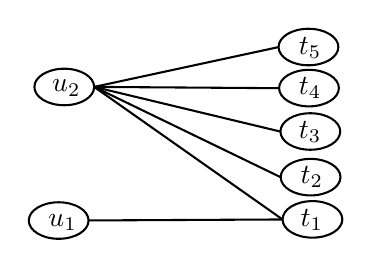
\begin{tikzpicture}[x=0.75pt,y=0.75pt,yscale=-.55,xscale=.9]
%uncomment if require: \path (0,310); %set diagram left start at 0, and has height of 310

%Shape: Circle [id:dp7530951281094582] 
\draw   (257.14,91.73) .. controls (257.17,100.56) and (250.04,107.76) .. (241.2,107.79) .. controls (232.37,107.83) and (225.17,100.7) .. (225.14,91.86) .. controls (225.1,83.02) and (232.23,75.83) .. (241.07,75.79) .. controls (249.91,75.76) and (257.1,82.89) .. (257.14,91.73) -- cycle ;
%Shape: Circle [id:dp9324922852398969] 
\draw   (256.86,55.73) .. controls (256.9,64.56) and (249.76,71.76) .. (240.93,71.79) .. controls (232.09,71.83) and (224.9,64.7) .. (224.86,55.86) .. controls (224.82,47.03) and (231.96,39.83) .. (240.79,39.8) .. controls (249.63,39.76) and (256.82,46.89) .. (256.86,55.73) -- cycle ;
%Shape: Circle [id:dp21183658776860814] 
\draw   (126.14,90.73) .. controls (126.17,99.56) and (119.04,106.76) .. (110.2,106.79) .. controls (101.37,106.83) and (94.17,99.7) .. (94.14,90.86) .. controls (94.1,82.02) and (101.23,74.83) .. (110.07,74.79) .. controls (118.91,74.76) and (126.1,81.89) .. (126.14,90.73) -- cycle ;
%Shape: Circle [id:dp1138329234262836] 
\draw   (257.86,129.73) .. controls (257.9,138.56) and (250.76,145.76) .. (241.93,145.79) .. controls (233.09,145.83) and (225.9,138.7) .. (225.86,129.86) .. controls (225.82,121.03) and (232.96,113.83) .. (241.79,113.8) .. controls (250.63,113.76) and (257.82,120.89) .. (257.86,129.73) -- cycle ;
%Shape: Circle [id:dp5258577677891723] 
\draw   (123.14,207.73) .. controls (123.17,216.56) and (116.04,223.76) .. (107.2,223.79) .. controls (98.37,223.83) and (91.17,216.7) .. (91.14,207.86) .. controls (91.1,199.02) and (98.23,191.83) .. (107.07,191.79) .. controls (115.91,191.76) and (123.1,198.89) .. (123.14,207.73) -- cycle ;
%Shape: Circle [id:dp23423166586948985] 
\draw   (258,169.73) .. controls (258.03,178.56) and (250.9,185.76) .. (242.06,185.79) .. controls (233.23,185.83) and (226.03,178.7) .. (226,169.86) .. controls (225.96,161.03) and (233.09,153.83) .. (241.93,153.79) .. controls (250.76,153.76) and (257.96,160.89) .. (258,169.73) -- cycle ;
%Shape: Circle [id:dp9473655596063126] 
\draw   (259,206.73) .. controls (259.03,215.56) and (251.9,222.76) .. (243.06,222.79) .. controls (234.23,222.83) and (227.03,215.7) .. (227,206.86) .. controls (226.96,198.03) and (234.09,190.83) .. (242.93,190.79) .. controls (251.76,190.76) and (258.96,197.89) .. (259,206.73) -- cycle ;
%Straight Lines [id:da9982536095158081] 
\draw    (123.14,207.73) -- (227,206.86) ;
%Straight Lines [id:da47969048910504686] 
\draw    (126.14,90.73) -- (226,169.86) ;
%Straight Lines [id:da04357275217194001] 
\draw    (126.14,90.73) -- (225.86,129.86) ;
%Straight Lines [id:da5426269746436285] 
\draw    (126.14,90.73) -- (225.14,91.86) ;
%Straight Lines [id:da23827025163526505] 
\draw    (126.14,90.73) -- (224.86,55.86) ;
%Straight Lines [id:da8587083135549514] 
\draw    (126.14,90.73) -- (227,206.86) ;


% Text Node
\draw (234,80) node [anchor=north west][inner sep=0.75pt]   [align=left] {{$t_4$}};
% Text Node
\draw (234,45) node [anchor=north west][inner sep=0.75pt]   [align=left] {{$t_5$}};
% Text Node
\draw (102,82) node [anchor=north west][inner sep=0.75pt]   [align=left] {{$u_2$}};
% Text Node
\draw (100,200) node [anchor=north west][inner sep=0.75pt]   [align=left] {{$u_1$}};
% Text Node
\draw (234,118) node [anchor=north west][inner sep=0.75pt]   [align=left] {{$t_3$}};
% Text Node
\draw (235,158) node [anchor=north west][inner sep=0.75pt]   [align=left] {{$t_2$}};
% Text Node
\draw (235,195) node [anchor=north west][inner sep=0.75pt]   [align=left] {{$t_1$}};
\end{tikzpicture}
\caption{The described instance $\inst$ with $\prob=1/2$ and $\sigmabf = (t_1, \ldots, t_5)$.}\label{fig:instance_generalized_imbalance}
\end{figure}

 First off, observe that  a possible realization of $\greedy$ results in every arrival being matched to $u_2$, so $\greedy(\inst) = 1 - (1/2)^5$.  Next, notice that $\offI(\inst) \geq 3/2$ by matching $t_1$ to $u_1$ and $t_2$ and $t_3$ can be matched fully to $u_2$. Finally, notice that the instance admits a $2$-imbalanced pair $(\undersup, \oversup) = (\{ u_2 \}, \{ u_1\})$ because reducing the capacity of $u_1$ to $1/2$ does not affect the optimal solution whereas increasing the capacity of $u_2$ to $2$ increases the objective by $(\market-1)=1$, as it allows to additionally match $t_4$ and $t_5$ to $u_2$. Combining all these we find that
\begin{equation*}
    \frac{\mathbb E[\greedy(\inst, \sigmabf)]}{\offI(\inst)} \leq \frac{1 - (1/2)^5}{3/2} = \frac{2}{3} \cdot (1 - (1/2)^5) < \frac{2}{3} \leq \frac{\mathbb E[\altgreedy(\inst, \sigmabf, (\undersup, \oversup))]}{\offI(\inst)}.
\end{equation*}
\section{The tradeoff between tighter benchmarks}

% \dfcomment{first, introduce the fact that there are tighter benchmarks}
{Recent work in online bipartite matching has introduced tighter benchmarks that allow for tighter CR guarantees. Notable examples include the Configuration LP proposed by \citet{huang2020online}, the Path-Based Program by \citet{goyal2023online} for adversarial arrivals, and the benchmark introduced by \citet{brubach2020online} for stochastic arrivals.} Despite their ability to provide sharper performance guarantees, tighter benchmarks come with a substantial computational cost. In this section, we illustrate, with a focus on the Path-Based Program by \citet{goyal2023online}, how the exponential complexity inherent in these benchmarks makes them difficult to use in practice, even for small instances.

We begin by defining the set $\Omega$ of \emph{sample paths}, where each $\omega \in \Omega$ indicates which edges in $E$ realize (success of consumption) and which do not. Since each edge may independently succeed or fail, the size of this sample space grows exponentially with $|E|$, in particular, $|\Omega| = 2^{|E|}$. In this section, we focus on the \emph{Path-Based Program} (PBP) as described in \citet{goyal2023online}, a tighter benchmark that exploits this sample space. Although PBP has an exponential number of constraints, it is still possible -- at least in principle -- to simulate it. As we will see, however, this simulation fails to accurately describe the value of PBP even on small instances.

 We now introduce the path-based formulation, whose decision variables  $(\xbf^\omega)_{\omega \in \Omega}$ represent if an offline algorithm (that knows the input graph in advance), matches $u$ to $t$ in the sample path $\omega$.
\begin{align}
\mathrm{PBP}(\inst) = \max_{\mathbf{x}} \quad &  \mathbb E_{\omega} \left[ \sum_{(u,t) \in E} x_{u,t}^\omega  \cdot \bm{1}^\omega_{(u,t) \in E} \right] \label{pbp: obj}\\
\text{s.t.} \quad & \sum_{t: (u,t) \in E} x_{u,t}^\omega  \cdot \bm{1}^\omega_{(u,t) \in E} \leq 1, & \forall u \in \supply, \omega \in \Omega \label{pbp: supply}\\
& \sum_{u: (u,t) \in E} x_{u,t}^\omega  \leq 1, & \forall t \in [T], \omega \in \Omega \label{pbp: demand}\\
& x^\omega_{u,t} = x^{\omega'}_{u,t} &\forall (u,t) \in E, \omega, \omega' \in \Omega: \omega_{-ut} = \omega'_{-ut} \label{pbp: exp}\\
& 0 \leq x^\omega_{u,t} \leq 1, & \forall (u,t) \in E, \omega \in \Omega. \label{pbp: relax}
\end{align}
\noindent
%We next discuss the role of each constraint in the PBP formulation.
Constraint $ (\ref{pbp: supply}) $ enforces that every supply node can be consumed at most once whenever the edge $ (u,t) $ is present in $ E $ and realizes in the sample path $ \omega $.
Similarly, constraint $ (\ref{pbp: demand}) $ ensures that $ t $ is matched to at most one supply node in every sample path.
Of particular interest is constraint $ (\ref{pbp: exp}) $, which captures the idea that an algorithm must commit to (or refrain from) matching $ (u,t) $ without knowing whether that specific edge will ultimately succeed.
Formally, the choice of matching $ (u,t) $ depends only on the realization of \emph{other} edges, and not on the realization of $ (u,t) $ itself.
Lastly, constraint $ (\ref{pbp: relax}) $ allows fractional decision variables. The objective $ (\ref{pbp: obj}) $ takes the weighted average (expectation) of these matchings across all realizations.


Since every algorithm must satisfy constraints $ (\ref{pbp: supply}) $, $ (\ref{pbp: demand}) $, $ (\ref{pbp: exp}) $, and $ (\ref{pbp: relax}) $, the value of $ \pbp $ provides a valid upper bound for any algorithm.
Note the one-to-one correspondence between the supply and demand constraints $ (\ref{pbp: supply}) $, $ (\ref{pbp: demand}) $ of $ \pbp $ and the supply and demand constraints $ (\ref{adversarial_lp: kappa-constraint}) $, $ (\ref{adversarial_lp: demand_constraint}) $ of $ \offI(\inst) $.
Since the constraints of $ \pbp $ hold for every sample path---whereas those of $ \offI(\inst) $ hold only in expectation---the path-based formulation provides a strictly tighter upper bound.

\subsection{The infeasibility of computing PBP for large instances}
\label{ssec: pbp_infeasible}
%\bbcomment{changed small instances to large instances in the title}

The tighter upper bound of PBP comes with a significant disadvantage: to solve the relaxation exactly, one needs to (i) enumerate all sample paths in $\Omega$, and (ii) enumerate,  for each edge $(u,t)$, \emph{all} pairs of sample paths 
whose realizations differ solely in the realization of $(u,t)$. 
Concretely, we have $\vert \Omega \vert = 2^{|E|}$, and the number of subsets of the form
$\{\,(\omega,\omega') \in \Omega^2 : \omega_{-ut} = \omega'_{-ut}\}$
has size $2^{|E|+1}$. 
This holds because each of the $|E|-1$ other edges has two possible outcomes (success/failure), which 
leads to $2^{|E|-1}$ assignments, 
and for each such assignment, $(u,t)$ can be realized or not in both $\omega$ and $\omega'$; thus, there are four distinct ways to define $(\omega,\omega')$ for that fixed assignment. As a result, computing $\pbp$ even for small instances requires significant computational effort and becomes intractable rapidly.

A natural approach to circumvent this complexity is by simulating only a subset of sample paths. Concretely, fix a sample size $n_s$ and draw $n_s$ realizations of $E$ where each edge succeeds w.p. $\prob$. This generates a set of sample paths $\Omega_{n_s} \subseteq \Omega$ and one can then replace $\Omega$ by $\Omega_{n_s}$ in the definition of $\pbp$. However, as we next discuss, this approach may fail to yield an upper bound on the true value of $\pbp$. 
%By sampling finitely many paths, we may omit significant regions of the sample space, 
%including those that could constrain the optimal matching more severely. In what follows, we describe a instance that suppose a problem to simulate PBP.

% \dfcomment{HW for Benjamin: find an instance that is as small as possible; one which you can compute PBP exactly; but which has the property that sampled PBP (at least for 10 and 100 samples; at least for some values of $\prob$ is larger than OFF). Add that instance (as a graph) to the doc; as a new figure; and replace the corresponding figures 7 and 8.} \bbcomment{Replaced with the figure we talked}

%There are two main reasons why sampling-based methods may fail to provide an accurate estimation of $\pbp$. 
The main reason why sampling-based $\pbp$ may yield a worse bound than $ \offI(\inst) $ relates to constraint \eqref{pbp: exp}, which acts as a linking constraint between sample paths. 
In the absence of that constraint, $\pbp$ can solve a maximum matching on the graph of realized edges. For example, if $\prob=1/2$ and a node $t$ has 6 neighbors, then with probability $63/64$ at least one of the incident edges realizes, meaning that on about 63 out of 64 sample paths, $\pbp$ without \eqref{pbp: exp} can successfully match that node in a maximum matching. In contrast, both $\offI(\inst)$ and any adaptive algorithm have a chance of at most $1/2$ to assign that node $t$. Now, \eqref{pbp: exp} ensures that this issue does not occur for $\pbp$, but we argue that for sample-based $\pbp$ to include \emph{any} constraints of the form \eqref{pbp: exp}, the number of samples needs to be exponential in $|E|$. Specifically, this holds true because, for any edge $(u,t)$ and sample path $\omega$, the probability that a different sampled sample path $\omega'$ coincides with $\omega$ on all but one value is $(1/2)^{|E|-1}$ (for $\prob=1/2$). Therefore, unless one samples an exorbitant number of edges, even for medium-sized graphs, the sampled version of $\pbp$ is likely to yield a worse bound than $\offI(\inst)$ would.

% can assign a node, on a given sample path, based on the realization of its incident edges. In other words, $\pbp$ solves
% When the number of samples is small, a given sample path $\omega$ may not have any other sample path $\omega'$ such that $\omega_{-ut} = \omega'_{-ut}$. In such cases, constraint \eqref{pbp: exp} becomes effectively inapplicable for certain $\omega$, leading the optimization problem to produce a perfect matching for these sample paths, thereby artificially inflating the objective function. The second reason, more inherent to Monte Carlo methods, is the difficulty in accurately approximating the probability of a sample path occurring due to the exponential nature of the optimization problem. However, as shown in \Cref{fig: pbpbad1hist}, increasing the number of samples is not a feasible solution to these issues for large instances, as doubling the sample since leads to at least a 400\% increase in computation time. \dfcomment{is the second issue really insightful? I think the first one is the key point! if i understand you right, you are saying: without (23), each demand node can be matched based after the edges realize (rather than before); but if we sample just $poly(|E|)$ edges, and $|E|$ grows large, we should not expect to catch any of the (23) constraints (especially when $\prob$ is close to 1 and the variance of outcomes is largest). is that right?}

We now numerically illustrate this finding about sampled-PBP. We rely on the graph structure in \Cref{fig:instance_pbp} and vary $\prob$ at 40 equidistant values from $10^{-2}$ to $1$; for each $\prob$, we simulate $\pbp$, with either 100, 500, or 1000 sample paths, 30 times and average the result. 
\Cref{fig: pbpbad1} illustrates the poor convergence of these sampled versions of $\pbp$. Though $ \pbp $ is a tighter benchmark than $ \offI(\inst) $, and thus lies below it, the curves corresponding to the sampling approach often lie above $ \offI(\inst) $, even for $n_s=1000$ and in an instance with just 8 edges. %However, even in this small instance with just eight edges, we observe that sampling-based methods also face convergence difficulties. 
\Cref{fig: pbpbad1hist} also shows that the computational effort of this sampling approach rapidly increases with $n_s$. As a result, we view these state-of-the-art benchmarks as mostly useful for the theoretical design of algorithms, but not to numerically evaluate algorithms. 
% or defining concepts like imbalance.\dfcomment{is that the right point here?}
% an instance with two types of supply nodes and two types of demand arrivals. Within each supply type there is only one single node, and within each demand type there are two nodes. The edges between demand nodes and supply nodes follow the next pattern: demand nodes of type 1 are connected to the two supply nodes; demand nodes of type 2 are only connected to supply nodes of type 2. The two demand arrivals of type 1 arrive first, followed by the two demand arrivals of type 2.
% ; demand nodes of type 3 are connected to all supply nodes except those of supply types 1 and 2; and demand nodes of type 4 are connected only to the supply nodes of type 4.
% We set $\prob$ taking 20 equidistant values from $10^{-2}$ to $1$, and for each $\prob$, we sample $\pbp$ 30 times and average the result.

%\dfcomment{add the graph as figure 7 to the left of the other two; all three should fit next to each other (increase the font size of labels etc) to increase the } \bbcomment{done}
\begin{figure}[h]
    \centering
        \begin{minipage}{0.29
        \textwidth}
        \centering
        \includegraphics[width=\textwidth]{images/bad_instance_2.pdf}
        \caption{\small{Graph structure considered for the tests.}}
        \label{fig:instance_pbp}
    \end{minipage}\hfill
    \begin{minipage}{0.33\textwidth}
        \centering
        \includegraphics[width=\textwidth]{images/pbpbadinstance1_2.pdf}
        \caption{\small{Comparison of sampling PBP (number of samples).}}
        \label{fig: pbpbad1}
    \end{minipage}\hfill
    \begin{minipage}{0.33\textwidth}
        \centering
        \includegraphics[width=\textwidth]{images/pbpbadinstance1hist_2.pdf}
        \caption{\small{Histogram representing the total time taken for each sampled PBP method.}}
        \label{fig: pbpbad1hist}
        \vfill \hfill
    \end{minipage}
    %\vspace{-.15in}
\end{figure}








%The primary reason for this behavior lies in how sampling handles the constraints of $ \pbp $. For any $\prob$, there is a significant chance that $ \Omega_{n_s} $ (the sampled set of scenarios) fails to capture the entirety of $ \Omega $. As a result, the sampled method may not necessarily produce a tighter bound than $ \offI(\inst) $, since some constraints are effectively missing. Another issue arises when sample paths with low probability appear too infrequently, meaning they do not adequately influence the objective value. Nonetheless, as seen in \Cref{fig: pbpbad1hist}, simply increasing the number of samples is impractical for large instances: moving from 100 to 500 samples alone can lead to a computational increase of over 500 seconds.\dfcomment{the absolute increase is irrelevant (always report relative in such a case); and also, it is not clear that we are talking about large instances here. }

\subsection{Numerical Evaluation of instantaneous algorithms under Imbalanced Instances}

\label{ssec:imbalanced}

The main goal of this subsection is to illustrate that in highly imbalanced settings, both delayed and instantaneous algorithms produce better CRs. 
In \Cref{section: impossibility}, we introduced a class of instances $\inst_s[\market]$, parameterized by $s$ and $\market$, to prove the tightness result of \Cref{prop: adversarial CR UB}. Here, we focus on a simplified version of those instances and numerically compare the performance of $\greedy$ and the generalized fully-adaptive algorithm of \citet{goyal2023online}.

We set $L = 10$ and $\prob = 1/100$. We use an upper triangular instance as our test instance; it consists of 10 demand types and 10 supply nodes, structured so that demand nodes of type 1 connect to every supply type 1, demand nodes of type 2 connect to all supply nodes except for node 1, demand nodes of type 3 connect to all except for nodes 1 and 2, and so forth. Each type of demand consists of $\lceil \market / \prob \rceil$ nodes (with demand type 1 arriving first, then 2, and so forth), where $\market$ takes 40 logarithmically spaced values between $10^{-1.2}$ and $10^{1.2}$. For each instance considered, we compute $\greedy(\inst)$, $\offI(\inst)$, and the generalized fully-adaptive algorithm a total of {1,500} times, taking their mean. We plot the results in \Cref{fig: goyal_greedy_comparison}.
\begin{figure}[h]
    \centering
    \includegraphics[width=0.5\linewidth]{images/goyal_greedy_comparison_with_CI_2.pdf}
    \caption{Comparative analysis of CRs between $\greedy$  and the generalized fully-adaptive algorithm from \citet{goyal2023online} across the described class of instances. Each data point represents the mean CR obtained from 1,500 simulation runs; the shaded regions denote {95\% confidence intervals}. }
    \label{fig: goyal_greedy_comparison}
\end{figure}


As \Cref{fig: goyal_greedy_comparison} shows, unsurprisingly and in line with \Cref{prop: adversarial CR UB}, the CR of $\greedy$ is close to its theoretical lower bound. We also observe the difference of instantaneous feedback in these instances: the generalized fully-adaptive algorithm consistently obtains better CRs than $\greedy$ for all of the considered instances. As the imbalance $\market$ becomes large or small, both algorithms approach a CR of 1 at a similar rate, indicating that imbalance yields better CR guarantees for instantaneous algorithms also, not just for $\greedy$ which our theoretical analysis revealed. 

{Lastly, we remark that the wider confidence intervals for small $\market$ arise from the scale of $\offI(\inst)$ (proportional to $\market L$) and the structure of the instance. For lower values of $\market$, the variance increases since there are fewer demand nodes per type, which makes it more likely for algorithms to assign demand nodes to supply nodes that will no longer be available for future demand arrivals.}





% Consequently, reducing the variance sufficiently to shrink the confidence intervals would require a significantly larger number of samples.





\subsection{Computation of $\market$ on a given instance}
\label{ssec: computation_kappa_instance}

Given $\xbf^*$ an optimal solution to \ref{prob: convex}, we compute the imbalance of an imbalanced pair $(\undersup, \oversup)$ via the following optimization problem:
\begin{align}
\max_{\market,\, z,\, \mathbf{x}} \quad 
& \market  \notag\\
\text{s.t.}\quad 
& \market \cdot z \;=\; 1, \label{cons: kappa_z}\\
& \sum_{t : (u,t) \in E} \prob \cdot x_{u,t} \leq \market,
  \quad \forall\, u \in \undersup, \label{cons: kappa_undersup}\\
& \sum_{t : (u,t) \in E} \prob \cdot x_{u,t} \leq z,
  \quad \forall\, u \in \oversup, \label{cons: kappa_oversup}\\
& \sum_{u : (u,t) \in E} x_{u,t} \leq 1,
  \quad \forall\, t \in [T], \label{cons: kappa_demand}\\
& \sum_{(u,t) \in E: u \in \undersup}
    \prob \cdot x_{u,t} 
  = \market  |\undersup|, \label{cons: kappa_undersup_guarantee}\\
& \sum_{(u,t) \in E: u \in \oversup}
    \prob \cdot x_{u,t} =
  \sum_{(u,t) \in E : u \in \oversup}
      \prob \cdot x^*_{u,t}, \label{cons: kappa_oversup_guarantee}\\
& \mathbf{x} \;\ge\; \mathbf{0}, 
  \quad \market \;\ge\; 1, 
  \quad z \;\ge\; 0 \label{cons: kappa_feasibility}.
\end{align}

As observed, this optimization problem is \textit{non-convex}, primarily due to constraint \eqref{cons: kappa_z}. This constraint, together with \eqref{cons: kappa_oversup}, enforces that $\sum_{t : (u,t) \in E} \prob \cdot x_{u,t} \leq 1/\market, \forall u \in \oversup$, ensuring that condition (iii) of \Cref{def: new_over_undersupplied} holds. Given that solving non-convex problems is NP-hard and may require exponential time, it is practical to consider an alternative approach for computing $\market$. Specifically, by first computing $\offI(\inst)$ and with knowledge of $\undersup$ and $\oversup$, one can employ a binary search on $\market$ in the right-hand side constraint of \ref{prob: offlineUndersupplied}. In this process, conditions (ii) and (iii) in \Cref{def: new_over_undersupplied} are ensured at each step. While the binary search itself is logarithmic in the range size, the complexity of each step depends on solving a LP, resulting in an overall polynomial time complexity.

We now state and show that the previous non-convex problem objective is $\market$, for some $\market$-imbalance pair.


\noindent\textit{Claim.}
    Given $(\undersup, \oversup)$ a $\market$-imbalance pair and $x^*$ an optimal solution to \ref{prob: convex}, then the above optimization problem returns $\market$.

\noindent \textbf{Proof of Claim.} Start off by noting that the set of constraints is feasible: the solution $(\market, z, \xbf) = (1,1,\xbf^*)$ satisfies all the constraints. Since $\xbf^*$ is an optimal solution to $\offI(\inst)$, then the set of constraints \eqref{cons: kappa_undersup}, \eqref{cons: kappa_oversup} are exactly the set of constraints \eqref{adversarial_lp: kappa-constraint} with $\market = 1$. Constraint \eqref{cons: kappa_demand} is exactly constraint \eqref{adversarial_lp: demand_constraint}. Constraint \eqref{cons: kappa_undersup_guarantee} follows by definition of $\classU = \undersup$, the set of consumed nodes by $\xbf^*$ (where the equality follows by \Cref{prop: k-imbalanced result}). The rest of the constraints follows directly.

Now, let $(\market, z, \xbf)$ an optimal solution to the above problem. We show that $\xbf$ is optimal for \ref{prob: offlineUndersupplied}:
\begin{align*}
    \sum_{(u,t) \in E : u \in \undersup} \prob \cdot x_{u,t} + \sum_{(u,t) \in E : u \in \oversup} \prob \cdot x_{u,t} &= \market \cdot |\undersup|  + \sum_{(u,t) \in E : u \in \oversup} \prob \cdot x_{u,t}\\
    &= \market \cdot |\undersup|  + \sum_{(u,t) \in E : u \in \oversup} \prob \cdot x^*_{u,t}\\
    &= (\market -1)  |\undersup| + \offI(\inst).
\end{align*}
The first equality uses constraint \eqref{cons: kappa_undersup_guarantee}. The second equality uses constraint \eqref{cons: kappa_oversup_guarantee} and the last equality uses $\sum_{(u,t) \in E : u \in \undersup} \prob \cdot x^*_{u,t} = |\undersup|$ and that $x^*$ is optimal for $\offI(\inst)$.
Since constraints \eqref{cons: kappa_undersup}, \eqref{cons: kappa_oversup}, \eqref{cons: kappa_demand} and \eqref{cons: kappa_feasibility} impose feasibility of $\xbf$, we have that $\xbf$ is an optimal solution to \ref{prob: offlineUndersupplied}.
Finally, the objective  ensures that we find the maximum $\market$ for which constraints \eqref{cons: kappa_undersup}, \eqref{cons: kappa_oversup} ensure that $\xbf$ is optimal in \ref{prob: offlineUndersupplied}. %, respectively over-, supplied.to finding the maximum $\market$ that satisfies that . 